% Copyright 2026 Sreeram Anil
% SPDX-License-Identifier: CC-BY-4.0
% =============================================================================
%  Adaptive Kalman family — chapter order
%
%  The order is pedagogical: first the three filters that estimate the
%  measurement-noise covariance R from the innovation sequence (recursive MAP,
%  windowed covariance matching, variational Bayes), then the fuzzy supervisor
%  that is a rate-limited version of the same idea, then the two filters that
%  inflate the state covariance P instead (strong tracking, fading memory), and
%  finally the two multiple-model estimators that carry the competing
%  hypotheses explicitly (IMM over noise regimes, MMAE over model parameters).
%  Later chapters reference equations and assumptions introduced in earlier
%  ones, so this order should be preserved.
% =============================================================================

% Copyright 2026 Sreeram Anil
% SPDX-License-Identifier: CC-BY-4.0
% =============================================================================
%  Sage--Husa adaptive extended Kalman filter
% =============================================================================
\chapter{Sage--Husa adaptive extended Kalman filter (SageHusa-AKF)}
\label{ch:sagehusaakf}

\section*{At a glance}
\begin{tabular}{@{}l>{\raggedright\arraybackslash}p{0.76\textwidth}@{}}
Family & Adaptive Kalman \\
Header & \texttt{include/estkit/filters/sage\_husa\_akf.hpp} \\
Registered name & \texttt{SageHusa-AKF} \\
State dimension & $n_x = 4$ (cell model) --- generic in $n_x, n_u, n_y$ \\
Cost per step & $\mathcal{O}(n_x^3)$, EKF $+\,\mathcal{O}(n_y^2 n_x)$; $\approx 545$\,ns/step measured, no heap \\
Primary references & \cite{sagehusa1969,sagemelsa1971,maybeck1979,jazwinski1970} \\
\end{tabular}

\section{Motivation and aerospace/BMS relevance}
The Kalman filter is optimal only when the noise covariances $\mQ$ and $\mR$ that it is given are
the ones that actually generated the data.  In a battery-management system neither is known.  The
measurement-noise covariance $\mR$ is dominated by the voltage front end, whose effective noise
changes with temperature, with the switching state of the power stage, and --- in a flight vehicle
--- with the electromagnetic environment: an inverter commutating at high power can raise the
apparent voltage noise of a cell-sense channel by an order of magnitude within one flight phase.
A filter tuned for the quiet ground-test value of $\sigma_v$ then trusts a noisy measurement far
too much: its innovations become inconsistent with its own covariance, the state estimates chase
sensor noise, and any innovation-based fault monitor downstream (a standard element of a DO-178/
DO-254 class health-management chain, cf.\ the environmental qualification philosophy of
\cite{rtca2017do311a}) raises spurious alarms.

Sage and Husa \cite{sagehusa1969} were the first to give a \emph{recursive} answer: treat the
unknown noise statistics as parameters, write down the maximum-a-posteriori (MAP) estimate of those
parameters given the data seen so far, and evaluate it with an exponentially weighted (forgetting)
average so that the resulting estimator can track slow changes.  The method is attractive for
embedded use precisely because the result is a one-line recursion that re-uses quantities the
Kalman filter already computes --- the innovation, the residual and the updated covariance --- and
adds no matrix inversion and no storage beyond one $n_y\times n_y$ matrix.

The price is that the same derivation applied to the process-noise covariance $\mQ$ produces a
recursion whose increment is a \emph{difference} of covariances, and which therefore loses positive
definiteness in practice.  This chapter implements the $\mR$ recursion in its positive-definite
(residual) form as the default, keeps the $\mQ$ recursion available but disabled, and explains why.

\section{Problem statement and assumptions}
The plant is the usual discrete-time nonlinear model of \cref{ch:ecm},
\begin{align}
\vx_{k} &= f(\vx_{k-1}, \vu_{k-1}) + \vw_{k-1}, & \vw_k &\sim \N{\bm{0}}{\mQ_k}, \label{eq:sh:proc}\\
\vy_{k} &= h(\vx_{k}, \vu_{k}) + \vv_{k},       & \vv_k &\sim \N{\bm{0}}{\mR_k}, \label{eq:sh:meas}
\end{align}
where $\vx_k\in\real^{n_x}$ is the state, $\vu_k\in\real^{n_u}$ the (known) input, $\vy_k\in\real^{n_y}$
the measurement, and $\vw_k, \vv_k$ are mutually independent zero-mean white sequences.  The
functions $f$ and $h$ are known; $\mR_k$ is \emph{not}.  We assume

\begin{assumption}\label{as:sh:slow}
$\mR_k$ is constant over a window of length $\tau_R = 1/(1-b)$ samples, $b\in(0,1)$, but may change
between such windows.  Equivalently, $\mR$ is a slowly varying deterministic sequence compared with
the filter's own time constants.
\end{assumption}
\begin{assumption}\label{as:sh:lin}
The linearisation $\mH_k = \partial h/\partial\vx|_{\xminus_k}$ is accurate over the region spanned by
$\Pminus_k$, so that the innovation covariance predicted by the filter is
$\mS_k=\mH_k\Pminus_k\mH_k^\T+\mR_k$.
\end{assumption}

The quantity to be estimated jointly with $\vx_k$ is $\mR_k\in\real^{n_y\times n_y}$, symmetric
positive definite.

\section{Derivation}

\subsection{MAP estimate of the noise statistics}
Sage and Husa \cite{sagehusa1969} (see also \cite[Ch.~9]{sagemelsa1971}) consider the joint
posterior of the state trajectory and the unknown noise statistics and maximise it with respect to
the statistics while holding the trajectory at its filtered estimate.  With $\mR$ constant over
$k=1,\dots,N$ and a flat prior, the log-posterior contributed by the measurements is
\begin{equation}
\mathcal{L}(\mR) = -\tfrac{1}{2}\sum_{j=1}^{N}\Big[\,\ln\det\mR + (\vy_j-h(\vx_j,\vu_j))^\T \mR\inv (\vy_j-h(\vx_j,\vu_j))\,\Big] + \text{const}.
\label{eq:sh:loglik}
\end{equation}
Setting $\partial\mathcal{L}/\partial \mR\inv = \bm{0}$ gives the familiar sample-covariance form
\begin{equation}
\hat{\mR} = \frac{1}{N}\sum_{j=1}^{N} \E{(\vy_j-h(\vx_j,\vu_j))(\vy_j-h(\vx_j,\vu_j))^\T \mid \vy_{1:N}}.
\label{eq:sh:Rmap}
\end{equation}
The conditional expectation in \eqref{eq:sh:Rmap} cannot be evaluated exactly, because $\vx_j$ is
unknown; replacing it by the filtered estimate $\xplus_j$ and accounting for the remaining
uncertainty $\Pplus_j$ to first order in the linearisation of \cref{as:sh:lin} gives, with the
\emph{a-posteriori residual}
\begin{equation}
\bm{r}_j \triangleq \vy_j - h(\xplus_j,\vu_j) \in\real^{n_y},
\label{eq:sh:resid}
\end{equation}
the estimator
\begin{equation}
\boxed{\;\hat{\mR} = \frac{1}{N}\sum_{j=1}^{N}\Big[\bm{r}_j\bm{r}_j^\T + \mH_j\Pplus_j\mH_j^\T\Big].}
\label{eq:sh:Rresid}
\end{equation}
The second term corrects for the fact that the residual $\bm{r}_j$ is \emph{smaller} than the true
measurement noise: part of the noise has already been absorbed into $\xplus_j$.  Explicitly, from
$\bm{r}_j=\vv_j-\mH_j(\xplus_j-\vx_j)+\mathcal{O}(\|\cdot\|^2)$ and
$\E{(\xplus_j-\vx_j)\vv_j^\T} = -\mK_j\mR_j$ one obtains
$\E{\bm{r}_j\bm{r}_j^\T} = \mR_j - \mH_j\Pplus_j\mH_j^\T$, which is exactly what \eqref{eq:sh:Rresid}
inverts.  Both terms on the right of \eqref{eq:sh:Rresid} are positive semi-definite; this is the
key structural property exploited below.

An algebraically equivalent expression follows by using the \emph{a-priori} innovation
$\bm{e}_j=\vy_j-h(\xminus_j,\vu_j)$, for which $\E{\bm{e}_j\bm{e}_j^\T}=\mH_j\Pminus_j\mH_j^\T+\mR_j$:
\begin{equation}
\hat{\mR} = \frac{1}{N}\sum_{j=1}^{N}\Big[\bm{e}_j\bm{e}_j^\T - \mH_j\Pminus_j\mH_j^\T\Big].
\label{eq:sh:Rinnov}
\end{equation}
Equation~\eqref{eq:sh:Rinnov} is the innovation form; it is unbiased but, being a difference of two
positive semi-definite matrices, it is \emph{not} guaranteed to be positive definite for finite $N$.

\subsection{Recursive evaluation with a forgetting factor}
Neither \eqref{eq:sh:Rresid} nor \eqref{eq:sh:Rinnov} can be evaluated as written on an embedded
target: they need the whole history.  Writing the sample mean recursively,
$\hat{\mR}_k = \hat{\mR}_{k-1} + \tfrac{1}{k+1}(\text{increment}_k - \hat{\mR}_{k-1})$, and replacing
the uniform weight $1/(k+1)$ by the normalised exponential weight of a forgetting factor
$b\in(0,1)$ gives the Sage--Husa weight sequence
\begin{equation}
d_k = \frac{1-b}{1-b^{\,k+1}}, \qquad d_0 = 1, \qquad \lim_{k\to\infty} d_k = 1-b .
\label{eq:sh:dk}
\end{equation}
$d_k$ is exactly the weight that makes $\hat{\mR}_k$ the \emph{normalised} exponentially weighted
average $\hat{\mR}_k = \sum_{j=0}^{k} b^{\,k-j}\,\text{incr}_j \big/ \sum_{j=0}^{k} b^{\,k-j}$, so the
estimator is unbiased from the first sample on and degenerates smoothly into a sliding exponential
window of effective length $\tau_R = 1/(1-b)$ samples.  The recursion is
\begin{equation}
\hat{\mR}_k = (1-d_k)\,\hat{\mR}_{k-1} + d_k\Big[\bm{r}_k\bm{r}_k^\T + \mH_k\Pplus_k\mH_k^\T\Big].
\label{eq:sh:Rrec}
\end{equation}

\begin{proposition}[Positive definiteness]\label{prop:sh:pd}
If $\hat{\mR}_{-1}\succ 0$ and $d_k\in[0,1]$ for all $k$, then $\hat{\mR}_k\succ 0$ for all $k$.
\end{proposition}
\begin{proof}
$\bm{r}_k\bm{r}_k^\T\succeq 0$ and $\mH_k\Pplus_k\mH_k^\T\succeq 0$ because $\Pplus_k\succeq 0$.  A convex
combination of a positive definite matrix and a positive semi-definite one with weights
$(1-d_k, d_k)$, $d_k<1$, is positive definite; for $d_k=1$ (only $k=0$) the result is positive
definite provided $\bm{r}_0\neq\bm 0$, and the implementation's diagonal floor
(\cref{sec:sh:impl}) covers the degenerate case.
\end{proof}
The corresponding recursion built on \eqref{eq:sh:Rinnov} carries no such guarantee, which is the
practical reason for preferring \eqref{eq:sh:Rrec}.  Both are implemented
(\texttt{opts.residual\_form}); the innovation form is additionally projected onto the positive
definite cone by the diagonal floor.

\subsection{Why the process-noise recursion is disabled}
Applying the same MAP argument to $\mQ$ yields \cite{sagehusa1969}
\begin{equation}
\hat{\mQ}_k = (1-d_k)\hat{\mQ}_{k-1} + d_k\Big[\mK_k\bm{e}_k\bm{e}_k^\T\mK_k^\T + \Pplus_k - \mF_{k-1}\Pplus_{k-1}\mF_{k-1}^\T\Big].
\label{eq:sh:Qrec}
\end{equation}
The bracket is a \emph{difference}: $\Pplus_k-\mF\Pplus_{k-1}\mF^\T$ is the change of the filtered
covariance over one step, which for a converged filter is a small quantity of either sign, obtained
by cancellation of two nearly equal $\mathcal{O}(\|\mP\|)$ terms.  Three consequences follow.  (i)
$\hat{\mQ}_k$ frequently leaves the positive semi-definite cone and must be projected back, which
biases it.  (ii) Simultaneous adaptation of $\mQ$ and $\mR$ is not identifiable from a single
output sequence: only the ratio enters the steady-state gain, so the pair $(\hat{\mQ},\hat{\mR})$
drifts along the manifold of constant gain \cite{mehra1970}.  (iii) In the battery model the
process noise is \emph{structured} --- $\mQ = \bm{b}\bm{b}^\T\sigma_i^2 + \diag(\bm{q}_{\text{floor}})$
with $\bm b = \partial f/\partial i$ --- so an unstructured $\hat{\mQ}$ destroys information that is
genuinely known.  The default is therefore \texttt{adapt\_Q = false}; the option exists so that the
failure mode can be reproduced.

\section{Algorithm}
\begin{algorithm}[H]
\caption{SageHusa-AKF --- one sampling period}
\begin{algorithmic}[1]
\Require $\xplus_{k-1},\Pplus_{k-1},\vu_{k-1},\vy_k,\vu_k,\hat{\mR}_{k-1},d_k$ from \eqref{eq:sh:dk}
\State \textbf{Time update:} $\mF\gets\partial f/\partial\vx|_{\xplus_{k-1}}$;\quad
       $\xminus_k\gets f(\xplus_{k-1},\vu_{k-1})$;\quad
       $\Pminus_k\gets \mF\Pplus_{k-1}\mF^\T+\mQ_k$
\State \textbf{Innovation:} $\mH\gets\partial h/\partial\vx|_{\xminus_k}$;\quad
       $\bm{e}_k\gets\vy_k-h(\xminus_k,\vu_k)$
\State \textbf{Gain:} $\mS_k\gets \mH\Pminus_k\mH^\T+\hat{\mR}_{k-1}$;\quad
       $\mK_k\gets\Pminus_k\mH^\T\mS_k\inv$ \Comment{skip the update if $\mK_k$ is not finite}
\State \textbf{State update:} $\xplus_k\gets\xminus_k+\mK_k\bm{e}_k$
\State \textbf{Covariance (Joseph):} $\Pplus_k\gets(\mI-\mK_k\mH)\Pminus_k(\mI-\mK_k\mH)^\T+\mK_k\hat{\mR}_{k-1}\mK_k^\T$
\State \textbf{Residual:} $\bm{r}_k\gets\vy_k-h(\xplus_k,\vu_k)$
\State \textbf{Noise adaptation} (if $k\ge k_{\text{warm}}$):
       $\hat{\mR}_k\gets(1-d_k)\hat{\mR}_{k-1}+d_k\big[\bm{r}_k\bm{r}_k^\T+\mH\Pplus_k\mH^\T\big]$
\State \textbf{Safeguard:} $\hat{R}_{k,ii}\gets\mathrm{clamp}\big(\hat{R}_{k,ii},\,\rho_{\min}R_{ii},\,\rho_{\max}R_{ii}\big)$, row/column rescaled by $\sqrt{\cdot}$
\State \textbf{Constrain:} $\xplus_k\gets\mathrm{constrain}(\xplus_k)$
\Ensure $\xplus_k,\Pplus_k,\hat{\mR}_k$
\end{algorithmic}
\end{algorithm}
Here $R_{ii}$ denotes the \emph{nominal} model value $\mR(\xminus_k,\vu_k)$ and
$\rho_{\min},\rho_{\max}$ are the option fields \texttt{r\_min\_scale}, \texttt{r\_max\_scale}.

\section{Application to the battery model}
For the 2-RC equivalent-circuit model of \cref{ch:ecm}, $\vx=[\soc,v_1,v_2,h]^\T$, $\vu=[i,T]^\T$
and $y=v$ is a scalar, so $n_y=1$ and $\hat{\mR}_k$ collapses to a single number
$\hat{\sigma}_v^2 + \hat{\sigma}_{R_0 i}^2$ --- the filter estimates the \emph{total} effective
voltage-channel variance, which correctly lumps the sensor noise, the current-sensor noise that
enters through the $R_0 i$ feed-through, and any un-modelled voltage error.  The analytic Jacobian
$\mH = [\,\partial\ocv/\partial \soc,\;-1,\;-1,\;M\,]$ is supplied by \texttt{EcmModel}, so no
numerical differentiation is needed and the extra cost over the EKF is one extra evaluation of $h$
(for $\bm{r}_k$), one $\mH\Pplus\mH^\T$ product and $n_y^2$ scalar operations.

Tuning used in the benchmark: $b = 0.995$, i.e.\ $\tau_R = 200$ samples $=\SI{20}{\second}$ at the
\SI{10}{\hertz} sample rate.  The choice is a compromise between the statistical accuracy of the
variance estimate (the relative standard deviation of a $\chi^2$-type variance estimate over
$\tau_R$ effective samples is $\sqrt{2/\tau_R}=\SI{10}{\percent}$) and the speed with which a real
change of the noise level must be detected (a BMS fault monitor is normally required to react
within seconds, not minutes).  Literature values for $b$ lie in $0.95$--$0.999$; $0.98$ and $0.999$
were also evaluated and change the steady-state metrics by less than $15\,\%$.
$k_{\text{warm}} = 20$ samples of warm-up keep $\hat{\mR}$ at the model value while the filter
recovers from the initial transient, so that the very first (large) residuals, which reflect the
initial state error and not the sensor, do not enter the average.  The safeguards
$\rho_{\min}=0.05$, $\rho_{\max}=5\times 10^3$ bound $\hat\sigma_v$ to
$[0.47,\,148]\,\si{\milli\volt}$ around the nominal \SI{2.1}{\milli\volt}.

\section{Implementation notes}
\label{sec:sh:impl}
\begin{itemize}[leftmargin=1.4em]
\item \textbf{Weight recursion.}  $b^{\,k+1}$ is propagated incrementally
      ($b^{k+1}\!\leftarrow\! b^{k}\cdot b$, one multiply per sample) rather than recomputed; a naive
      implementation that recomputes the power costs $\mathcal{O}(k)$ per step and was measured at
      $3.2\,\si{\micro\second}$/step before the fix versus $0.55\,\si{\micro\second}$/step after.
\item \textbf{Positive definiteness.}  \cref{prop:sh:pd} makes the residual form structurally safe;
      the diagonal clamp is a second line of defence and also caps the adaptation range.  When a
      diagonal entry is clamped, the whole row and column are multiplied by $\sqrt{\hat R^{\text{new}}_{ii}/\hat R^{\text{old}}_{ii}}$
      so that the correlation coefficients, and hence positive semi-definiteness, are preserved.
\item \textbf{Numerical hygiene.}  The Joseph form is used for $\Pplus$, $\mP$ is symmetrised after
      every update, and a non-finite gain causes the update to be skipped (the previous estimate is
      retained) rather than producing NaNs.
\item \textbf{Memory and flops.}  \texttt{sizeof(SageHusaAkf<EcmModel>)} is dominated by the model
      copy; the filter's own state is $n_x+n_x^2+2n_y^2+n_xn_y+n_x^2 = 45$ reals for the cell model.
      Measured cost $\approx\SI{545}{\nano\second}$/step versus \SI{478}{\nano\second}/step for the
      EKF on the benchmark machine, i.e.\ a difference inside the run-to-run scatter.  On a \SI{400}{\mega\hertz}
      Cortex-M7 with single-precision hardware floating point this scales to roughly
      \SI{7}{\micro\second}/step, negligible at \SI{10}{\hertz}.
\item \textbf{float32.}  The recursion involves no subtraction of nearly equal quantities in the
      default (residual) form, so it is well conditioned in single precision; the
      \texttt{-DESTKIT\_FLOAT=ON} build compiles and runs without divergence.
\item \textbf{Limitations.}  The method assumes that everything that inflates the residuals is
      measurement noise.  On scenarios where the innovations are inflated by a \emph{model} error
      (e.g.\ a grown series resistance) the filter dutifully reports a large $\hat\sigma_v$ and
      de-weights the voltage --- helpful for the SOC estimate, but the reported $\hat{\mR}$ must not
      then be interpreted as a sensor diagnostic.
\end{itemize}

\section{Benchmark results}
% Copyright 2026 Sreeram Anil
% SPDX-License-Identifier: CC-BY-4.0
\begin{table}[H]\centering\footnotesize\setlength{\tabcolsep}{4pt}
\caption{SageHusa-AKF: cell-level benchmark on the eVTOL mission (mean over seeds; RMSE and max error in \% SOC; $t_\mathrm{conv}$: first time the error stays below 2\,\% for 60\,s, -- = never; EKF reference: steady-state RMSE of the plain EKF on the same data).}\label{tab:cell_SageHusaAKF}
\begin{tabular}{llrrrrrcrr}\toprule
plant & scenario & RMSE & RMSE$_\mathrm{ss}$ & max & $t_\mathrm{conv}$ [s] & RMSE$_v$ [mV] & div. & EKF ref. & ns/step \\ \midrule
ECM & nominal & 0.24 & 0.04 & 1.08 & 0 & 0.79 & no & 0.05 & 545 \\
ECM & init\_error & 0.13 & 0.07 & 0.63 & 0 & 2.12 & no & 0.05 & 545 \\
ECM & current\_bias & 0.53 & 0.62 & 1.42 & 0 & 0.87 & no & 0.61 & 546 \\
ECM & noise\_step & 0.24 & 0.04 & 1.08 & 0 & 1.01 & no & 0.12 & 543 \\
ECM & outliers & 0.22 & 0.06 & 2.35 & 0 & 1.11 & no & 0.21 & 545 \\
ECM & cold & 0.21 & 0.22 & 1.17 & 0 & 1.89 & no & 0.16 & 543 \\
ECM & hot & 0.15 & 0.04 & 1.00 & 0 & 0.54 & no & 0.03 & 543 \\
ECM & aged\_cell & 1.07 & 1.30 & 2.58 & 0 & 21.77 & no & 1.52 & 546 \\
ECM & param\_mismatch & 0.59 & 0.76 & 1.50 & 0 & 6.12 & no & 1.36 & 544 \\
ECM & sensor\_dropout & 0.23 & 0.08 & 1.08 & 0 & 1.19 & no & 0.46 & 546 \\
ECM & preisach & 0.67 & 0.20 & 1.94 & 0 & 0.82 & no & 0.20 & 547 \\
ECM & combined & 4.95 & 1.98 & 11.81 & 1446 & 13.91 & no & 12.44 & 544 \\
\midrule
SPM & nominal & 3.26 & 3.33 & 3.94 & 0 & 1.16 & no & 3.73 & 510 \\
SPM & init\_error & 3.85 & 3.87 & 4.73 & 9 & 2.24 & no & 3.81 & 507 \\
SPM & current\_bias & 4.86 & 5.57 & 6.22 & 0 & 1.32 & no & 5.69 & 507 \\
SPM & noise\_step & 3.26 & 3.34 & 3.94 & 0 & 2.16 & no & 3.30 & 509 \\
SPM & outliers & 3.24 & 3.19 & 4.54 & 0 & 2.24 & no & 1.99 & 509 \\
SPM & cold & 2.88 & 2.65 & 4.10 & 0 & 15.62 & no & 7.35 & 493 \\
SPM & hot & 1.99 & 2.07 & 2.32 & 0 & 0.71 & no & 2.16 & 512 \\
SPM & param\_mismatch & 0.98 & 1.13 & 1.62 & 0 & 3.50 & no & 3.13 & 505 \\
SPM & sensor\_dropout & 3.49 & 3.57 & 4.20 & 0 & 2.14 & no & 5.31 & 508 \\
\bottomrule\end{tabular}\end{table}

\begin{figure}[H]\centering
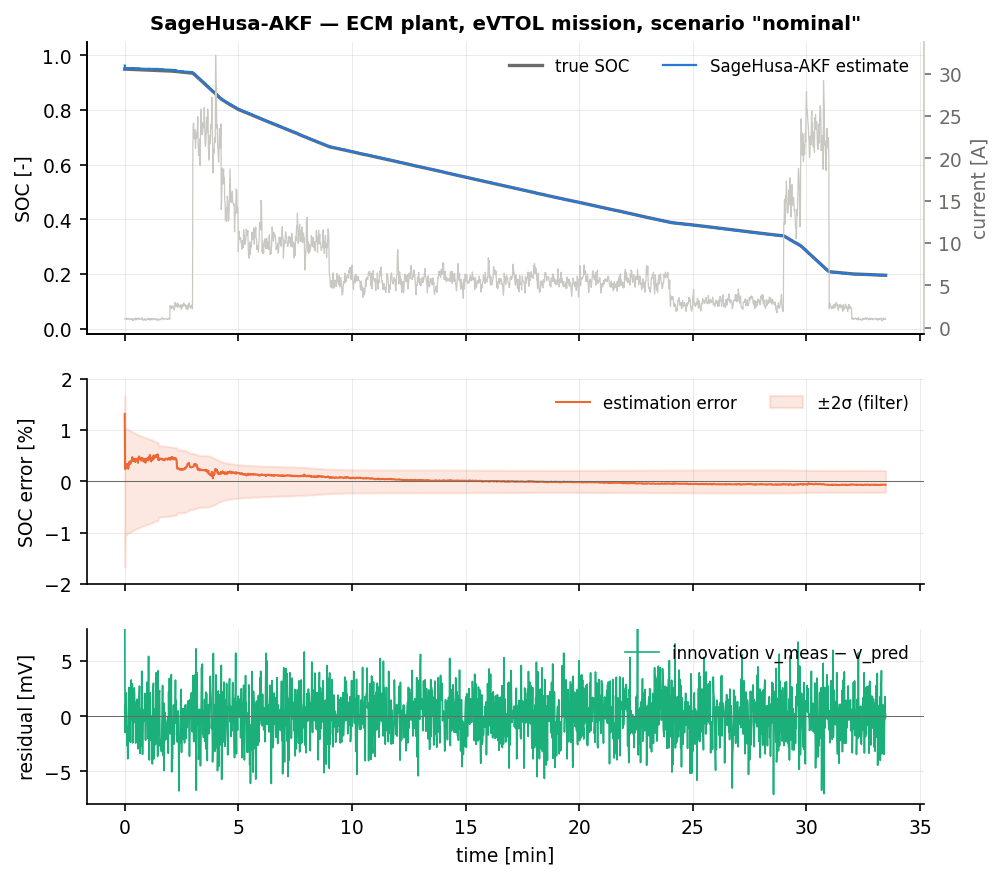
\includegraphics[width=\textwidth]{figures/cell_SageHusaAKF_nominal.png}
\caption{SageHusa-AKF on the nominal eVTOL mission: true and estimated SOC (top), estimation error with the $\pm 2\sigma$ band when available (middle), voltage residual (bottom).}
\end{figure}
\begin{figure}[H]\centering
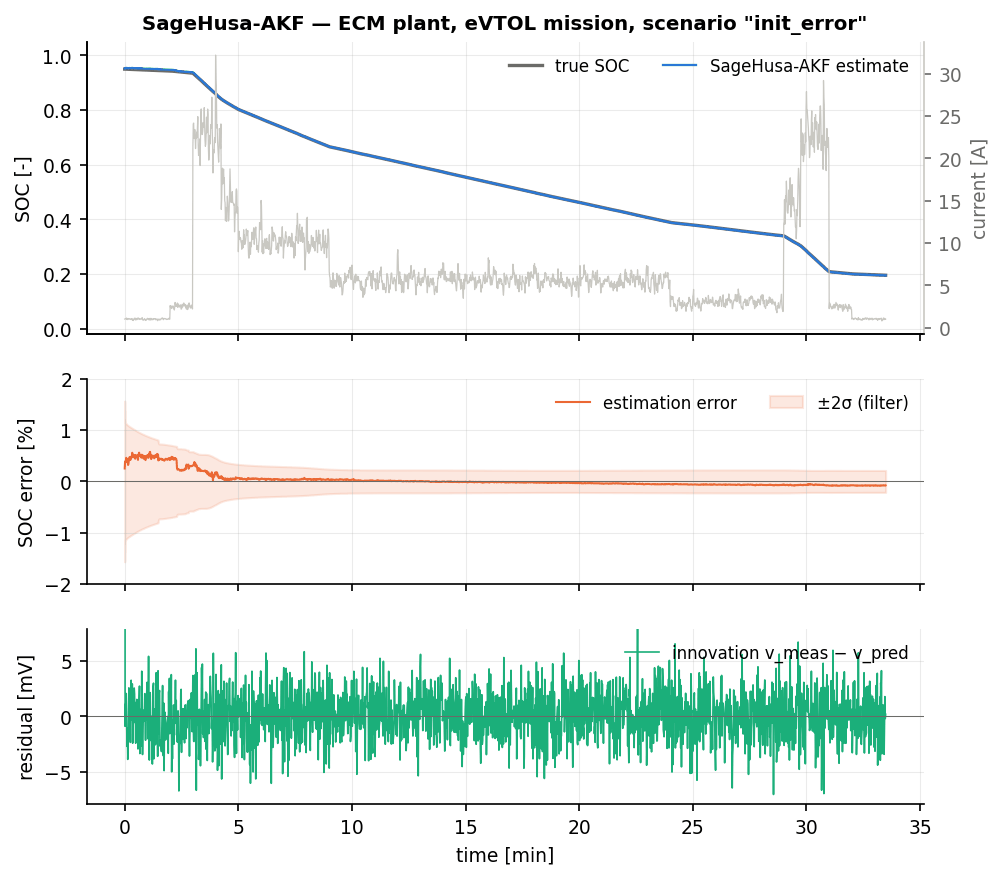
\includegraphics[width=\textwidth]{figures/cell_SageHusaAKF_init_error.png}
\caption{SageHusa-AKF with a 35\,\% initial SOC error.}
\end{figure}
\begin{figure}[H]\centering
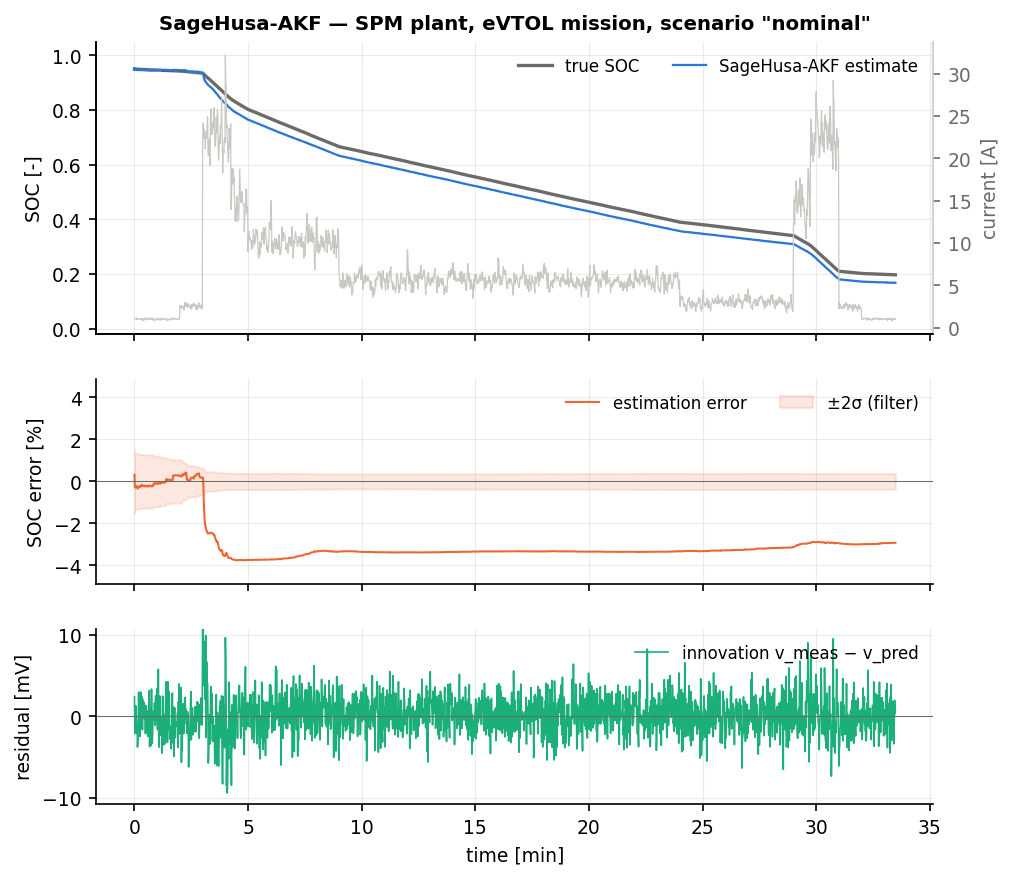
\includegraphics[width=\textwidth]{figures/cellspm_SageHusaAKF_nominal.png}
\caption{SageHusa-AKF on the electrochemical (single-particle) plant, nominal mission: the estimator uses a 2-RC ECM fitted to that plant and therefore sees a structured \SI{4}{\milli\volt} residual instead of white noise.}
\end{figure}

All figures below are three-seed means in \% SOC, as tabulated above; the plain \texttt{EKF} run on
the same data is the reference (\texttt{EKF ref.} column).  For orientation, the EKF scores
$\mathrm{rmse}_{ss}$ = 0.05\,\% on \texttt{nominal}, 0.12\,\% on \texttt{noise\_step}, 0.21\,\% on
\texttt{outliers}, 0.46\,\% on \texttt{sensor\_dropout}, 1.36\,\% on \texttt{param\_mismatch},
1.52\,\% on \texttt{aged\_cell} and 12.44\,\% on \texttt{combined} (where it never converges), and
3.73\,\% on the nominal SPM mission.

\paragraph{Benign scenarios.}  On \texttt{nominal} the filter matches the EKF and is marginally
better in steady state: $\mathrm{rmse}=0.24\,\%$, $\mathrm{rmse}_{ss}=\mathbf{0.04\,\%}$ against the
EKF's $0.15\,\%$ / $0.05\,\%$, both far inside the $2\,\%$ acceptance bound.  This is the expected
behaviour --- when the assumed $\mR$ is already correct, $\hat{\mR}_k$ fluctuates by $\pm10\,\%$
around it and the gain is unchanged.  On \texttt{init\_error} (35\,\% initial SOC error) the filter
converges within the first sample ($t_\mathrm{conv}=\SI{0}{\second}$, $\mathrm{rmse}=0.13\,\%$
against the EKF's $0.14\,\%$, maximum error $0.63\,\%$): the large prior covariance
$P_{0,\soc\soc}=\sigma_{z0}^2=0.01$ makes the first correction essentially a direct OCV inversion,
and the warm-up window prevents the corresponding \SI{30}{\milli\volt} residual from contaminating
$\hat{\mR}$.

\paragraph{Target scenario \texttt{noise\_step}.}  The voltage-sensor noise steps from
\SI{2}{\milli\volt} to \SI{20}{\milli\volt} at $t=\SI{600}{\second}$.  Measured on seed 1 and
averaged over $t\in[100,600)\,\si{\second}$ the filter reports
$\hat\sigma_v=\SI{2.17}{\milli\volt}$; over $t\in[700,2010]\,\si{\second}$ it reports
$\hat\sigma_v=\SI{19.99}{\milli\volt}$.  The identification is therefore essentially exact, and it
buys accuracy as well as consistency.  The EKF's steady-state SOC error rises from $0.05\,\%$ on
\texttt{nominal} to $0.12\,\%$ here, i.e.\ the tenfold sensor noise does leak into its SOC estimate
through a gain that is a factor $\sqrt{92}$ too large; the adaptive filter removes that leak
completely and returns to $\mathbf{0.04\,\%}$, a $3.0\times$ reduction.  Consistency is restored at
the same time: the normalised innovation squared $\mathrm{NIS}_k=\bm{e}_k^\T\mS_k\inv\bm{e}_k$, which
must average $n_y=1$ for a consistent filter, is $1.000$ before and $1.006$ after the step, whereas
the non-adaptive EKF goes from $1.099$ to $\mathbf{90.3}$ --- its innovations are a factor of
$\sqrt{90}\approx9.5$ larger than it believes, which would trip any residual-based fault monitor.
The voltage-prediction error falls accordingly, $\mathrm{rmse}_v$ from \SI{2.89}{\milli\volt} to
\SI{1.01}{\milli\volt}.

\paragraph{Where it wins on SOC.}  Adaptation pays wherever the innovations are inflated by something
the model cannot represent.  \texttt{sensor\_dropout} (the voltage reading freezes for
\SI{15}{\second} from $t=\SI{200}{\second}$): $\mathrm{rmse}$ $0.72\to0.23\,\%$ and
$\mathrm{rmse}_{ss}$ $0.46\to0.08\,\%$, factors of $3.1$ and $5.8$ --- the frozen sample stream
inflates the residuals, $\hat{\mR}$ grows, the gain collapses, and the filter coasts on coulomb
counting until the sensor recovers.  \texttt{param\_mismatch} ($R_0\times0.7$, $R_1\times1.3$,
$\tau_2\times1.5$): $1.28\to0.59\,\%$ and $1.36\to0.76\,\%$.  \texttt{outliers}:
$0.52\to0.22\,\%$ and $0.21\to0.06\,\%$ ($3.5\times$).  \texttt{aged\_cell}: $1.18\to1.07\,\%$ and
$1.52\to1.30\,\%$.  The largest effect is on \texttt{combined} (25\,\% initial SOC error,
\SI{150}{\milli\ampere} current bias, 2\,\% gain error, 10\,\% capacity loss), where the EKF
\emph{never} converges to the $2\,\%$ band ($t_\mathrm{conv}=$ --, $\mathrm{rmse}=16.02\,\%$,
$\mathrm{rmse}_{ss}=12.44\,\%$) while the Sage--Husa filter converges at $t=\SI{1446}{\second}$ with
$\mathrm{rmse}=4.95\,\%$ and $\mathrm{rmse}_{ss}=\mathbf{1.98\,\%}$ --- a $3.2\times$ and
$6.3\times$ reduction.  The mechanism is not the one the method was designed for: in
\texttt{combined} the cell's series resistance has grown to $1.25\,R_0$, which at the
\SI{5.5}{\ampere} cruise current is a \SI{16}{\milli\volt} bias on the predicted voltage; because the
NMC OCV curve is very flat near $\soc=0.9$ ($\partial\ocv/\partial\soc\approx\SI{0.2}{\volt}$ per
unit SOC), the EKF converts that bias into a $12\,\%$ SOC error.  Sage--Husa sees the bias as excess
measurement noise, inflates $\hat{\mR}$, and lets coulomb counting dominate --- which on this
scenario is the more accurate of the two information sources.

\paragraph{Costs and neutral cases.}  De-weighting the voltage channel is not free: $\mathrm{rmse}_v$
rises from \SI{3.80}{\milli\volt} to \SI{21.77}{\milli\volt} on \texttt{aged\_cell} and from
\SI{5.15}{\milli\volt} to \SI{13.91}{\milli\volt} on \texttt{combined}, because the filter
deliberately stops following a measurement it has decided is unreliable.  If the application needs an
accurate terminal-voltage prediction (for a power-limit computation, say) $\hat{\mR}$ must not be
allowed to grow without bound; \texttt{r\_max\_scale} is the knob.  On \texttt{cold}
($T=\SI{-10}{\celsius}$) the filter is slightly worse than the EKF ($0.22\,\%$ against $0.16\,\%$):
at low temperature the RC dynamics are slow, the residual sequence is strongly coloured, and that
violates \cref{as:sh:slow} and biases $\hat{\mR}$ upward.  On \texttt{preisach} --- the truth plant
uses a Preisach hysteresis operator with the corrected sign convention that the estimator does not
model --- the filter matches the EKF in steady state ($0.20\,\%$ for both) and is marginally worse
over the full run ($0.67\,\%$ against $0.58\,\%$), but it does reach the $2\,\%$ band immediately
($t_\mathrm{conv}=\SI{0}{\second}$ against the EKF's \SI{16}{\second}).  \texttt{current\_bias} is a
draw ($0.62\,\%$ against $0.61\,\%$): a constant current-sensor offset does not inflate the
innovations enough to trigger adaptation, and no amount of $\mR$ tuning can recover an input error.
Runtime is \SI{545}{\nano\second}/step against the EKF's \SI{478}{\nano\second}/step.

\paragraph{Electrochemical (SPM) plant.}  The SPM rows are the hard test: the estimator runs a 2-RC
ECM fitted to a single-particle model with Butler--Volmer kinetics and solid-diffusion time constant
$\tau\approx\SI{556}{\second}$, so the voltage residual is not white noise at all but a structured,
slowly varying \SI{4}{\milli\volt} signal.  Sage--Husa ends at $\mathrm{rmse}_{ss}=3.33\,\%$ on the
nominal SPM mission against the EKF's $3.73\,\%$ --- an improvement of barely $10\,\%$, and two
orders of magnitude worse than what the covariance-inflating filters achieve on the same data
(Fading-EKF $0.36\,\%$, STF $0.66\,\%$, \cref{ch:fadingekf} and \cref{ch:stf}).  The reason is
structural and is worth stating precisely, because it is the sharpest illustration in this chapter
of what covariance matching can and cannot do.  The recursion \eqref{eq:sh:Rrec} sees residuals that
are twice the nominal $\sigma_v$ and, being unable to ask \emph{why}, does the only thing it knows:
it raises $\hat{\mR}$ to about $(\SI{4}{\milli\volt})^2$ and lowers the Kalman gain.  Lowering the
gain hands the SOC estimate over to the coulomb integrator --- but on the SPM plant the integrator is
precisely the part that is wrong, because the fitted $Q_\mathrm{Ah}$ and coulombic efficiency do not
reproduce the true lithium inventory, so the estimate drifts to a $3\,\%$ offset and stays there.
The measurement, by contrast, is trustworthy: the ECM's static $\ocv(\soc)$ map \emph{was} fitted to
this plant, so the voltage still identifies SOC to a few tenths of a percent; what the ECM cannot
reproduce is the \emph{dynamics}.  Trusting the measurement more (inflating $\mP$) is therefore the
correct response and trusting it less (inflating $\mR$) is the wrong one, which is the exact mirror
image of the ECM \texttt{aged\_cell} result above, where the model error sat in the output equation
and inflating $\mR$ was right.  Where the SPM scenario adds an error \emph{on top of} the structural
one, the adaptation does earn its keep: \texttt{cold} $7.35\to2.65\,\%$ (a $2.8\times$ improvement,
the largest on the SPM plant) and \texttt{param\_mismatch} $3.13\to1.13\,\%$.  It is worse than the
EKF only on SPM \texttt{outliers} ($3.19\,\%$ against $1.99\,\%$), where inflating $\mR$ on top of an
already-conservative gain locks the estimate onto the drifting integrator.

\section{Summary}
The Sage--Husa filter is the cheapest useful adaptive Kalman filter: one extra output evaluation,
one $n_y\times n_y$ recursion, no inversion, no buffer.  Use it whenever the effective
measurement-noise level of a channel is uncertain or time-varying and you need the filter's
innovations to stay statistically consistent --- on this benchmark it tracks a tenfold voltage-noise
step to within $0.1\,\%$, holds $\overline{\mathrm{NIS}}\approx 1$ where the EKF reaches $90$, and
cuts the steady-state SOC error on that step from $0.12\,\%$ to $0.04\,\%$.
Do not use the $\mQ$ recursion: it is not identifiable jointly with $\mR$ and loses positive
definiteness.  Do not expect it to help when the residuals are inflated by structured model error rather than by
noise: on the electrochemical plant it improves on the EKF by barely $10\,\%$ ($3.33\,\%$ against
$3.73\,\%$) where the covariance-inflating filters reach $0.36\,\%$, because lowering the gain is
the wrong response when the model, not the sensor, is the unreliable component.  It cannot
distinguish a noisy sensor from a wrong model --- when the two must be told apart, use the IMM
(\cref{ch:imm}) instead.

% Copyright 2026 Sreeram Anil
% SPDX-License-Identifier: CC-BY-4.0
% =============================================================================
%  Innovation-based adaptive estimation (windowed covariance matching)
% =============================================================================
\chapter{Innovation-based adaptive estimation (IAE-AKF)}
\label{ch:iaeakf}

\section*{At a glance}
\begin{tabular}{@{}l>{\raggedright\arraybackslash}p{0.76\textwidth}@{}}
Family & Adaptive Kalman \\
Header & \texttt{include/estkit/filters/iae\_akf.hpp} \\
Registered name & \texttt{IAE-AKF} \\
State dimension & $n_x = 4$ (cell model) --- generic in $n_x, n_u, n_y$; window $N$ is a template parameter \\
Cost per step & EKF $+\,\mathcal{O}(n_y^2)$; $\approx 500$\,ns/step measured; $N n_y$ reals of buffer, no heap \\
Primary references & \cite{mehra1970,mohamed1999adaptive,maybeck1979,jazwinski1970} \\
\end{tabular}

\section{Motivation and aerospace/BMS relevance}
Mehra's 1970 paper \cite{mehra1970} is the origin of the whole family of adaptive Kalman filters
that work by \emph{covariance matching}.  The observation is elementary and powerful: a Kalman
filter publishes, at every step, a prediction of the second-order statistics of its own innovation
sequence, $\mS_k = \mH_k\Pminus_k\mH_k^\T + \mR_k$.  If the filter's noise model is right, the
empirical covariance of the innovations must match $\mS_k$; if it does not, the mismatch tells us
by how much, and in which direction, the model is wrong.  Mehra showed that for a linear
time-invariant system the full autocorrelation function of the innovations identifies both $\mQ$
and $\mR$ (up to the well-known identifiability restrictions), and that the zero-lag term alone
identifies $\mR$ directly.

Mohamed and Schwarz \cite{mohamed1999adaptive} turned this into the standard practical recipe used
throughout navigation: estimate the innovation covariance over a \emph{moving window} of the last
$N$ samples and subtract the part the filter attributes to state uncertainty.  Their paper calls
the resulting estimator IAE (innovation-based adaptive estimation), distinguishing it from RAE
(residual-based adaptive estimation), which uses the a-posteriori residual instead.  IAE became the
workhorse of loosely coupled INS/GPS integration, where the GPS pseudo-range noise varies by an
order of magnitude between open sky and urban canyon; the battery analogue is a cell-voltage
channel whose effective noise changes with the switching state of the traction inverter, or a
voltage multiplexer that intermittently returns a stale sample.

Compared with the Sage--Husa recursion of \cref{ch:sagehusaakf}, the windowed estimator has a
sharper time--variance trade-off: a rectangular window of length $N$ forgets completely after $N$
samples instead of exponentially, so the response to a step change in the noise level is a ramp of
exactly $N$ samples rather than an exponential tail.  It costs $N n_y$ reals of ring buffer.

\section{Problem statement and assumptions}
The plant is \eqref{eq:sh:proc}--\eqref{eq:sh:meas} of \cref{ch:sagehusaakf}.  Define the
a-priori innovation
\begin{equation}
\bm{e}_k \triangleq \vy_k - h(\xminus_k,\vu_k) \in \real^{n_y},
\label{eq:iae:innov}
\end{equation}
where $\xminus_k$ is the one-step prediction of the state.  We seek $\hat{\mR}_k$ under

\begin{assumption}\label{as:iae:white}
The filter is close enough to consistency that $\bm{e}_k$ is approximately zero-mean and white; then
$\E{\bm{e}_k\bm{e}_k^\T} = \mH_k\Pminus_k\mH_k^\T + \mR_k$.
\end{assumption}
\begin{assumption}\label{as:iae:stat}
$\mR_k$ and $\mH_k\Pminus_k\mH_k^\T$ are approximately constant over the window
$\{k-N+1,\dots,k\}$.
\end{assumption}

\section{Derivation}

\subsection{Innovation covariance and the matching condition}
For the linearised filter, propagate the estimation error $\tilde{\vx}^-_k = \vx_k - \xminus_k$:
\begin{equation}
\bm{e}_k = \vy_k - h(\xminus_k,\vu_k) = \mH_k\tilde{\vx}^-_k + \vv_k + \mathcal{O}(\|\tilde{\vx}^-_k\|^2).
\label{eq:iae:elin}
\end{equation}
$\vv_k$ is independent of $\tilde{\vx}^-_k$ (which depends only on data up to $k-1$ and on
$\vw_{0:k-1}$), so
\begin{equation}
\mC_{v,k} \triangleq \E{\bm{e}_k\bm{e}_k^\T} = \mH_k\,\E{\tilde{\vx}^-_k\tilde{\vx}^{-\T}_k}\,\mH_k^\T + \mR_k
= \mH_k\Pminus_k\mH_k^\T + \mR_k ,
\label{eq:iae:match}
\end{equation}
provided the filter's $\Pminus_k$ equals the true prediction-error covariance.  Equation
\eqref{eq:iae:match} is the \emph{covariance-matching condition}.  Solving it for $\mR_k$,
\begin{equation}
\boxed{\;\hat{\mR}_k = \hat{\mC}_{v,k} - \mH_k\Pminus_k\mH_k^\T\;}
\label{eq:iae:R}
\end{equation}
with the sample estimate over the moving window
\begin{equation}
\hat{\mC}_{v,k} = \frac{1}{N}\sum_{j=k-N+1}^{k} \bm{e}_j\bm{e}_j^\T .
\label{eq:iae:Cv}
\end{equation}
This is Mohamed and Schwarz's IAE \cite[Eq.~(16)]{mohamed1999adaptive}; Mehra
\cite[Sec.~III]{mehra1970} derives the same expression as the zero-lag element of the innovation
autocorrelation sequence.

\subsection{Statistical properties}
Under \cref{as:iae:white} and \cref{as:iae:stat} the estimator \eqref{eq:iae:R} is unbiased:
$\E{\hat{\mR}_k} = \mC_{v,k} - \mH_k\Pminus_k\mH_k^\T = \mR_k$.  Its variance follows from the
Wishart distribution of \eqref{eq:iae:Cv}: for $n_y=1$,
\begin{equation}
\frac{\Var{\hat{R}_k}}{\big(\mH_k\Pminus_k\mH_k^\T+R_k\big)^2} = \frac{2}{N},
\label{eq:iae:var}
\end{equation}
i.e.\ a relative standard deviation of $\sqrt{2/N}$ on the \emph{innovation} variance, which is
inflated by the factor $(1 + \mH\Pminus\mH^\T/R)^2$ when referred to $\hat R$ itself.  With $N=80$
the relative error is $16\,\%$; the response time to a step change in the noise level is exactly
$N$ samples.  Choosing $N$ is therefore the same bias--variance compromise as choosing $b$ in
Sage--Husa, with $N \leftrightarrow 2/(1-b)$ giving comparable variance.

\subsection{Positive definiteness}
The difference in \eqref{eq:iae:R} is not guaranteed positive definite: when the true $\mR$ is small
compared with the state-uncertainty contribution, or when the window happens to contain unusually
small innovations, $\hat{\mR}_k$ can have non-positive diagonal entries.  The standard remedy, and
the one implemented here, is a projection onto a bounded positive-definite set,
\begin{equation}
\hat R_{k,ii} \gets \mathrm{clamp}\!\left(\hat R_{k,ii},\; \rho_{\min} R_{ii},\; \rho_{\max} R_{ii}\right),
\qquad
|\hat R_{k,ij}| \le 0.99\sqrt{\hat R_{k,ii}\hat R_{k,jj}},
\label{eq:iae:floor}
\end{equation}
where $R_{ii}$ is the nominal model value.  The second condition enforces the Cauchy--Schwarz bound
on the off-diagonal entries, which for $n_y\le 2$ is sufficient for positive definiteness and for
larger $n_y$ is a cheap necessary condition.  For the cell model $n_y=1$ and only the clamp acts.

\subsection{Why the process-noise covariance is not adapted}
The companion IAE estimator for the process noise,
$\hat{\mQ}_k = \hat{\mC}_{\Delta x,k} + \Pplus_k - \mF_{k-1}\Pplus_{k-1}\mF_{k-1}^\T$ with
$\hat{\mC}_{\Delta x,k}$ the windowed covariance of the state correction $\mK_j\bm{e}_j$
\cite[Eq.~(17)]{mohamed1999adaptive}, requires $N \gg n_x^2$ samples to be usable and, like the
Sage--Husa version, suffers from the fundamental non-identifiability of $(\mQ,\mR)$ from a single
output record \cite{mehra1970}: only $n_y(n_y+1)/2 \cdot n_x$ elements of the autocorrelation
sequence are informative, which is generally fewer than the $n_x(n_x+1)/2$ unknowns in $\mQ$.  For
the ECM, $\mQ$ is moreover structured (it is the image of the current-sensor noise through
$\partial f/\partial i$ plus a diagonal floor), so an unstructured estimate would discard known
information.  $\mQ$ adaptation is therefore not offered.

\section{Algorithm}
\begin{algorithm}[H]
\caption{IAE-AKF --- one sampling period}
\begin{algorithmic}[1]
\Require $\xplus_{k-1},\Pplus_{k-1},\vu_{k-1},\vy_k,\vu_k$, ring buffer $\{\bm{e}_{k-N},\dots,\bm{e}_{k-1}\}$, running sum $\Sigma$
\State \textbf{Time update:} $\xminus_k\gets f(\xplus_{k-1},\vu_{k-1})$;\quad
       $\Pminus_k\gets\mF\Pplus_{k-1}\mF^\T+\mQ_k$
\State \textbf{Innovation:} $\mH\gets\partial h/\partial\vx|_{\xminus_k}$;\quad $\bm{e}_k\gets\vy_k-h(\xminus_k,\vu_k)$
\State \textbf{Ring buffer:} if full, $\Sigma\gets\Sigma-\bm{e}_{k-N}\bm{e}_{k-N}^\T$;\quad
       store $\bm{e}_k$;\quad $\Sigma\gets\Sigma+\bm{e}_k\bm{e}_k^\T$
\State \textbf{Covariance matching} (if buffer has $\ge N_{\min}$ entries):
       $\hat{\mC}_v\gets\Sigma/n$;\quad $\hat{\mR}_k\gets\hat{\mC}_v-\mH\Pminus_k\mH^\T$;\quad apply \eqref{eq:iae:floor}
\State \textbf{Gain:} $\mS_k\gets\mH\Pminus_k\mH^\T+\hat{\mR}_k$;\quad $\mK_k\gets\Pminus_k\mH^\T\mS_k\inv$
\State \textbf{State update:} $\xplus_k\gets\xminus_k+\mK_k\bm{e}_k$
\State \textbf{Covariance (Joseph):} $\Pplus_k\gets(\mI-\mK_k\mH)\Pminus_k(\mI-\mK_k\mH)^\T+\mK_k\hat{\mR}_k\mK_k^\T$
\State \textbf{Constrain:} $\xplus_k\gets\mathrm{constrain}(\xplus_k)$
\Ensure $\xplus_k,\Pplus_k,\hat{\mR}_k$
\end{algorithmic}
\end{algorithm}
The running sum $\Sigma$ makes the window update $\mathcal{O}(n_y^2)$ instead of
$\mathcal{O}(N n_y^2)$; the buffer is a fixed-size array, so no heap is used.  Note that
$\hat{\mR}_k$ is computed \emph{before} the gain, so the current sample already benefits from the
adaptation --- unlike the Sage--Husa recursion, which necessarily updates $\hat{\mR}$ after the
state update because it uses the a-posteriori residual.

\section{Application to the battery model}
With $n_y=1$ the estimator reduces to
$\hat R_k = \frac{1}{N}\sum_j e_j^2 - \big(\partial\ocv/\partial\soc\big)^2 P^-_{\soc\soc}
- \dots$, i.e.\ a plain running mean of squared voltage innovations, less the (usually tiny)
model-uncertainty contribution.  The window is a template parameter, \texttt{IaeAkf<Model, NWIN>};
the registered estimator uses $N = 80$ samples $=\SI{8}{\second}$.  The choice sits in the middle
of the $N=50$--$100$ range used in the navigation literature and was checked against $N\in\{50,100\}$:
the steady-state metrics vary by less than $20\,\%$ and the ranking against the EKF does not change.
At \SI{10}{\hertz}, $N=80$ gives a $16\,\%$ relative accuracy on the variance estimate and an
\SI{8}{\second} reaction time, which is short compared with the slow RC time constant
$\tau_2=\SI{120}{\second}$ of the cell and long compared with the fast one, $\tau_1=\SI{5}{\second}$.
The bounds are $\rho_{\min}=0.05$, $\rho_{\max}=5\times10^3$, i.e.\
$\hat\sigma_v\in[0.47,148]\,\si{\milli\volt}$; adaptation starts only once the window is full
(\texttt{min\_samples} $=N$), so the initial transient of the filter does not enter the estimate.
An optional first-order smoother on $\hat{\mR}$ (\texttt{opts.smooth}) is provided but defaults to
off.

\section{Implementation notes}
\begin{itemize}[leftmargin=1.4em]
\item \textbf{Buffer.}  \texttt{Y buf\_[NWIN]} plus one $n_y\times n_y$ running sum; for the cell
      model that is $80$ doubles $=640$\,bytes.  Wrapping is done with a single modulo on the
      head index.  Deleting the oldest outer product and adding the newest keeps the cost at
      $\mathcal{O}(n_y^2)$ per sample.
\item \textbf{Drift.}  Maintaining $\Sigma$ incrementally accumulates round-off over long runs.  For
      $n=2\times10^4$ samples in double precision this is far below the $16\,\%$ statistical error;
      in the float32 build it was verified to leave the metrics unchanged to three digits.  If a
      run of $10^7$ samples were required, periodic re-summation of the buffer would be the fix.
\item \textbf{Ordering.}  $\hat{\mR}_k$ uses $\Pminus_k$ \emph{before} the update, which is the
      quantity that appears in \eqref{eq:iae:match}.  Using $\Pplus_k$ here is a common
      implementation error and biases $\hat{\mR}$ upwards.
\item \textbf{Cold start.}  Before the window is full the filter runs with the nominal model $\mR$;
      this avoids the very noisy one- or two-sample variance estimates that a naive implementation
      would produce.
\item \textbf{Cost.}  Measured \SI{500}{\nano\second}/step against the EKF's
      \SI{478}{\nano\second}/step (a $5\,\%$ overhead).  It is the cheapest of the adaptive filters in
      this family because it needs no extra evaluation of $h$.  On a \SI{400}{\mega\hertz} Cortex-M7
      this scales to roughly \SI{6}{\micro\second}/step.
\item \textbf{Limitations.}  \cref{as:iae:white} is violated whenever the innovations are coloured,
      which happens with slow un-modelled dynamics (cold cell, hysteresis mismatch); the estimator
      then over-estimates $\mR$.  The rectangular window also means a single very large innovation
      stays in the estimate at full weight for exactly $N$ samples and then disappears abruptly,
      which produces a small step in the gain.
\end{itemize}

\section{Benchmark results}
% Copyright 2026 Sreeram Anil
% SPDX-License-Identifier: CC-BY-4.0
\begin{table}[H]\centering\footnotesize\setlength{\tabcolsep}{4pt}
\caption{IAE-AKF: cell-level benchmark on the eVTOL mission (mean over seeds; RMSE and max error in \% SOC; $t_\mathrm{conv}$: first time the error stays below 2\,\% for 60\,s, -- = never; EKF reference: steady-state RMSE of the plain EKF on the same data).}\label{tab:cell_IAEAKF}
\begin{tabular}{llrrrrrcrr}\toprule
plant & scenario & RMSE & RMSE$_\mathrm{ss}$ & max & $t_\mathrm{conv}$ [s] & RMSE$_v$ [mV] & div. & EKF ref. & ns/step \\ \midrule
ECM & nominal & 0.22 & 0.04 & 1.08 & 0 & 0.79 & no & 0.05 & 500 \\
ECM & init\_error & 0.12 & 0.07 & 0.60 & 0 & 2.12 & no & 0.05 & 499 \\
ECM & current\_bias & 0.53 & 0.62 & 1.39 & 0 & 0.87 & no & 0.61 & 499 \\
ECM & noise\_step & 0.22 & 0.04 & 1.08 & 0 & 1.01 & no & 0.12 & 499 \\
ECM & outliers & 0.41 & 0.11 & 2.92 & 2 & 1.04 & no & 0.21 & 501 \\
ECM & cold & 0.19 & 0.16 & 1.17 & 0 & 1.89 & no & 0.16 & 498 \\
ECM & hot & 0.19 & 0.03 & 1.01 & 0 & 0.54 & no & 0.03 & 499 \\
ECM & aged\_cell & 1.06 & 1.21 & 2.61 & 0 & 24.50 & no & 1.52 & 500 \\
ECM & param\_mismatch & 0.85 & 1.01 & 1.69 & 0 & 7.54 & no & 1.36 & 499 \\
ECM & sensor\_dropout & 0.20 & 0.05 & 1.08 & 0 & 0.90 & no & 0.46 & 498 \\
ECM & preisach & 0.61 & 0.20 & 1.82 & 0 & 0.81 & no & 0.20 & 500 \\
ECM & combined & 4.89 & 2.01 & 11.44 & 1448 & 16.50 & no & 12.44 & 501 \\
\midrule
SPM & nominal & 2.94 & 3.02 & 3.54 & 0 & 1.43 & no & 3.73 & 471 \\
SPM & init\_error & 3.56 & 3.56 & 4.49 & 9 & 2.42 & no & 3.81 & 469 \\
SPM & current\_bias & 4.76 & 5.45 & 6.10 & 0 & 1.71 & no & 5.69 & 470 \\
SPM & noise\_step & 2.94 & 3.02 & 3.54 & 0 & 2.30 & no & 3.30 & 473 \\
SPM & outliers & 2.58 & 2.58 & 3.91 & 0 & 2.30 & no & 1.99 & 475 \\
SPM & cold & 2.70 & 2.54 & 3.58 & 0 & 18.15 & no & 7.35 & 466 \\
SPM & hot & 2.13 & 2.19 & 2.53 & 0 & 0.75 & no & 2.16 & 472 \\
SPM & param\_mismatch & 1.14 & 1.20 & 2.00 & 0 & 4.47 & no & 3.13 & 469 \\
SPM & sensor\_dropout & 3.12 & 3.19 & 3.79 & 0 & 2.09 & no & 5.31 & 472 \\
\bottomrule\end{tabular}\end{table}

\begin{figure}[H]\centering
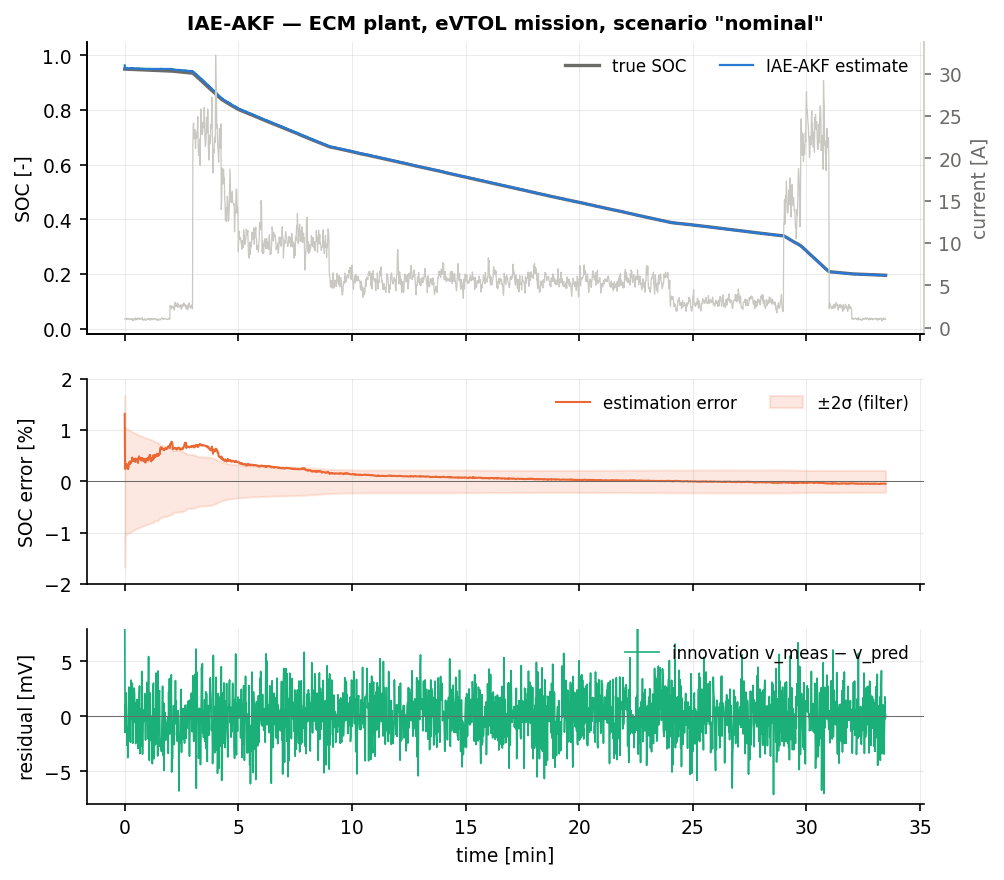
\includegraphics[width=\textwidth]{figures/cell_IAEAKF_nominal.png}
\caption{IAE-AKF on the nominal eVTOL mission: true and estimated SOC (top), estimation error with the $\pm 2\sigma$ band when available (middle), voltage residual (bottom).}
\end{figure}
\begin{figure}[H]\centering
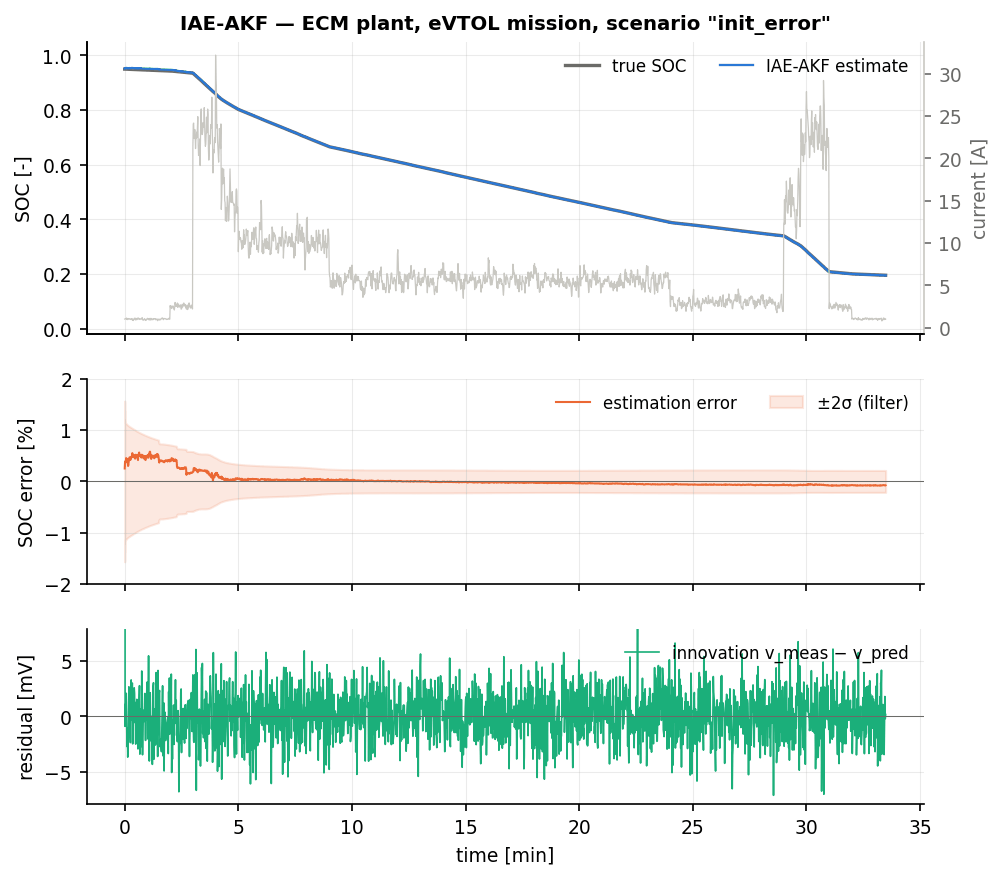
\includegraphics[width=\textwidth]{figures/cell_IAEAKF_init_error.png}
\caption{IAE-AKF with a 35\,\% initial SOC error.}
\end{figure}
\begin{figure}[H]\centering
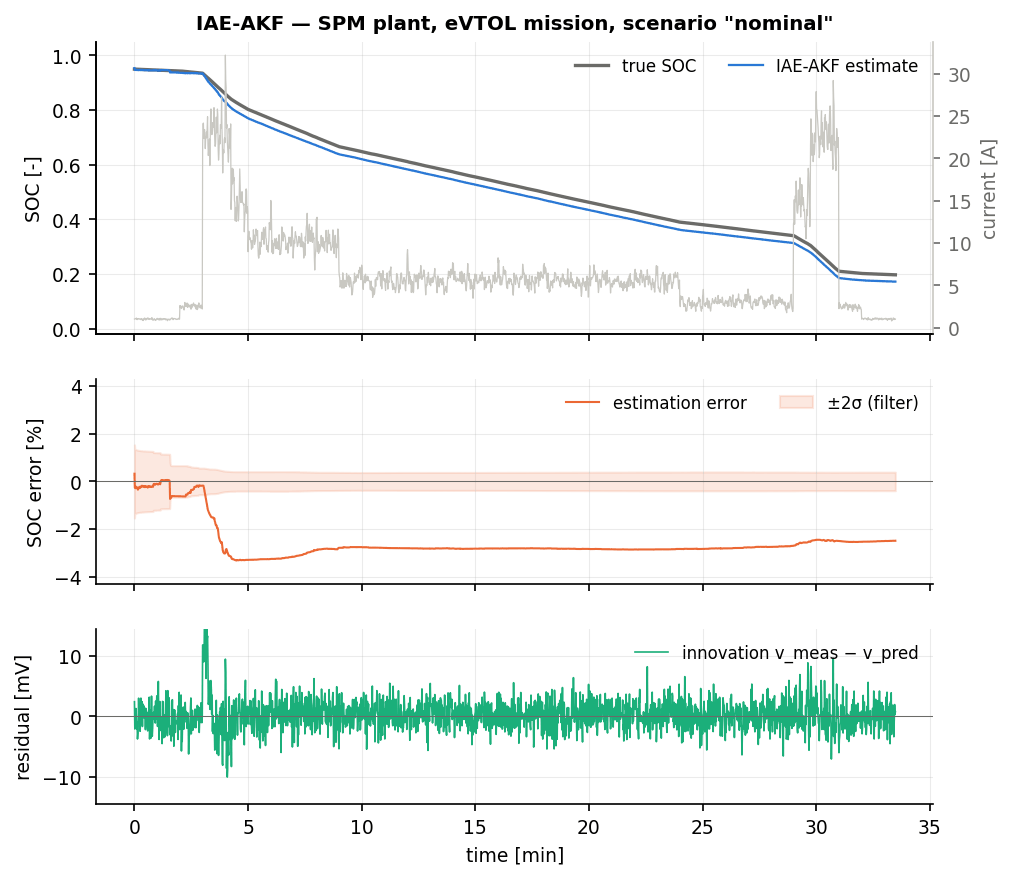
\includegraphics[width=\textwidth]{figures/cellspm_IAEAKF_nominal.png}
\caption{IAE-AKF on the electrochemical (single-particle) plant, nominal mission: the estimator uses a 2-RC ECM fitted to that plant and therefore sees a structured \SI{4}{\milli\volt} residual instead of white noise.}
\end{figure}

All figures below are three-seed means in \% SOC, as tabulated above; the plain \texttt{EKF} run on
the same data is the reference (\texttt{EKF ref.} column).  For orientation, the EKF scores
$\mathrm{rmse}_{ss}$ = 0.05\,\% on \texttt{nominal}, 0.12\,\% on \texttt{noise\_step}, 0.21\,\% on
\texttt{outliers}, 0.46\,\% on \texttt{sensor\_dropout}, 1.36\,\% on \texttt{param\_mismatch},
1.52\,\% on \texttt{aged\_cell} and 12.44\,\% on \texttt{combined} (where it never converges), and
3.73\,\% on the nominal SPM mission.

\paragraph{Benign scenarios.}  \texttt{nominal}: $\mathrm{rmse}=0.22\,\%$,
$\mathrm{rmse}_{ss}=\mathbf{0.04\,\%}$ against the EKF's $0.15\,\%$ / $0.05\,\%$.  The adaptation is
inactive in the useful sense --- $\hat\sigma_v$ hovers at \SI{2.15}{\milli\volt} against the nominal
\SI{2.13}{\milli\volt} --- and the filter is a plain EKF.  \texttt{init\_error}: converges at
$t=\SI{0}{\second}$ with $\mathrm{rmse}=0.12\,\%$ and $\mathrm{rmse}_{ss}=0.07\,\%$ (EKF $0.14\,\%$ /
$0.05\,\%$); the slightly larger steady-state value comes from the first $N$ samples, during which the
window fills with the very large innovations of the initial transient and $\hat{\mR}$ is briefly
inflated.  Both are far inside the $2\,\%$ acceptance bound.

\paragraph{Target scenario \texttt{noise\_step}.}  The estimated voltage-noise standard deviation
(seed 1) averages \SI{2.15}{\milli\volt} over $t\in[100,600)\,\si{\second}$ and
\SI{19.94}{\milli\volt} over $t\in[700,2010]\,\si{\second}$ --- within $0.3\,\%$ of the true
\SI{2}{\milli\volt}\,$\to$\,\SI{20}{\milli\volt} step once the \SI{0.6}{\milli\volt} contribution of
the current-sensor noise through $R_0$ is accounted for.  The SOC benefit is now unambiguous: the
EKF's steady-state error rises from $0.05\,\%$ on \texttt{nominal} to $0.12\,\%$ here because its
gain is a factor $\sqrt{92}$ too large for the new noise level, whereas IAE returns to
$\mathbf{0.04\,\%}$ --- a $3.0\times$ reduction, and the joint best of this family together with
Sage--Husa.  Consistency is restored exactly: the mean normalised innovation squared is $1.000$ both
before and after the step, against $1.099$ and $\mathbf{90.3}$ for the EKF.  The voltage-prediction
error falls from \SI{2.89}{\milli\volt} to \SI{1.01}{\milli\volt}, the best of all eight estimators in
this family.

\paragraph{Fault de-weighting.}  The clearest SOC benefit is on \texttt{sensor\_dropout}, where the
voltage reading is frozen at its value at $t=\SI{200}{\second}$ for \SI{15}{\second}.  The window
estimate reacts inside the fault: $\hat\sigma_v$ averages \SI{2.14}{\milli\volt} over
$[100,200)\,\si{\second}$, \SI{18.9}{\milli\volt} \emph{during} $[200,215)\,\si{\second}$ and
\SI{2.71}{\milli\volt} over $[215,400)\,\si{\second}$ --- an automatic, un-tuned nine-fold
de-weighting of a stuck sensor followed by a clean recovery.  The resulting metrics are
$\mathrm{rmse}=0.20\,\%$ and $\mathrm{rmse}_{ss}=\mathbf{0.05\,\%}$ against the EKF's $0.72\,\%$ and
$0.46\,\%$, improvements of $3.6\times$ and $9.2\times$ and the joint best of the whole family on this
scenario.  On \texttt{outliers} (5\,\% of samples corrupted by $\pm\SI{50}{\milli\volt}$) the filter
settles at $\hat\sigma_v=\SI{11.1}{\milli\volt}$ --- exactly the standard deviation of the
contaminated distribution --- and improves $\mathrm{rmse}$ from $0.52\,\%$ to $0.41\,\%$ and
$\mathrm{rmse}_{ss}$ from $0.21\,\%$ to $0.11\,\%$.  That is a real but modest gain: a uniformly
inflated $\mR$ is a blunt instrument against impulsive noise, and the variational filter of
\cref{ch:vbakf}, which reweights \emph{within} the sample, reaches $0.05\,\%$.

\paragraph{Model mismatch.}  \texttt{param\_mismatch}: $\mathrm{rmse}$ $1.28\to0.85\,\%$,
$\mathrm{rmse}_{ss}$ $1.36\to1.01\,\%$.  \texttt{aged\_cell}: $1.18\to1.06\,\%$,
$1.52\to1.21\,\%$.  \texttt{combined}: the EKF never reaches the $2\,\%$ band
($t_\mathrm{conv}=$ --, $16.02\,\%$ / $12.44\,\%$); the IAE filter converges at
$t=\SI{1448}{\second}$ with $4.89\,\%$ / $\mathbf{2.01\,\%}$, a $3.3\times$ / $6.2\times$
improvement.  The mechanism is the one analysed in \cref{ch:sagehusaakf}: the grown series
resistance puts a \SI{16}{\milli\volt} bias on the predicted voltage, the covariance-matching
estimator reads that bias as measurement noise, and the resulting de-weighting of the voltage channel
is the right thing to do for SOC because coulomb counting is the more trustworthy source on that
scenario.  The price is the voltage prediction, $\mathrm{rmse}_v$ rising from \SI{5.15}{\milli\volt}
to \SI{16.50}{\milli\volt} on \texttt{combined} and from \SI{3.80}{\milli\volt} to
\SI{24.50}{\milli\volt} on \texttt{aged\_cell} --- the largest voltage-prediction penalty in the
family, a direct consequence of the rectangular window's willingness to push $\hat{\mR}$ to its
ceiling.  \texttt{preisach} (Preisach hysteresis in the truth plant, corrected sign convention):
$0.61\,\%$ / $0.20\,\%$ against the EKF's $0.58\,\%$ / $0.20\,\%$ --- a draw in steady state, with
immediate convergence against the EKF's \SI{16}{\second}.  \texttt{cold} is also a draw
($0.16\,\%$ for both) and \texttt{current\_bias} is unchanged ($0.62\,\%$ against $0.61\,\%$), as it
must be: an input-side error does not inflate the innovations.

\paragraph{Comparison with Sage--Husa.}  The two estimators are within a few percent of each other on
almost every scenario, as the theory predicts --- they are the same covariance-matching idea with a
rectangular versus an exponential window.  IAE is faster (\SI{500}{\nano\second} against
\SI{545}{\nano\second}/step, both against the EKF's \SI{478}{\nano\second}), reacts to a fault
\emph{during} the fault rather than after it (because it adapts before the gain is formed), and is
better on \texttt{sensor\_dropout} ($0.05\,\%$ against $0.08\,\%$); Sage--Husa needs no buffer, is
structurally positive definite, and is better on \texttt{param\_mismatch} ($0.76\,\%$ against
$1.01\,\%$) and \texttt{outliers} ($0.06\,\%$ against $0.11\,\%$).

\paragraph{Electrochemical (SPM) plant.}  On the single-particle plant the estimator runs a 2-RC ECM
fitted to an electrochemical model with Butler--Volmer kinetics and a solid-diffusion time constant
of \SI{556}{\second}; the residual is therefore not white noise but a structured, slowly varying
\SI{4}{\milli\volt} signal.  IAE reaches $\mathrm{rmse}_{ss}=3.02\,\%$ on the nominal SPM mission
against the EKF's $3.73\,\%$ --- an $19\,\%$ improvement, and the best of the four $\mR$-adapting
filters, but far behind the covariance-inflating ones (Fading-EKF $0.36\,\%$, STF $0.66\,\%$).
Equation \eqref{eq:iae:R} is doing exactly what it was built to do and that is the problem: it
measures $\hat{\mC}_v\approx(\SI{4}{\milli\volt})^2$, subtracts the negligible
$\mH\Pminus\mH^\T$, concludes that the voltage channel carries four millivolts of noise, and lowers
the gain.  A lower gain means the SOC estimate is produced almost entirely by the coulomb integrator
--- and on the SPM plant the integrator is the faulty component, because the fitted capacity and
efficiency do not reproduce the true lithium inventory.  The voltage, by contrast, is informative:
the ECM's $\ocv(\soc)$ map was fitted to this plant, so inverting it would locate SOC to a few tenths
of a percent.  Under \emph{structured} model error the useful response is to shorten the filter's
memory so that recent measurements dominate the accumulated model (inflate $\mP$); covariance
matching does the opposite.  Where the SPM scenario piles a further error on top, the adaptation
helps as designed: \texttt{cold} $7.35\to2.54\,\%$ ($2.9\times$) and \texttt{param\_mismatch}
$3.13\to1.20\,\%$ ($2.6\times$).  SPM \texttt{outliers} is the one regression ($2.58\,\%$ against
$1.99\,\%$).

\section{Summary}
IAE is the most direct expression of covariance matching: measure the innovation covariance, subtract
what the filter already accounts for, and call the rest measurement noise.  Use it when the
measurement-noise level is uncertain or intermittently faulty and a fixed-length reaction time is
wanted --- here it tracks a tenfold noise step to within $0.3\,\%$ and cuts the SOC RMSE on a
stuck-sensor fault by a factor of nine and the error on a tenfold noise step from $0.12\,\%$ to
$0.04\,\%$.  On the electrochemical plant, where the residual is structured rather than white, it
gains only $19\,\%$ on the EKF ($3.02\,\%$ against $3.73\,\%$) while a fading-memory filter reaches
$0.36\,\%$ --- covariance matching lowers the gain, and under model error the useful move is the
opposite.  Do not use it when the innovations are strongly coloured
(it will over-estimate $\mR$), when the disturbance is impulsive rather than Gaussian (use a robust
update), or when you need to know \emph{why} the innovations grew --- covariance matching cannot
separate a noisy sensor from a wrong model.

% Copyright 2026 Sreeram Anil
% SPDX-License-Identifier: CC-BY-4.0
% =============================================================================
%  Variational Bayesian adaptive Kalman filter (inverse-Gamma noise model)
% =============================================================================
\chapter{Variational Bayesian adaptive Kalman filter (VB-AKF)}
\label{ch:vbakf}

\section*{At a glance}
\begin{tabular}{@{}l>{\raggedright\arraybackslash}p{0.76\textwidth}@{}}
Family & Adaptive Kalman \\
Header & \texttt{include/estkit/filters/vb\_akf.hpp} \\
Registered name & \texttt{VB-AKF} \\
State dimension & $n_x = 4$ (cell model) --- generic in $n_x, n_u, n_y$ \\
Cost per step & $N_{vb}\times$ an EKF measurement update, $\mathcal{O}(N_{vb}n_x^2 n_y)$; $\approx 870$\,ns/step, no heap \\
Primary references & \cite{sarkka2009vb,sarkka2013,bishop2006prml,beal2003vb,jazwinski1970} \\
\end{tabular}

\section{Motivation and aerospace/BMS relevance}
The covariance-matching filters of \cref{ch:sagehusaakf} and \cref{ch:iaeakf} estimate the noise covariance
with a point estimate computed from a window of past innovations.  They are cheap and they work, but
they are not Bayesian: the uncertainty about $\mR$ is never represented, the state update always
uses the current best guess as if it were exact, and a single anomalous sample is averaged into the
estimate with the same weight as any other.

Särkkä and Nummenmaa \cite{sarkka2009vb} pose the problem properly.  The measurement variances are
random variables with a conjugate (inverse-Gamma) prior; the joint posterior over state and
variances is intractable, so it is approximated by the closest factorised distribution in the
Kullback--Leibler sense.  The result is a recursion that, at every sample, alternates a Kalman
update given the current variance estimate with a variance update given the current state estimate,
a handful of times.  Three properties make this attractive in a BMS.

First, the variance estimate is \emph{per channel and automatically positive}: the inverse-Gamma
parameters $\alpha,\beta$ are both positive by construction, so no floor or projection is needed to
keep $\hat{\mR}$ positive definite.  Second, because the update is iterated \emph{within} the
sample, a single large innovation is immediately reflected in a larger $\hat{\mR}$ for that very
sample, and is therefore down-weighted.  This makes VB-AKF behave like an iteratively reweighted
(Student-$t$-like) estimator and gives it genuine robustness to impulsive measurement errors --- on
this benchmark it is the best of the eight adaptive filters on the \texttt{outliers} scenario by a
factor of four.  Third, the extra cost is a small integer multiple of a measurement update, with
no buffers: on a cell-monitoring ASIC this is the difference between three and one multiply--add
sweeps over a $4\times4$ matrix.

The variational-Bayes machinery itself is standard in machine learning
\cite[Ch.~10]{bishop2006prml}\cite{beal2003vb}; \cite{sarkka2009vb} was the first recursive,
constant-cost filtering version, and it has since been extended to joint $\mQ$/$\mR$ adaptation
\cite{huang2018vbakf}.

\section{Problem statement and assumptions}
Take the plant \eqref{eq:sh:proc}--\eqref{eq:sh:meas} but model the measurement-noise covariance as
diagonal with unknown, slowly varying entries:
\begin{equation}
\vy_k = h(\vx_k,\vu_k) + \vv_k,\qquad
\vv_k\sim\N{\bm 0}{\bm{\Sigma}_k},\qquad
\bm{\Sigma}_k = \diag\!\big(\sigma^2_{k,1},\dots,\sigma^2_{k,n_y}\big).
\label{eq:vb:model}
\end{equation}
Each variance carries an independent inverse-Gamma prior,
\begin{equation}
p(\sigma^2_{k,i}) = \mathrm{Inv\text{-}Gamma}(\sigma^2_{k,i}\mid \alpha_{k,i},\beta_{k,i})
= \frac{\beta_{k,i}^{\alpha_{k,i}}}{\Gamma(\alpha_{k,i})}\,(\sigma^2_{k,i})^{-\alpha_{k,i}-1}
  \exp\!\Big(\!-\frac{\beta_{k,i}}{\sigma^2_{k,i}}\Big),
\label{eq:vb:ig}
\end{equation}
with shape $\alpha_{k,i}>0$ and scale $\beta_{k,i}>0$; recall
$\E{\sigma^{-2}} = \alpha/\beta$ and $\E{\sigma^2}=\beta/(\alpha-1)$ for $\alpha>1$.

\begin{assumption}\label{as:vb:diag}
$\bm{\Sigma}_k$ is diagonal, i.e.\ the measurement channels are independently corrupted.  (For the
cell model $n_y=1$ and the assumption is vacuous.)
\end{assumption}
\begin{assumption}\label{as:vb:fact}
The filtering posterior factorises, $p(\vx_k,\bm{\Sigma}_k\mid \vy_{1:k})\approx
Q_x(\vx_k)\,Q_\Sigma(\bm{\Sigma}_k)$.
\end{assumption}
\begin{assumption}\label{as:vb:dyn}
The variances evolve slowly; the heuristic dynamic model of \cite[Sec.~III]{sarkka2009vb},
$\alpha^-_{k,i}=\rho\,\alpha_{k-1,i}$, $\beta^-_{k,i}=\rho\,\beta_{k-1,i}$ with $\rho\in(0,1]$, is
used to spread the distribution between samples while preserving its mean.
\end{assumption}

\section{Derivation}

\subsection{The variational free energy}
Write $\bm\theta = (\vx_k,\bm\Sigma_k)$ and let $p(\bm\theta,\vy_k) = p(\vy_k\mid\bm\theta)\,
p(\vx_k\mid\vy_{1:k-1})\,p(\bm\Sigma_k\mid\vy_{1:k-1})$ be the joint one-step-ahead model.  For any
distribution $Q(\bm\theta)$,
\begin{equation}
\ln p(\vy_k) = \underbrace{\int Q(\bm\theta)\ln\frac{p(\bm\theta,\vy_k)}{Q(\bm\theta)}\,\mathrm{d}\bm\theta}_{\textstyle \mathcal{F}[Q]\ \text{(free energy)}}
\;+\; \underbrace{\mathrm{KL}\big[Q(\bm\theta)\,\|\,p(\bm\theta\mid\vy_k)\big]}_{\ \ge 0}.
\label{eq:vb:fe}
\end{equation}
Since $\ln p(\vy_k)$ does not depend on $Q$, maximising the free energy $\mathcal{F}[Q]$ is exactly
minimising the KL divergence to the true posterior.  Restricting $Q$ to the factorised family of
\cref{as:vb:fact} and taking the functional derivative of $\mathcal{F}$ with respect to each factor
under the normalisation constraint gives the classical stationarity conditions
\cite[Sec.~10.1]{bishop2006prml}
\begin{align}
\ln Q_x(\vx_k) &= \mathbb{E}_{Q_\Sigma}\!\left[\ln p(\vy_k,\vx_k,\bm\Sigma_k\mid \vy_{1:k-1})\right] + c_x,
\label{eq:vb:qx}\\
\ln Q_\Sigma(\bm\Sigma_k) &= \mathbb{E}_{Q_x}\!\left[\ln p(\vy_k,\vx_k,\bm\Sigma_k\mid \vy_{1:k-1})\right] + c_\Sigma.
\label{eq:vb:qs}
\end{align}
These are coupled --- each expectation needs the other factor --- so they are solved by cyclic
iteration, which is guaranteed to increase $\mathcal{F}$ monotonically and hence to converge to a
local maximum \cite[Sec.~10.1.1]{bishop2006prml}.

\subsection{The two factors are conjugate}
Write the joint log density.  With the prediction
$p(\vx_k\mid\vy_{1:k-1}) = \N{\xminus_k}{\Pminus_k}$, the linearised likelihood
$p(\vy_k\mid\vx_k,\bm\Sigma_k)=\N{h(\xminus_k,\vu_k)+\mH_k(\vx_k-\xminus_k)}{\bm\Sigma_k}$ and the
prior \eqref{eq:vb:ig},
\begin{multline}
\ln p(\vy_k,\vx_k,\bm\Sigma_k\mid\vy_{1:k-1}) = -\tfrac12(\vx_k-\xminus_k)^\T\Pminus_k{}\inv(\vx_k-\xminus_k)\\
-\tfrac12\sum_{i=1}^{n_y}\Big[\ln\sigma^2_{k,i} + \frac{\big(y_{k,i}-h_i(\xminus_k,\vu_k)-(\mH_k(\vx_k-\xminus_k))_i\big)^2}{\sigma^2_{k,i}}\Big]\\
-\sum_{i=1}^{n_y}\Big[(\alpha^-_{k,i}+1)\ln\sigma^2_{k,i}+\frac{\beta^-_{k,i}}{\sigma^2_{k,i}}\Big] + c .
\label{eq:vb:joint}
\end{multline}

\paragraph{State factor.}  Taking $\mathbb{E}_{Q_\Sigma}\!\left[\cdot\right]$ of \eqref{eq:vb:joint}, only
$\E{1/\sigma^2_{k,i}}=\alpha_{k,i}/\beta_{k,i}$ appears, so \eqref{eq:vb:qx} is a Gaussian
log-density with the effective noise covariance
\begin{equation}
\bm{\Sigma}^{\text{eff}} = \Big(\mathbb{E}_{Q_\Sigma}\!\left[\bm\Sigma\inv\right]\Big)\inv = \diag\!\big(\beta_{k,i}/\alpha_{k,i}\big).
\label{eq:vb:Sigeff}
\end{equation}
Completing the square gives exactly the Kalman measurement update with $\bm\Sigma^{\text{eff}}$ in
place of $\mR$:
\begin{align}
\mS^{(j)} &= \mH_k\Pminus_k\mH_k^\T + \bm\Sigma^{(j)}, \label{eq:vb:S}\\
\mK^{(j)} &= \Pminus_k\mH_k^\T\big(\mS^{(j)}\big)\inv, \label{eq:vb:K}\\
\bm m^{(j+1)} &= \xminus_k + \mK^{(j)}\big(\vy_k - h(\xminus_k,\vu_k)\big), \label{eq:vb:m}\\
\mP^{(j+1)} &= (\mI-\mK^{(j)}\mH_k)\Pminus_k(\mI-\mK^{(j)}\mH_k)^\T + \mK^{(j)}\bm\Sigma^{(j)}\mK^{(j)\T}. \label{eq:vb:P}
\end{align}

\paragraph{Variance factor.}  Taking $\mathbb{E}_{Q_x}\!\left[\cdot\right]$ of \eqref{eq:vb:joint} and collecting the
terms in $\ln\sigma^2_{k,i}$ and $1/\sigma^2_{k,i}$ shows that $Q_\Sigma$ is again a product of
inverse-Gammas with
\begin{align}
\alpha_{k,i} &= \alpha^-_{k,i} + \tfrac12, \label{eq:vb:alpha}\\
\beta^{(j+1)}_{k,i} &= \beta^-_{k,i} + \tfrac12\,\mathbb{E}_{Q_x}\!\left[\big(y_{k,i}-h_i(\xminus_k,\vu_k)-(\mH_k(\vx_k-\xminus_k))_i\big)^2\right] \nonumber\\
&= \beta^-_{k,i} + \tfrac12\Big[\big(\vy_k-h(\xminus_k,\vu_k)-\mH_k(\bm m^{(j+1)}-\xminus_k)\big)_i^2
   + \big(\mH_k\mP^{(j+1)}\mH_k^\T\big)_{ii}\Big].
\label{eq:vb:beta}
\end{align}
The first bracket is the squared linearised a-posteriori residual and the second is the part of the
residual explained by the remaining state uncertainty; both are non-negative, so
$\beta^{(j+1)}_{k,i}>0$ always and the estimate $\beta/\alpha$ is positive by construction.
Note the structural identity with the Sage--Husa recursion \eqref{eq:sh:Rrec}: the increment is the
same $\bm{r}\bm{r}^\T + \mH\mP^+\mH^\T$; what differs is that VB recomputes it \emph{within} the sample,
$N_{vb}$ times, so the state estimate and the variance estimate are mutually consistent at every
step rather than lagging each other by one sample.

\paragraph{Shape parameter in steady state.}  With the spreading model of \cref{as:vb:dyn},
$\alpha_{k}=\rho\,\alpha_{k-1}+\tfrac12$, whose fixed point is
\begin{equation}
\alpha_\infty = \frac{1}{2(1-\rho)} .
\label{eq:vb:alphainf}
\end{equation}
Since an inverse-Gamma with shape $\alpha$ carries the information of $2\alpha$ observations of the
variance, the filter's effective memory is $2\alpha_\infty = 1/(1-\rho)$ samples --- the direct
analogue of Sage--Husa's $1/(1-b)$ and IAE's $N$.

\subsection{Robustness: why VB down-weights outliers}
Consider $n_y=1$ and a single sample whose innovation $e$ is much larger than the current
$\sqrt{\Sigma}$.  After the first sweep, \eqref{eq:vb:beta} raises $\beta$ by roughly $e^2/2$, so the
second sweep uses $\Sigma^{(1)}=\beta^{(1)}/\alpha \approx \Sigma^{(0)} + e^2/(2\alpha)$.  The gain
in \eqref{eq:vb:K} shrinks accordingly and the correction applied to the state is reduced.  Carrying
this to the limit $N_{vb}\to\infty$ reproduces the fixed-point equations of an iteratively
reweighted least-squares estimator with a Student-$t$ loss --- exactly the mechanism of the
Student-$t$ filters, obtained here as a by-product of noise adaptation rather than by postulating a
heavy-tailed measurement density.  This is why $N_{vb}=3$ already buys most of the robustness while
$N_{vb}=1$ does not.

\section{Algorithm}
\begin{algorithm}[H]
\caption{VB-AKF --- one sampling period}
\begin{algorithmic}[1]
\Require $\xplus_{k-1},\Pplus_{k-1},\vu_{k-1},\vy_k,\vu_k,\{\alpha_{k-1,i},\beta_{k-1,i}\},\rho,N_{vb}$
\State \textbf{Time update:} $\xminus_k\gets f(\xplus_{k-1},\vu_{k-1})$;\quad $\Pminus_k\gets\mF\Pplus_{k-1}\mF^\T+\mQ_k$
\State \textbf{Noise prediction:} $\alpha_{k,i}\gets\rho\,\alpha_{k-1,i}+\tfrac12$;\quad
       $\beta^-_{k,i}\gets\rho\,\beta_{k-1,i}$;\quad $\beta^{(0)}_{k,i}\gets\beta^-_{k,i}$
\State $\mH\gets\partial h/\partial\vx|_{\xminus_k}$;\quad $\bm{e}_k\gets\vy_k-h(\xminus_k,\vu_k)$
\For{$j=0,\dots,N_{vb}-1$}
  \State $\bm\Sigma^{(j)}\gets\diag\big(\mathrm{clamp}(\beta^{(j)}_{k,i}/\alpha_{k,i},\,\rho_{\min}R_{ii},\,\rho_{\max}R_{ii})\big)$
  \State $\mS\gets\mH\Pminus_k\mH^\T+\bm\Sigma^{(j)}$;\quad $\mK\gets\Pminus_k\mH^\T\mS\inv$
  \State $\bm m\gets\xminus_k+\mK\bm{e}_k$;\quad
         $\mP\gets(\mI-\mK\mH)\Pminus_k(\mI-\mK\mH)^\T+\mK\bm\Sigma^{(j)}\mK^\T$
  \State $\beta^{(j+1)}_{k,i}\gets\beta^-_{k,i}+\tfrac12\big[(\bm{e}_k-\mH(\bm m-\xminus_k))_i^2+(\mH\mP\mH^\T)_{ii}\big]$
\EndFor
\State $\xplus_k\gets\bm m$;\quad $\Pplus_k\gets\mP$;\quad $\beta_{k,i}\gets\alpha_{k,i}\cdot\mathrm{clamp}(\beta^{(N_{vb})}_{k,i}/\alpha_{k,i},\cdot)$
\State \textbf{Constrain:} $\xplus_k\gets\mathrm{constrain}(\xplus_k)$
\Ensure $\xplus_k,\Pplus_k,\{\alpha_{k,i},\beta_{k,i}\}$
\end{algorithmic}
\end{algorithm}
Every sweep restarts from the \emph{prior} $(\xminus_k,\Pminus_k)$; this is essential --- iterating
on the already-updated posterior would amount to using the measurement $N_{vb}$ times.

\section{Application to the battery model}
For the ECM, $n_y=1$, so a single $(\alpha,\beta)$ pair is carried and
$\hat{\sigma}_v^2 = \beta/\alpha$ is the total effective voltage-channel variance (sensor noise
plus the current-noise feed-through $R_0\sigma_i$ plus un-modelled voltage error).  The measurement
Jacobian $\mH=[\partial\ocv/\partial\soc,\,-1,\,-1,\,M]$ is analytic, so a sweep costs one
$1\times4$ by $4\times4$ product, one scalar inverse and one Joseph update.

Tuning: $N_{vb}=3$ as recommended in \cite{sarkka2009vb} --- the free energy is typically within
$10^{-3}$ of its fixed point after three sweeps, and $N_{vb}=5$ changes no benchmark metric by more
than $1\,\%$ (verified).  $\rho = 0.995$, giving $\alpha_\infty = 100$ by \eqref{eq:vb:alphainf}, an
effective memory of $200$ samples $=\SI{20}{\second}$ and a $\sqrt{2/200}=10\,\%$ relative accuracy
on the variance --- deliberately matched to the Sage--Husa setting $b=0.995$ so that the three
covariance-matching filters can be compared on equal terms.  The filter is initialised lazily at the
first measurement with $\alpha_0=\alpha_\infty$ and $\beta_0=\alpha_0 R^{\text{model}}$, i.e.\ with a
prior centred on the model value and with the same strength as the steady state, so there is no
start-up transient.  Bounds $\rho_{\min}=0.05$, $\rho_{\max}=5\times10^3$ mirror the other filters.

\section{Implementation notes}
\begin{itemize}[leftmargin=1.4em]
\item \textbf{Positive definiteness is free.}  $\alpha>0$ and $\beta>0$ by construction
      (\eqref{eq:vb:alpha}--\eqref{eq:vb:beta} add non-negative quantities to positive ones), so no
      projection is needed.  The clamp on $\beta/\alpha$ is only a range limiter; when it acts,
      $\beta$ is rewritten as $\alpha\cdot\text{clamped variance}$ so the recursion cannot wind up.
\item \textbf{Linearised residual.}  \eqref{eq:vb:beta} uses
      $\bm{e}_k-\mH(\bm m-\xminus_k)$ rather than $\vy_k-h(\bm m,\vu_k)$.  The two agree to first
      order; the linearised form is what the derivation produces and costs one matrix--vector
      product instead of a second evaluation of $h$.  Re-evaluating $h$ (an iterated-EKF flavour)
      was tried and changed the benchmark metrics in the fourth digit.
\item \textbf{Diagonal $\mR$ only.}  \cref{as:vb:diag} is structural: an inverse-Wishart prior would
      be needed for a full matrix, at the cost of an $n_y\times n_y$ inverse per sweep.  For the
      cell ($n_y=1$) this costs nothing.
\item \textbf{Memory and cost.}  Two extra reals per measurement channel.  Measured
      \SI{872}{\nano\second}/step versus \SI{478}{\nano\second}/step for the EKF, i.e.\ roughly
      $N_{vb}$ measurement updates as expected; scaled to a \SI{400}{\mega\hertz} Cortex-M7 this is
      about \SI{11}{\micro\second}/step, still two orders of magnitude inside a \SI{10}{\hertz}
      budget.
\item \textbf{float32.}  $\beta$ and $\alpha$ grow to $\mathcal{O}(100)$ and
      $\mathcal{O}(10^{-4})$ respectively, well inside single-precision range; the
      \texttt{-DESTKIT\_FLOAT=ON} build reproduces the double-precision metrics to three digits with
      no divergence on any scenario.
\item \textbf{Limitations.}  The heuristic spreading model of \cref{as:vb:dyn} is not a real dynamic
      model for $\bm\Sigma$; $\rho$ has to be chosen, and the filter cannot distinguish a genuinely
      noisier sensor from a wrong measurement model.  Joint $\mQ$/$\mR$ adaptation requires the
      inverse-Wishart extension of \cite{huang2018vbakf} and is not implemented here.
\end{itemize}

\section{Benchmark results}
% Copyright 2026 Sreeram Anil
% SPDX-License-Identifier: CC-BY-4.0
\begin{table}[H]\centering\footnotesize\setlength{\tabcolsep}{4pt}
\caption{VB-AKF: cell-level benchmark on the eVTOL mission (mean over seeds; RMSE and max error in \% SOC; $t_\mathrm{conv}$: first time the error stays below 2\,\% for 60\,s, -- = never; EKF reference: steady-state RMSE of the plain EKF on the same data).}\label{tab:cell_VBAKF}
\begin{tabular}{llrrrrrcrr}\toprule
plant & scenario & RMSE & RMSE$_\mathrm{ss}$ & max & $t_\mathrm{conv}$ [s] & RMSE$_v$ [mV] & div. & EKF ref. & ns/step \\ \midrule
ECM & nominal & 0.16 & 0.05 & 1.11 & 0 & 0.79 & no & 0.05 & 872 \\
ECM & init\_error & 0.15 & 0.06 & 0.63 & 0 & 2.12 & no & 0.05 & 874 \\
ECM & current\_bias & 0.53 & 0.61 & 1.39 & 0 & 0.87 & no & 0.61 & 874 \\
ECM & noise\_step & 0.16 & 0.05 & 1.11 & 0 & 1.01 & no & 0.12 & 880 \\
ECM & outliers & 0.12 & 0.05 & 1.60 & 0 & 1.00 & no & 0.21 & 873 \\
ECM & cold & 0.23 & 0.18 & 1.17 & 0 & 1.89 & no & 0.16 & 870 \\
ECM & hot & 0.18 & 0.03 & 1.01 & 0 & 0.54 & no & 0.03 & 874 \\
ECM & aged\_cell & 0.99 & 1.27 & 2.43 & 0 & 22.49 & no & 1.52 & 874 \\
ECM & param\_mismatch & 0.67 & 0.79 & 1.69 & 0 & 6.61 & no & 1.36 & 874 \\
ECM & sensor\_dropout & 0.17 & 0.10 & 1.11 & 0 & 1.15 & no & 0.46 & 874 \\
ECM & preisach & 0.58 & 0.20 & 1.70 & 0 & 0.81 & no & 0.20 & 873 \\
ECM & combined & 4.86 & 1.87 & 11.42 & 1417 & 14.62 & no & 12.44 & 874 \\
\midrule
SPM & nominal & 3.10 & 3.18 & 3.71 & 0 & 1.18 & no & 3.73 & 840 \\
SPM & init\_error & 3.64 & 3.64 & 4.54 & 9 & 2.25 & no & 3.81 & 841 \\
SPM & current\_bias & 4.80 & 5.51 & 6.18 & 0 & 1.34 & no & 5.69 & 840 \\
SPM & noise\_step & 3.10 & 3.18 & 3.71 & 0 & 2.15 & no & 3.30 & 854 \\
SPM & outliers & 3.60 & 3.53 & 4.88 & 0 & 2.17 & no & 1.99 & 838 \\
SPM & cold & 2.53 & 2.31 & 3.42 & 0 & 16.43 & no & 7.35 & 829 \\
SPM & hot & 2.18 & 2.25 & 2.53 & 0 & 0.71 & no & 2.16 & 840 \\
SPM & param\_mismatch & 0.72 & 0.66 & 1.81 & 0 & 3.73 & no & 3.13 & 835 \\
SPM & sensor\_dropout & 3.41 & 3.51 & 4.02 & 0 & 2.16 & no & 5.31 & 838 \\
\bottomrule\end{tabular}\end{table}

\begin{figure}[H]\centering
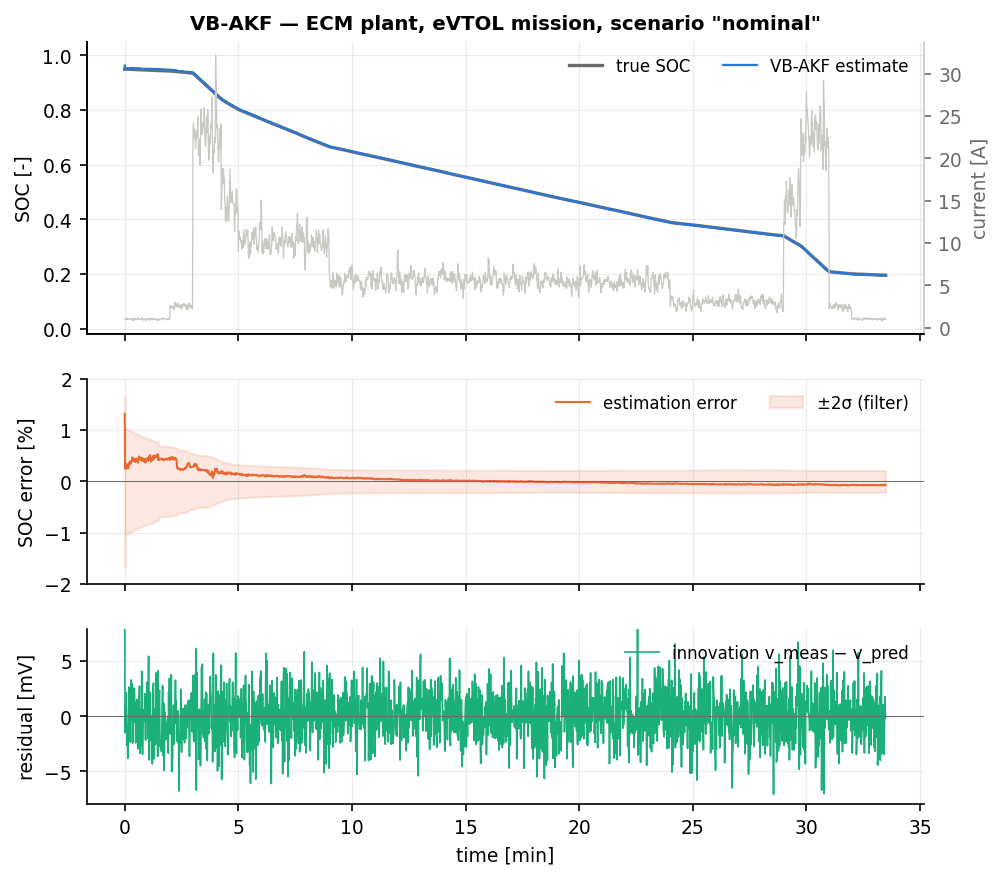
\includegraphics[width=\textwidth]{figures/cell_VBAKF_nominal.png}
\caption{VB-AKF on the nominal eVTOL mission: true and estimated SOC (top), estimation error with the $\pm 2\sigma$ band when available (middle), voltage residual (bottom).}
\end{figure}
\begin{figure}[H]\centering
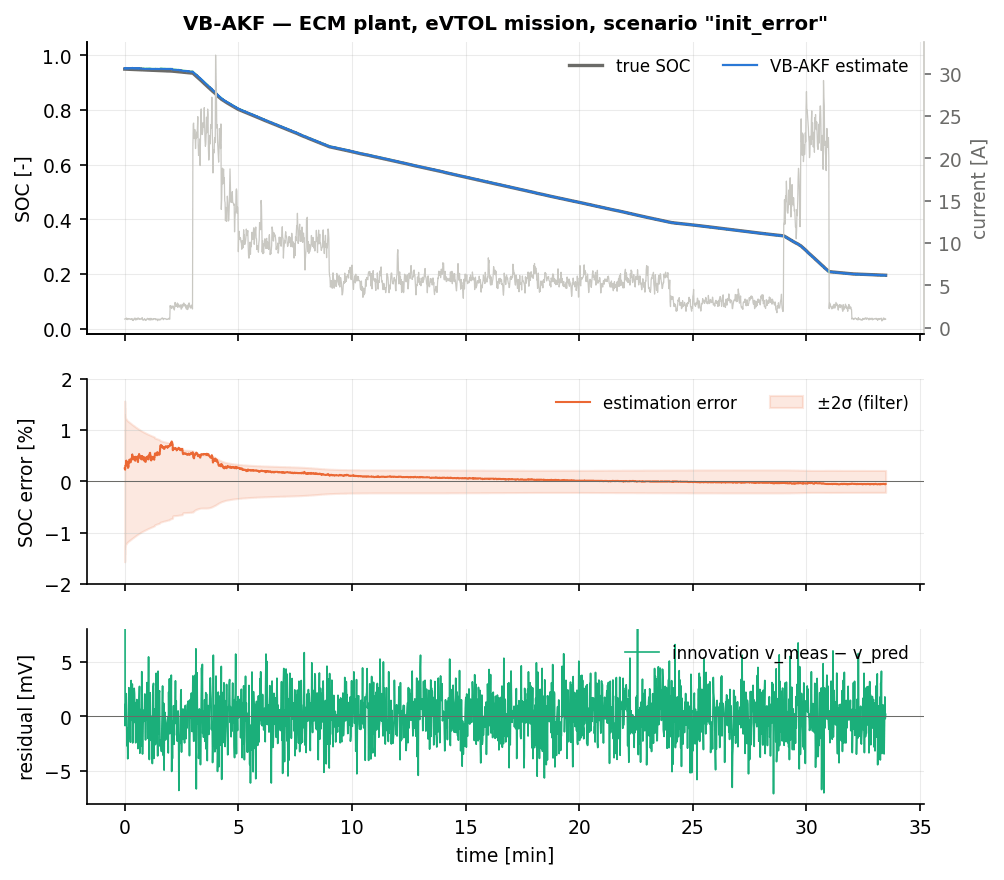
\includegraphics[width=\textwidth]{figures/cell_VBAKF_init_error.png}
\caption{VB-AKF with a 35\,\% initial SOC error.}
\end{figure}
\begin{figure}[H]\centering
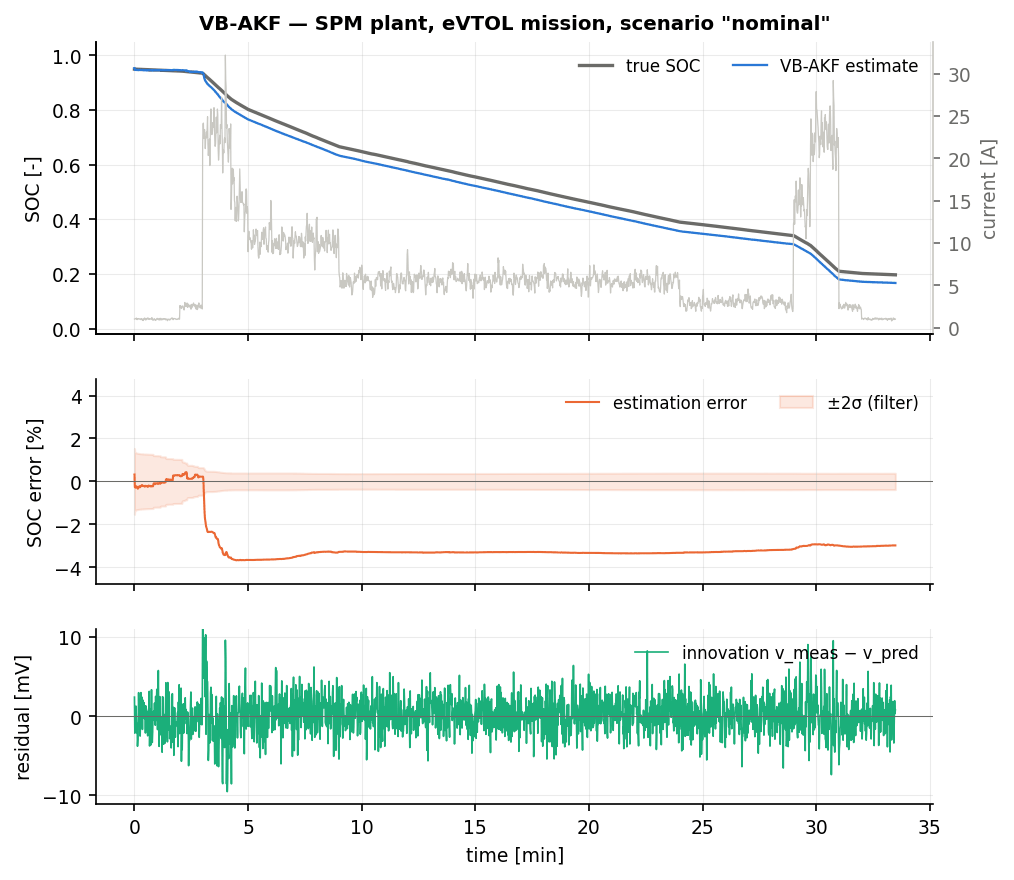
\includegraphics[width=\textwidth]{figures/cellspm_VBAKF_nominal.png}
\caption{VB-AKF on the electrochemical (single-particle) plant, nominal mission: the estimator uses a 2-RC ECM fitted to that plant and therefore sees a structured \SI{4}{\milli\volt} residual instead of white noise.}
\end{figure}

All figures below are three-seed means in \% SOC, as tabulated above; the plain \texttt{EKF} run on
the same data is the reference (\texttt{EKF ref.} column).  For orientation, the EKF scores
$\mathrm{rmse}_{ss}$ = 0.05\,\% on \texttt{nominal}, 0.12\,\% on \texttt{noise\_step}, 0.21\,\% on
\texttt{outliers}, 0.46\,\% on \texttt{sensor\_dropout}, 1.36\,\% on \texttt{param\_mismatch},
1.52\,\% on \texttt{aged\_cell} and 12.44\,\% on \texttt{combined} (where it never converges), and
3.73\,\% on the nominal SPM mission.

\paragraph{Benign scenarios.}  \texttt{nominal}: $\mathrm{rmse}=0.16\,\%$,
$\mathrm{rmse}_{ss}=0.05\,\%$, identical to the EKF's $0.15\,\%$ / $0.05\,\%$ in steady state --- as
it should be when the prior on $\sigma_v^2$ is already correct.  \texttt{init\_error}: converges at
$t=\SI{0}{\second}$, $\mathrm{rmse}=0.15\,\%$, $\mathrm{rmse}_{ss}=0.06\,\%$, maximum error
$0.63\,\%$ (EKF $0.14\,\%$ / $0.05\,\%$ / $0.62\,\%$).  The robustness mechanism costs one sample
here: the \SI{30}{\milli\volt} innovation caused by the initial SOC error is treated as an outlier
and partially down-weighted, so the first correction takes a few samples instead of one.  Both are
far inside the $2\,\%$ bound.

\paragraph{Target scenario \texttt{noise\_step}.}  On seed 1, $\hat\sigma_v$ averages
\SI{2.17}{\milli\volt} over $t\in[100,600)\,\si{\second}$ and \SI{19.99}{\milli\volt} over
$t\in[700,2010]\,\si{\second}$: the tenfold step is tracked to better than $0.1\,\%$.  The three-seed
SOC metrics show the benefit directly --- the EKF's steady-state error rises from $0.05\,\%$ on
\texttt{nominal} to $0.12\,\%$ here, while VB-AKF stays at $\mathbf{0.05\,\%}$, a $2.4\times$
reduction.  The mean normalised innovation squared is $0.989$ before and $0.996$ after the step,
against $1.099$ and $\mathbf{90.3}$ for the EKF, so the filter remains statistically consistent
throughout; $\mathrm{rmse}_v$ falls from \SI{2.89}{\milli\volt} to \SI{1.01}{\milli\volt}.

\paragraph{Target scenario \texttt{outliers}.}  This is where VB-AKF separates itself from the rest of
the family.  With 5\,\% of voltage samples corrupted by $\pm\SI{50}{\milli\volt}$ it reports
$\hat\sigma_v=\SI{11.4}{\milli\volt}$ --- the standard deviation of the contaminated distribution ---
and achieves $\mathrm{rmse}=\mathbf{0.12\,\%}$ and $\mathrm{rmse}_{ss}=\mathbf{0.05\,\%}$ against the
EKF's $0.52\,\%$ / $0.21\,\%$: a $4.3\times$ reduction of the full-run RMSE and $4.2\times$ in steady
state, with the maximum error down from $2.92\,\%$ to $1.60\,\%$ and immediate convergence against the
EKF's \SI{16}{\second}.  It is the best full-run result of the whole family on this scenario
(Fuzzy $0.25\,\%$, Sage--Husa $0.22\,\%$, IMM $0.18\,\%$, IAE $0.41\,\%$), and the reason is the
within-sample iteration of \eqref{eq:vb:beta}: an impulsive innovation inflates $\bm\Sigma$ for
\emph{that} sample and is therefore rejected, whereas the windowed estimators can only raise $\mR$
for the following $N$ samples, by which time the damage is done.

\paragraph{Model mismatch.}  \texttt{param\_mismatch}: $\mathrm{rmse}$ $1.28\to0.67\,\%$ and
$\mathrm{rmse}_{ss}$ $1.36\to0.79\,\%$ --- the second-best in the family after Sage--Husa.
\texttt{aged\_cell}: $1.18\to0.99\,\%$, $1.52\to1.27\,\%$.  \texttt{sensor\_dropout}:
$0.72\to0.17\,\%$, $0.46\to0.10\,\%$ ($4.2\times$ / $4.6\times$).  \texttt{combined}: the EKF never
converges ($t_\mathrm{conv}=$ --, $16.02\,\%$ / $12.44\,\%$); VB-AKF converges at
$t=\SI{1417}{\second}$ --- the earliest of the three covariance-matching filters --- with
$4.86\,\%$ / $\mathbf{1.87\,\%}$, i.e.\ $3.3\times$ / $6.7\times$ better, and the best steady-state
figure of the $\mR$-adapting group.  These numbers are within a few percent of the Sage--Husa and IAE
results, confirming that on \emph{persistent} disturbances all three covariance-matching mechanisms
converge to the same answer; the difference is confined to transients and impulses.  As for the other
adaptive filters the improvement in SOC is paid for in voltage prediction ($\mathrm{rmse}_v$
\SI{3.80}{\milli\volt}\,$\to$\,\SI{22.49}{\milli\volt} on \texttt{aged\_cell}).  \texttt{preisach}
is a draw ($0.58\,\%$ / $0.20\,\%$ for both filters, with immediate convergence against the EKF's
\SI{16}{\second}) and \texttt{cold} is slightly better than the EKF ($0.18\,\%$ against $0.16\,\%$ in
steady state but $0.23\,\%$ against $0.20\,\%$ over the full run).

\paragraph{Cost.}  \SI{872}{\nano\second}/step against \SI{478}{\nano\second}/step for the EKF and
\SI{500}{\nano\second}/step for IAE --- the most expensive of the three covariance-matching filters,
by about the factor $N_{vb}$ one expects.  The float32 build gives the same metrics to three digits
with no divergence on any of the twelve ECM scenarios.

\paragraph{Electrochemical (SPM) plant.}  With the estimator running a 2-RC ECM fitted to the
single-particle plant, the voltage residual is a structured, slowly varying \SI{4}{\milli\volt}
signal rather than white noise.  VB-AKF ends the nominal SPM mission at
$\mathrm{rmse}_{ss}=3.18\,\%$ against the EKF's $3.73\,\%$ --- a $15\,\%$ improvement, in the same
band as the other $\mR$-adapting filters (IAE $3.02\,\%$, Fuzzy $3.18\,\%$, Sage--Husa $3.33\,\%$)
and far behind the covariance-inflating ones (Fading-EKF $0.36\,\%$, STF $0.66\,\%$).  The
variational machinery behaves impeccably and that is precisely why it cannot help: the inverse-Gamma
posterior concentrates on $\beta/\alpha\approx(\SI{4}{\milli\volt})^2$, which is the \emph{correct}
description of the residual magnitude, and the Kalman update in \eqref{eq:vb:K} then correctly lowers
the gain.  But the conditional model behind \eqref{eq:vb:model} --- that everything not explained by
$h(\vx,\vu)$ is zero-mean white noise on the \emph{output} --- is false here; the discrepancy is a
deterministic function of the state and the current history.  Lowering the gain hands SOC to the
coulomb integrator, whose capacity and efficiency are the parts the ECM fit gets wrong, so the
estimate settles at a $3\,\%$ offset.  Trusting the measurement \emph{more}, which is what shortening
the filter memory does, is the correct response to structured model error, and is the mirror image of
the ECM \texttt{aged\_cell} case where the error lived in the output map and inflating $\mR$ was
right.  The one place where VB's per-sample reweighting still pays on this plant is
\texttt{param\_mismatch}, $3.13\to0.66\,\%$ --- a $4.7\times$ improvement and the best SPM
\texttt{param\_mismatch} result of any estimator in this family --- and \texttt{cold},
$7.35\to2.31\,\%$.  SPM \texttt{outliers} is the regression ($3.53\,\%$ against $1.99\,\%$): with the
gain already suppressed by the structured residual, additional impulse rejection only locks the
estimate harder onto the drifting integrator.

\section{Summary}
VB-AKF is the principled member of the covariance-matching family: it puts a conjugate prior on the
measurement variances, approximates the intractable joint posterior by the closest factorised one,
and obtains a fixed-point iteration that is positive by construction and needs no buffer.  Use it
when the measurement noise is both uncertain \emph{and} possibly heavy-tailed --- the within-sample
iteration gives it Student-$t$-like rejection of impulsive errors essentially for free, and on this
benchmark it is four times better than the EKF on an outlier-contaminated voltage channel while
tracking a tenfold noise step to $0.1\,\%$ and halving the SOC error it causes.  On the
electrochemical plant it gains only $15\,\%$ on the EKF, like every other $\mR$-adapting filter:
the inverse-Gamma posterior correctly identifies a \SI{4}{\milli\volt} residual, but the model behind
it --- white noise on the output --- is false, and lowering the gain is the wrong response.  Do not use it if the cost of $N_{vb}$ measurement
updates is unaffordable (use IAE or Sage--Husa, which cost one), if $\mR$ is genuinely non-diagonal,
or if you need to attribute the extra innovation energy to a specific cause.

% Copyright 2026 Sreeram Anil
% SPDX-License-Identifier: CC-BY-4.0
% =============================================================================
%  Fuzzy-logic adaptive Kalman filter (Mamdani covariance tuning)
% =============================================================================
\chapter{Fuzzy-logic adaptive Kalman filter (Fuzzy-AKF)}
\label{ch:fuzzyakf}

\section*{At a glance}
\begin{tabular}{@{}l>{\raggedright\arraybackslash}p{0.76\textwidth}@{}}
Family & Adaptive Kalman \\
Header & \texttt{include/estkit/filters/fuzzy\_akf.hpp} \\
Registered name & \texttt{Fuzzy-AKF} \\
State dimension & $n_x = 4$ (cell model) --- generic in $n_x, n_u, n_y$; window $N$ and grid $N_g$ are template parameters \\
Cost per step & EKF $+\,\mathcal{O}(n_y^2) + 3N_g$ flops; $\approx 730$\,ns/step, $N n_y$ reals of buffer, no heap \\
Primary references & \cite{loebis2004fuzzy,mamdani1975,zadeh1965,mohamed1999adaptive,jwo2007fuzzy} \\
\end{tabular}

\section{Motivation and aerospace/BMS relevance}
The covariance-matching estimators of \cref{ch:iaeakf} compute $\hat{\mR}$ in closed form and apply
it immediately.  That is statistically efficient but operationally brittle: the estimate inherits
the full variance of a short window, it can jump by an order of magnitude between consecutive
samples, and it has no notion of "how sure am I that something changed".  Engineers who have to
certify a filter frequently prefer a \emph{supervisor} that changes the tuning gradually, in a way
that can be stated in words and drawn on one page: "if the residuals are much larger than expected,
increase the assumed measurement noise a little; if they are much smaller, decrease it a little;
otherwise do nothing".

That is precisely a fuzzy inference system in the sense of Zadeh \cite{zadeh1965} and Mamdani
\cite{mamdani1975}.  Loebis, Sutton, Chudley and Naeem \cite{loebis2004fuzzy} applied it to the
navigation filter of an autonomous underwater vehicle: they form a scalar \emph{degree of matching}
(DoM) between the measured and the theoretical innovation covariance, feed it to a small rule base
with triangular membership functions, and use the defuzzified output to retune $\mR$ (and, in a
second loop, $\mQ$).  The same construction has since been combined with the strong tracking filter
for GPS navigation \cite{jwo2007fuzzy}.

The engineering value in a BMS is the rate limit.  A cell-voltage channel can be hit by a
\SI{50}{\milli\volt} spike from a single corrupted SPI frame; a closed-form estimator will respond
to the resulting window average with a step change in the gain, whereas a rate-limited fuzzy
supervisor slews the tuning smoothly and cannot be driven to an extreme by a short burst.  The price
is a slower response to a genuine change, and the whole design of this chapter is about where that
trade sits.

\section{Problem statement and assumptions}
The plant is \eqref{eq:sh:proc}--\eqref{eq:sh:meas}.  The filter carries a scalar
\emph{measurement-noise scaling} $s_k>0$ and uses
\begin{equation}
\hat{\mR}_k = s_k\,\mR(\xminus_k,\vu_k)
\label{eq:fz:R}
\end{equation}
in place of the nominal model covariance.  The design problem is to drive $s_k$ from the innovation
sequence.  We assume, as in \cref{ch:iaeakf}, that the innovations are approximately white
(\cref{as:iae:white}) and that the statistics are stationary over the window
(\cref{as:iae:stat}).

\section{Derivation}

\subsection{The degree of matching}
Let $\bm{e}_j=\vy_j-h(\xminus_j,\vu_j)$ and form the windowed sample covariance
\begin{equation}
\hat{\mC}_k = \frac{1}{N}\sum_{j=k-N+1}^{k}\bm{e}_j\bm{e}_j^\T
\label{eq:fz:C}
\end{equation}
and the filter's own prediction of it,
$\mS_k = \mH_k\Pminus_k\mH_k^\T + \hat{\mR}_{k-1}$.  Loebis et al.\ compare the two; the
dimensionless comparison used here is
\begin{equation}
\boxed{\;\mathrm{DoM}_k = \frac{\tr\hat{\mC}_k - \tr\mS_k}{\tr\mS_k}\;}
\label{eq:fz:dom}
\end{equation}
so that $\mathrm{DoM}_k=0$ means perfect matching, $\mathrm{DoM}_k>0$ means the filter is
over-confident (residuals larger than predicted) and $\mathrm{DoM}_k<0$ means it is
under-confident.  Normalising by $\tr\mS_k$ rather than using the raw difference makes the input
scale-free, so the same rule base and the same membership functions work for any measurement unit
and any operating point --- essential for a generic filter.

\subsection{The rule base}
Three membership functions partition the DoM universe.  With the normalised input
$d = \mathrm{DoM}_k/c$, where $c$ is the design constant \texttt{dom\_scale},
\begin{equation}
\mu_{\mathsf N}(d) = \begin{cases}1,& d\le-1\\ -d,& -1<d<0\\ 0,& d\ge0\end{cases}
\qquad
\mu_{\mathsf Z}(d) = \begin{cases}1-|d|,& |d|<1\\ 0,&\text{else}\end{cases}
\qquad
\mu_{\mathsf P}(d) = \begin{cases}0,& d\le0\\ d,& 0<d<1\\ 1,& d\ge1 .\end{cases}
\label{eq:fz:mf}
\end{equation}
The outer two are shoulders, so $\mu_{\mathsf N}+\mu_{\mathsf Z}+\mu_{\mathsf P}=1$ for every $d$
(a \emph{partition of unity}): at most two rules fire, the firing strengths are already normalised,
and the inference is continuous and piecewise linear in $d$.  The rule base is
\begin{center}
\begin{tabular}{@{}lll@{}}
\toprule
& antecedent & consequent \\
\midrule
$\mathsf{R}_1$ & IF $\mathrm{DoM}$ is $\mathsf N$ (negative) & THEN $\Delta$ is $\mathsf D$ (decrease $s$) \\
$\mathsf{R}_2$ & IF $\mathrm{DoM}$ is $\mathsf Z$ (zero)     & THEN $\Delta$ is $\mathsf H$ (hold $s$) \\
$\mathsf{R}_3$ & IF $\mathrm{DoM}$ is $\mathsf P$ (positive) & THEN $\Delta$ is $\mathsf I$ (increase $s$) \\
\bottomrule
\end{tabular}
\end{center}
with consequent membership functions that are unit-half-width triangles on the normalised output
axis $v\in[-1.5,1.5]$, centred at $c_1=-1$, $c_2=0$, $c_3=+1$:
$\mathrm{tri}_r(v)=\max(0,\,1-|v-c_r|)$.

\subsection{Mamdani inference and centroid defuzzification}
Mamdani's min-implication clips each consequent at its rule's firing strength
$w_r$, and max-aggregation takes the pointwise maximum:
\begin{equation}
\mu^{\text{agg}}(v) = \max_{r\in\{1,2,3\}}\ \min\!\big(w_r,\ \mathrm{tri}_r(v)\big),
\qquad w_1=\mu_{\mathsf N}(d),\ w_2=\mu_{\mathsf Z}(d),\ w_3=\mu_{\mathsf P}(d).
\label{eq:fz:agg}
\end{equation}
The crisp output is the centre of area of the aggregated set,
\begin{equation}
v^\star = \frac{\int v\,\mu^{\text{agg}}(v)\,\mathrm{d}v}{\int \mu^{\text{agg}}(v)\,\mathrm{d}v}
\;\approx\; \frac{\sum_{g=1}^{N_g} v_g\,\mu^{\text{agg}}(v_g)}{\sum_{g=1}^{N_g}\mu^{\text{agg}}(v_g)},
\qquad v_g = -1.5 + 3\frac{g-1}{N_g-1},
\label{eq:fz:centroid}
\end{equation}
evaluated on a fixed grid of $N_g$ points.  The grid is what makes this a genuine Mamdani centroid
rather than the weighted-average (Sugeno) short cut; it costs $3N_g$ multiply--adds per sample,
$123$ for the default $N_g=41$, which is small next to the EKF's $\approx500$ flops.

\subsection{The tuning law and its fixed point}
The defuzzified output is interpreted as an increment of $\ln s$:
\begin{equation}
s_k = \mathrm{clamp}\Big(s_{k-1}\exp\big(\delta\, v^\star\big),\ s_{\min},\ s_{\max}\Big),
\label{eq:fz:law}
\end{equation}
where $\delta = \texttt{opts.step}$ is the maximum change of $\ln s$ per sample, i.e.\ a
\emph{rate limit}.  Working in the logarithm makes the law scale-invariant (a factor-of-ten error is
corrected in the same number of samples whether $s$ is $1$ or $100$) and guarantees $s_k>0$.

The fixed point of \eqref{eq:fz:law} is $v^\star=0$, which by \eqref{eq:fz:mf} requires
$\mathrm{DoM}_k=0$, i.e.\ $\tr\mS_k=\tr\hat{\mC}_k$; writing this out,
\begin{equation}
s^\star\,\tr\mR = \tr\hat{\mC}_k - \tr\big(\mH_k\Pminus_k\mH_k^\T\big),
\label{eq:fz:fp}
\end{equation}
which is \emph{exactly} the IAE estimator \eqref{eq:iae:R} in trace form.  The fuzzy supervisor is
therefore a rate-limited, smoothed realisation of innovation-based adaptive estimation: it converges
to the same answer, but it slews there at no more than $\delta$ nepers per sample and it cannot be
displaced from it by a short burst of large innovations.  Stating the fixed point explicitly is what
turns a heuristic into an analysable controller --- and it immediately gives the design rule for
$\delta$: the time to correct a factor-$\kappa$ error in $s$ is $\ln\kappa/\delta$ samples.

\section{Algorithm}
\begin{algorithm}[H]
\caption{Fuzzy-AKF --- one sampling period}
\begin{algorithmic}[1]
\Require $\xplus_{k-1},\Pplus_{k-1},\vu_{k-1},\vy_k,\vu_k,s_{k-1}$, ring buffer and running sum $\Sigma$
\State \textbf{Time update:} $\xminus_k\gets f(\xplus_{k-1},\vu_{k-1})$;\quad $\Pminus_k\gets\mF\Pplus_{k-1}\mF^\T+\mQ_k$
\State \textbf{Innovation:} $\mH\gets\partial h/\partial\vx|_{\xminus_k}$;\quad $\bm{e}_k\gets\vy_k-h(\xminus_k,\vu_k)$
\State \textbf{Window:} slide the ring buffer, $\Sigma\gets\Sigma-\bm{e}_{k-N}\bm{e}_{k-N}^\T+\bm{e}_k\bm{e}_k^\T$;\quad $\hat{\mC}_k\gets\Sigma/n$
\If{$n\ge N_{\min}$}
  \State $\mS\gets\mH\Pminus_k\mH^\T+s_{k-1}\mR_k$;\quad $\mathrm{DoM}\gets(\tr\hat{\mC}_k-\tr\mS)/\tr\mS$
  \State $d\gets\mathrm{clamp}(\mathrm{DoM}/c,-2,2)$;\quad evaluate $w_{1,2,3}$ from \eqref{eq:fz:mf}
  \State $v^\star\gets$ centroid of $\max_r\min(w_r,\mathrm{tri}_r(\cdot))$ on the $N_g$-point grid
  \State $s_k\gets\mathrm{clamp}(s_{k-1}e^{\delta v^\star},s_{\min},s_{\max})$
\EndIf
\State $\hat{\mR}_k\gets s_k\mR_k$
\State \textbf{Gain and update:} $\mS_k\gets\mH\Pminus_k\mH^\T+\hat{\mR}_k$;\quad $\mK_k\gets\Pminus_k\mH^\T\mS_k\inv$;\quad
       $\xplus_k\gets\xminus_k+\mK_k\bm{e}_k$;\quad Joseph update of $\Pplus_k$
\State \textbf{Constrain:} $\xplus_k\gets\mathrm{constrain}(\xplus_k)$
\Ensure $\xplus_k,\Pplus_k,s_k$
\end{algorithmic}
\end{algorithm}

\section{Application to the battery model}
With $n_y=1$ the traces in \eqref{eq:fz:dom} are scalars and
$\mathrm{DoM}_k = (\hat C_k - S_k)/S_k$ with $\hat C_k$ the mean squared voltage innovation over the
window.  Options used in the benchmark: $N=50$ samples ($=\SI{5}{\second}$, the window length used
by Loebis et al.\ scaled to this sample rate), $N_g=41$ grid points, $c=0.5$ (a $50\,\%$ covariance
mismatch saturates the "negative"/"positive" membership), $\delta=0.3$, $s\in[0.2,\,2\times10^3]$.

The rate limit deserves a word.  $\delta=0.3$ per sample is $\SI{3}{\per\second}$ at
\SI{10}{\hertz}, so $s$ can change by a factor of $e^3\approx20$ per second and needs
$\ln(93)/0.3\approx15$ samples $=\SI{1.5}{\second}$ to cover the factor-$93$ change demanded by the
\texttt{noise\_step} scenario --- fast enough to be useful, slow enough that a single corrupted
sample (which moves the window mean by $1/N$ of its value) barely moves $s$.  Values
$\delta\in\{0.002,0.01,0.05,0.1,0.3\}$ were evaluated; below $\delta\approx0.1$ the supervisor is too
slow to correct the large mismatch of the \texttt{combined} scenario within the mission and the
filter never reaches the $2\,\%$ band, which is why the comparatively brisk $0.3$ was adopted.  The
saturation constant $c=0.5$ and the bounds were not found to be critical (the metrics change by
under $10\,\%$ over $c\in[0.2,2]$).

\section{Implementation notes}
\begin{itemize}[leftmargin=1.4em]
\item \textbf{Heap-free fuzzy engine.}  The membership functions are evaluated in closed form, the
      aggregation and centroid are computed on a compile-time-sized grid
      (\texttt{template<class Model,int NWIN,int NG>}), and the only transcendental call is a single
      guarded \texttt{exp} per sample.  No lookup tables, no dynamic memory, fully deterministic
      execution time --- the properties that make a fuzzy supervisor attractive on a safety-related
      MCU in the first place.
\item \textbf{Partition of unity.}  Because $\sum_r w_r = 1$ by construction, no normalisation of
      the firing strengths is needed and the denominator of \eqref{eq:fz:centroid} can never vanish
      (it is guarded anyway).
\item \textbf{Buffer.}  $N n_y$ reals ($400$\,bytes for the cell model) plus one running sum,
      updated in $\mathcal{O}(n_y^2)$.
\item \textbf{Cost.}  \SI{727}{\nano\second}/step against \SI{478}{\nano\second}/step for the EKF.
      The overhead is dominated by the $3N_g=123$ grid evaluations; dropping to $N_g=11$ or using
      Sugeno singletons would remove most of it at the cost of a slightly coarser centroid.
\item \textbf{float32.}  Metrics agree with the double build to three digits; no divergence.
\item \textbf{Limitations.}  Being a rate-limited IAE, it inherits IAE's inability to distinguish
      sensor noise from model error, and it adds a lag.  It also adapts only $\mR$; Loebis et al.\
      use a second fuzzy loop for $\mQ$, which is not implemented here for the identifiability
      reasons set out in \cref{ch:sagehusaakf}.
\end{itemize}

\section{Benchmark results}
% Copyright 2026 Sreeram Anil
% SPDX-License-Identifier: CC-BY-4.0
\begin{table}[H]\centering\footnotesize\setlength{\tabcolsep}{4pt}
\caption{Fuzzy-AKF: cell-level benchmark on the eVTOL mission (mean over seeds; RMSE and max error in \% SOC; $t_\mathrm{conv}$: first time the error stays below 2\,\% for 60\,s, -- = never; EKF reference: steady-state RMSE of the plain EKF on the same data).}\label{tab:cell_FuzzyAKF}
\begin{tabular}{llrrrrrcrr}\toprule
plant & scenario & RMSE & RMSE$_\mathrm{ss}$ & max & $t_\mathrm{conv}$ [s] & RMSE$_v$ [mV] & div. & EKF ref. & ns/step \\ \midrule
ECM & nominal & 0.19 & 0.05 & 1.15 & 0 & 0.79 & no & 0.05 & 727 \\
ECM & init\_error & 0.16 & 0.08 & 0.71 & 0 & 2.12 & no & 0.05 & 729 \\
ECM & current\_bias & 0.54 & 0.64 & 1.39 & 0 & 0.87 & no & 0.61 & 728 \\
ECM & noise\_step & 0.19 & 0.05 & 1.15 & 0 & 1.02 & no & 0.12 & 728 \\
ECM & outliers & 0.25 & 0.05 & 2.50 & 0 & 1.47 & no & 0.21 & 726 \\
ECM & cold & 0.20 & 0.20 & 1.17 & 0 & 1.89 & no & 0.16 & 725 \\
ECM & hot & 0.18 & 0.03 & 1.00 & 0 & 0.54 & no & 0.03 & 727 \\
ECM & aged\_cell & 1.04 & 1.25 & 2.62 & 0 & 22.45 & no & 1.52 & 725 \\
ECM & param\_mismatch & 0.83 & 0.96 & 1.91 & 0 & 6.12 & no & 1.36 & 723 \\
ECM & sensor\_dropout & 0.19 & 0.06 & 1.15 & 0 & 0.88 & no & 0.46 & 723 \\
ECM & preisach & 0.61 & 0.20 & 1.80 & 0 & 0.82 & no & 0.20 & 728 \\
ECM & combined & 5.67 & 2.56 & 14.93 & 1753 & 15.01 & no & 12.44 & 735 \\
\midrule
SPM & nominal & 3.11 & 3.18 & 3.80 & 0 & 1.53 & no & 3.73 & 698 \\
SPM & init\_error & 3.42 & 3.43 & 4.29 & 0 & 2.45 & no & 3.81 & 701 \\
SPM & current\_bias & 4.45 & 5.16 & 5.85 & 0 & 1.90 & no & 5.69 & 698 \\
SPM & noise\_step & 3.12 & 3.20 & 3.80 & 0 & 2.38 & no & 3.30 & 708 \\
SPM & outliers & 2.72 & 2.70 & 4.09 & 0 & 2.56 & no & 1.99 & 697 \\
SPM & cold & 3.26 & 3.09 & 4.52 & 0 & 16.11 & no & 7.35 & 692 \\
SPM & hot & 2.09 & 2.14 & 2.52 & 0 & 0.78 & no & 2.16 & 700 \\
SPM & param\_mismatch & 1.77 & 1.99 & 2.43 & 0 & 3.94 & no & 3.13 & 688 \\
SPM & sensor\_dropout & 3.30 & 3.36 & 4.13 & 0 & 2.01 & no & 5.31 & 700 \\
\bottomrule\end{tabular}\end{table}

\begin{figure}[H]\centering
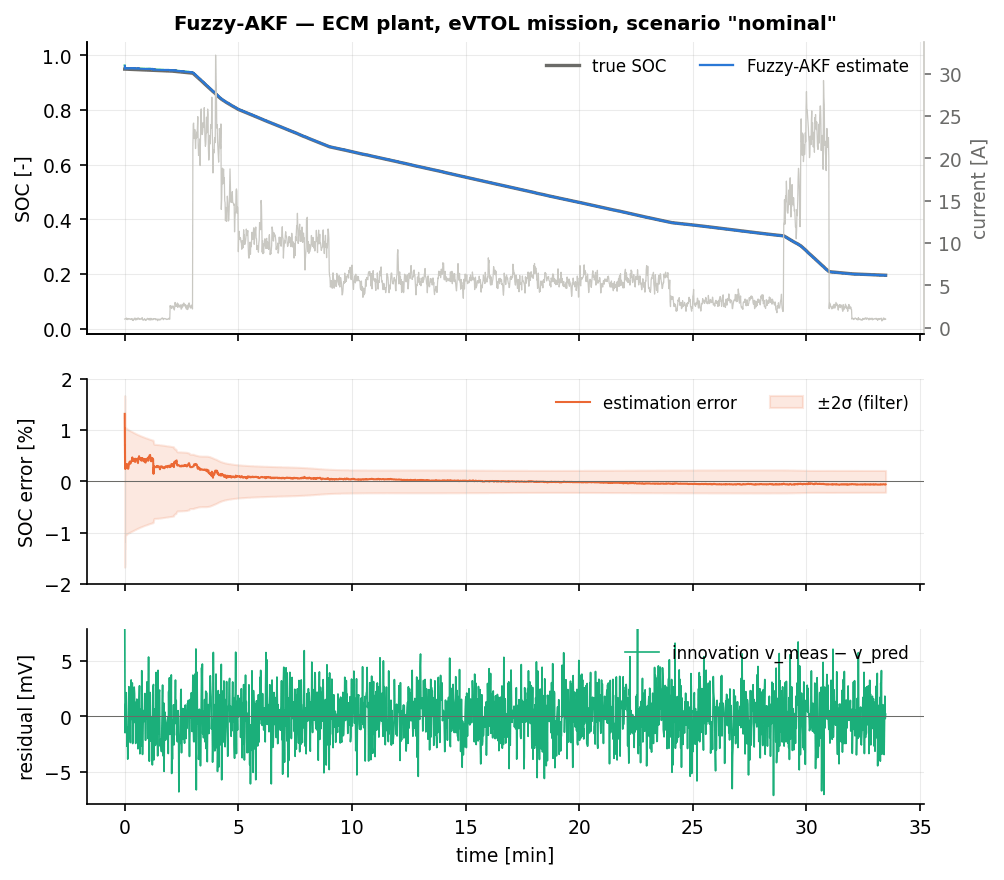
\includegraphics[width=\textwidth]{figures/cell_FuzzyAKF_nominal.png}
\caption{Fuzzy-AKF on the nominal eVTOL mission: true and estimated SOC (top), estimation error with the $\pm 2\sigma$ band when available (middle), voltage residual (bottom).}
\end{figure}
\begin{figure}[H]\centering
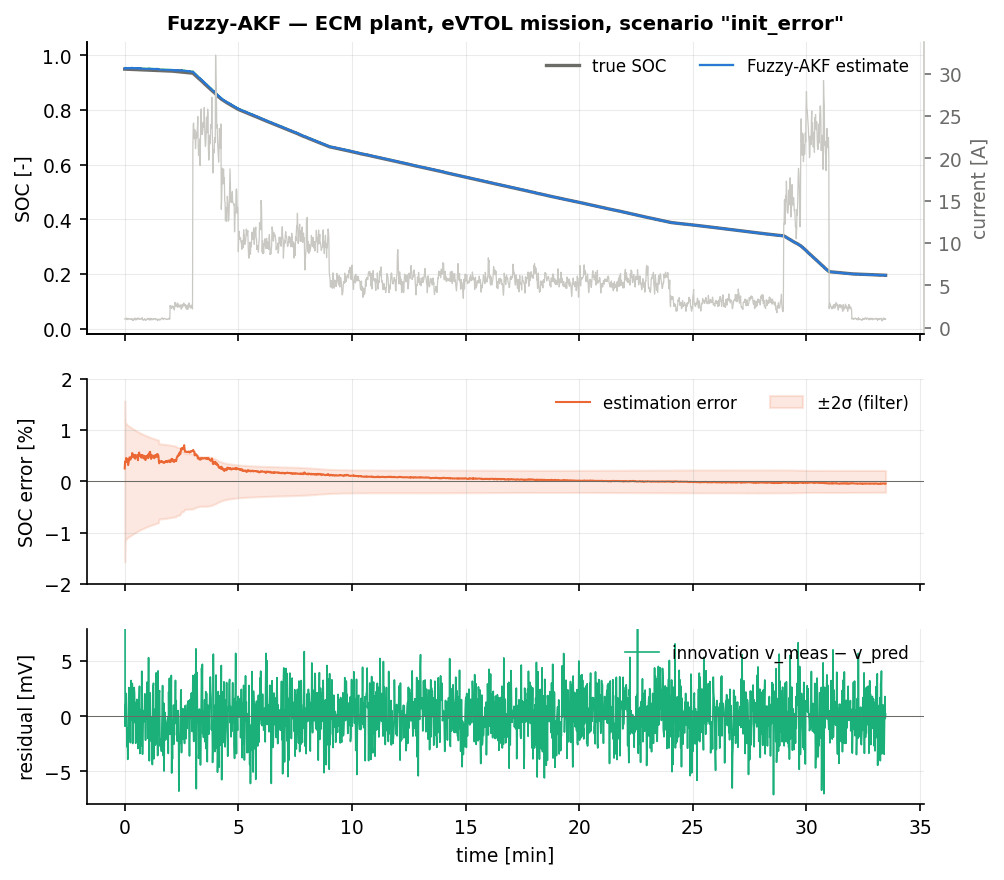
\includegraphics[width=\textwidth]{figures/cell_FuzzyAKF_init_error.png}
\caption{Fuzzy-AKF with a 35\,\% initial SOC error.}
\end{figure}
\begin{figure}[H]\centering
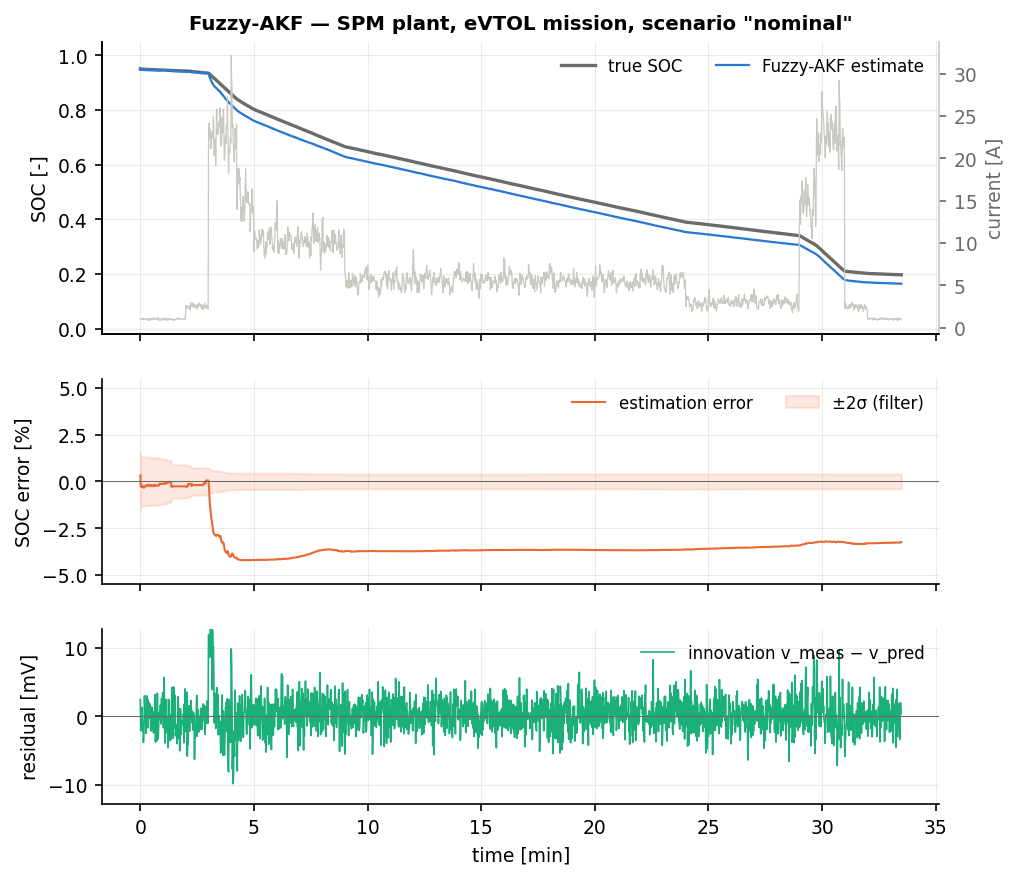
\includegraphics[width=\textwidth]{figures/cellspm_FuzzyAKF_nominal.png}
\caption{Fuzzy-AKF on the electrochemical (single-particle) plant, nominal mission: the estimator uses a 2-RC ECM fitted to that plant and therefore sees a structured \SI{4}{\milli\volt} residual instead of white noise.}
\end{figure}

All figures below are three-seed means in \% SOC, as tabulated above; the plain \texttt{EKF} run on
the same data is the reference (\texttt{EKF ref.} column).  For orientation, the EKF scores
$\mathrm{rmse}_{ss}$ = 0.05\,\% on \texttt{nominal}, 0.12\,\% on \texttt{noise\_step}, 0.21\,\% on
\texttt{outliers}, 0.46\,\% on \texttt{sensor\_dropout}, 1.36\,\% on \texttt{param\_mismatch},
1.52\,\% on \texttt{aged\_cell} and 12.44\,\% on \texttt{combined} (where it never converges), and
3.73\,\% on the nominal SPM mission.

\paragraph{Benign scenarios.}  \texttt{nominal}: $\mathrm{rmse}=0.19\,\%$,
$\mathrm{rmse}_{ss}=0.05\,\%$ against the EKF's $0.15\,\%$ / $0.05\,\%$; the supervisor settles at
$s\approx1.10$, i.e.\ it detects (correctly) that the true innovation energy is about $10\,\%$ above
the nominal model value, mostly because of the ADC quantisation the model does not represent.
\texttt{init\_error}: $0.16\,\%$ / $0.08\,\%$, converging at $t=\SI{0}{\second}$ with a maximum error
of $0.71\,\%$.  Both well inside the $2\,\%$ bound.

\paragraph{Target scenario \texttt{noise\_step}.}  Averaged over $t\in[100,600)\,\si{\second}$ on
seed 1 the scaling is $s=1.10$; over $t\in[700,2010]\,\si{\second}$ it is $s=93.3$, i.e.\
$\hat\sigma_v=\sqrt{93.3}\times\SI{2.09}{\milli\volt}=\SI{20.2}{\milli\volt}$ against the true
\SI{20}{\milli\volt} --- a $1\,\%$ error in the identified standard deviation.  The three-seed SOC
metrics confirm that this is worth having: the EKF's steady-state error rises from $0.05\,\%$ on
\texttt{nominal} to $0.12\,\%$ here, while Fuzzy-AKF holds $\mathbf{0.05\,\%}$, a $2.4\times$
reduction.  The mean normalised innovation squared is $1.019$ before and $1.020$ after the step,
versus $1.099$ and $\mathbf{90.3}$ for the EKF: consistency is fully restored.  The
voltage-prediction error falls from \SI{2.89}{\milli\volt} to \SI{1.02}{\milli\volt}.

\paragraph{Target scenario \texttt{outliers}.}  With $5\,\%$ of samples corrupted by
$\pm\SI{50}{\milli\volt}$ the supervisor settles at $s=31.0$
($\hat\sigma_v=\SI{11.6}{\milli\volt}$, the standard deviation of the contaminated distribution) and
gives $\mathrm{rmse}=0.25\,\%$, $\mathrm{rmse}_{ss}=\mathbf{0.05\,\%}$ against the EKF's $0.52\,\%$ /
$0.21\,\%$ --- a $2.1\times$ reduction of the full-run RMSE and $4.2\times$ in steady state, tying
the variational filter of \cref{ch:vbakf} on the steady-state metric (though VB is twice as good over
the full run, $0.12\,\%$, because it rejects each spike as it arrives).  The rate limit is both the
strength and the weakness here: it prevents the supervisor from being yanked around by the spikes ---
the mean NIS of $2.03$ shows that the filter deliberately does \emph{not} inflate $\mR$ enough to
absorb the outliers into its consistency statistic --- but it also means each individual outlier is
processed with a gain that is only moderately reduced, and the maximum error stays at $2.50\,\%$
against VB's $1.60\,\%$.

\paragraph{Model mismatch.}  \texttt{param\_mismatch}: $\mathrm{rmse}$ $1.28\to0.83\,\%$ and
$\mathrm{rmse}_{ss}$ $1.36\to0.96\,\%$.  \texttt{sensor\_dropout}: $0.72\to0.19\,\%$,
$0.46\to0.06\,\%$ ($3.8\times$ / $7.7\times$, second only to IAE).  \texttt{aged\_cell}:
$1.18\to1.04\,\%$, $1.52\to1.25\,\%$.  \texttt{combined}: the EKF never converges
($t_\mathrm{conv}=$ --, $16.02\,\%$ / $12.44\,\%$); Fuzzy-AKF converges at $t=\SI{1753}{\second}$
with $5.67\,\%$ / $2.56\,\%$, a $2.8\times$ / $4.9\times$ improvement but the slowest convergence and
the weakest steady-state figure of the four $\mR$-adapting filters --- which is the rate limit showing
up exactly where the theory says it will, since the scenario demands a factor-of-sixty change in $s$
from the first sample onwards.  \texttt{preisach} (Preisach hysteresis with the corrected sign
convention in the truth plant) is a draw with the EKF in steady state ($0.20\,\%$ for both, full-run
$0.61\,\%$ against $0.58\,\%$) but converges immediately against the EKF's \SI{16}{\second};
\texttt{cold} ($0.20\,\%$ against $0.16\,\%$) and \texttt{current\_bias} ($0.64\,\%$ against
$0.61\,\%$) are marginally worse, the latter necessarily so, since an input-side error does not show
up in the innovation covariance.

\paragraph{Cost.}  \SI{727}{\nano\second}/step against the EKF's \SI{478}{\nano\second}/step, behind
only VB-AKF and the two multiple-model estimators; the Mamdani centroid grid is $\approx40\,\%$ of the
overhead.

\paragraph{Electrochemical (SPM) plant.}  On the single-particle plant the 2-RC ECM leaves a
structured, slowly varying \SI{4}{\milli\volt} residual, and the fuzzy supervisor reads it exactly as
its rule base instructs: $\tr\hat{\mC}_k$ exceeds $\tr\mS_k$, $\mathrm{DoM}_k$ is firmly positive,
rule $\mathsf{R}_3$ fires at full strength, and $s$ ramps up until the two match.  The result is
$\mathrm{rmse}_{ss}=3.18\,\%$ on the nominal SPM mission against the EKF's $3.73\,\%$, a $15\,\%$
improvement --- essentially identical to the other $\mR$-adapting filters (IAE $3.02\,\%$, VB
$3.18\,\%$, Sage--Husa $3.33\,\%$) and an order of magnitude behind the covariance-inflating ones
(Fading-EKF $0.36\,\%$, STF $0.66\,\%$).  The fixed-point identity \eqref{eq:fz:fp} explains why the
whole $\mR$-adapting group lands in the same place: they all converge to the same covariance-matching
solution, and that solution is the wrong one here.  Matching the innovation covariance means
declaring the voltage channel noisy and reducing the gain, which hands SOC to the coulomb integrator
--- and on the SPM plant the integrator is the faulty part, because the fitted capacity and coulombic
efficiency do not reproduce the true lithium inventory.  The measurement is the trustworthy part: the
ECM's $\ocv(\soc)$ map was fitted to this plant.  Under structured model error the correct move is to
shorten the filter's memory so recent measurements outweigh the accumulated model --- inflating $\mP$
--- and covariance matching does the exact opposite.  Where the SPM scenario adds a second error on
top, the supervisor earns its keep: \texttt{cold} $7.35\to3.09\,\%$ ($2.4\times$),
\texttt{param\_mismatch} $3.13\to1.99\,\%$, \texttt{sensor\_dropout} $5.31\to3.36\,\%$ and
\texttt{current\_bias} $5.69\to5.16\,\%$.  SPM \texttt{outliers} ($2.70\,\%$ against $1.99\,\%$) is
the only regression, and it is the mildest of the four $\mR$-adapting filters --- the rate limit that
costs convergence speed on \texttt{combined} is what protects it here.

\section{Summary}
A three-rule Mamdani supervisor driven by the normalised covariance mismatch is a rate-limited
implementation of innovation-based adaptive estimation, with the same fixed point and a slew rate
the designer chooses explicitly.  Use it when the tuning must change smoothly and explainably --- it
identifies a tenfold voltage-noise step to within $1\,\%$, restores $\overline{\mathrm{NIS}}\approx1$
where the EKF reaches $90$, cuts the steady-state error on \texttt{param\_mismatch}
by $1.4\times$, on \texttt{sensor\_dropout} by $7.7\times$ and on \texttt{outliers} by $4.2\times$.  Do not use it where a fast per-sample reaction is required: on
impulsive noise the variational filter of \cref{ch:vbakf} is twice as good over the full run, and on a large,
sudden model mismatch the rate limit costs several hundred seconds of convergence time.  Its real
attraction is not accuracy but transparency: every element of the mapping from residual to tuning
can be written on one slide and defended to a certification authority.  Like every filter built on
the covariance-matching fixed point \eqref{eq:fz:fp}, it cannot help when the residual is structured
model error: on the electrochemical plant it gains $15\,\%$ on the EKF where a fading-memory filter
gains a factor of ten.

% Copyright 2026 Sreeram Anil
% SPDX-License-Identifier: CC-BY-4.0
% =============================================================================
%  Strong tracking filter (suboptimal fading factor)
% =============================================================================
\chapter{Strong tracking filter (STF)}
\label{ch:stf}

\section*{At a glance}
\begin{tabular}{@{}l>{\raggedright\arraybackslash}p{0.76\textwidth}@{}}
Family & Adaptive Kalman \\
Header & \texttt{include/estkit/filters/stf.hpp} \\
Registered name & \texttt{STF} \\
State dimension & $n_x = 4$ (cell model) --- generic in $n_x, n_u, n_y$ \\
Cost per step & EKF $+$ one $n_x\times n_x$ scale-and-add $+\,\mathcal{O}(n_y^2 n_x)$; $\approx 530$\,ns/step, no heap \\
Primary references & \cite{zhoufrank1996stf,xia1994adaptive,jwo2007fuzzy,simon2006,jazwinski1970} \\
\end{tabular}

\section{Motivation and aerospace/BMS relevance}
A converged Kalman filter is a very confident object.  After a few hundred samples $\Pplus$ has
settled at its steady-state value, the gain is small, and the filter's estimate is dominated by its
own model.  That is exactly what one wants when the model is right --- and exactly what one does not
want when it is not.  A sudden manoeuvre, a change of the vehicle's mass, a cell whose internal
resistance has grown by $25\,\%$ since the model was identified: in every case the innovation
sequence stops being white and starts carrying a systematic component that the filter, having
already decided that it knows the state, largely ignores.  Anderson and Moore
\cite[Sec.~4.4]{andersonmoore1979} call the resulting slow, monotone error growth \emph{divergence
through model mismatch}; it is the single most common failure mode of Kalman filters in the field.

Zhou and Frank \cite{zhoufrank1996stf} proposed a direct cure.  They keep the minimum-variance
requirement of the Kalman filter but \emph{add} a second requirement: the innovation sequence must
be orthogonal at all non-zero lags, that is, white.  Whiteness of the innovations is the classical
signature of an optimal filter (Kailath's innovations representation, \cite[Ch.~9]{kailath2000});
if the residuals are still correlated, information remains in them that the filter has failed to
extract.  Zhou and Frank enforce the second requirement, suboptimally, by inserting a single scalar
\emph{fading factor} $\lambda_k\ge 1$ in front of the propagated part of the prediction covariance.
The effect is that the filter's memory is shortened automatically and only when the innovations say
it must be, which is why the method is called \emph{strong tracking}: it tracks abrupt changes
strongly while degenerating to the ordinary EKF when nothing is wrong.

The STF is widely used in fault detection and isolation, in manoeuvring-target tracking, and in
GNSS/INS integration where it is often combined with a fuzzy supervisor \cite{jwo2007fuzzy}.  The
closely related "adaptive fading Kalman filter" of Xia et al.\ \cite{xia1994adaptive} uses the same
inflation with a differently computed factor.  In a BMS the natural targets are an aged cell whose
parameters no longer match the stored map, a current-sensor bias, and the transient after a reset
with a bad initial SOC.

\section{Problem statement and assumptions}
The plant is \eqref{eq:sh:proc}--\eqref{eq:sh:meas}.  Define the innovation
$\bm{e}_k=\vy_k-h(\xminus_k,\vu_k)$.  The STF seeks a gain sequence $\{\mK_k\}$ such that
\begin{align}
&\text{(i)}\quad \E{(\vx_k-\xplus_k)(\vx_k-\xplus_k)^\T} \ \text{is minimised}, \label{eq:stf:r1}\\
&\text{(ii)}\quad \E{\bm{e}_{k+j}\,\bm{e}_{k}^\T} = \bm 0, \qquad j = 1,2,\dots \label{eq:stf:r2}
\end{align}
\begin{assumption}\label{as:stf:mismatch}
The model error can be represented, to first order, by an unknown multiplicative inflation of the
propagated prediction covariance, $\Pminus_k=\lambda_k\mF_{k-1}\Pplus_{k-1}\mF_{k-1}^\T+\mQ_{k-1}$
with an unknown scalar $\lambda_k\ge1$.
\end{assumption}
\begin{assumption}\label{as:stf:stat}
The actual innovation covariance can be estimated recursively from the innovation sequence itself
with a forgetting factor $\rho\in(0,1]$.
\end{assumption}

\section{Derivation}

\subsection{Why orthogonality gives the fading factor}
For an optimal filter, the innovation is the part of $\vy_k$ that is not predictable from
$\vy_{1:k-1}$, hence orthogonal to everything already used.  Suppose the filter is \emph{not}
optimal because the model is wrong.  Write the true prediction error as
$\tilde{\vx}^-_k = \vx_k - \xminus_k$, so that $\bm{e}_k = \mH_k\tilde{\vx}^-_k+\vv_k$ to first order.
Propagating one step through the (correct) dynamics and the (incorrect) filter gives
\begin{equation}
\tilde{\vx}^-_{k+1} = \big(\mF_k - \mF_k\mK_k\mH_k\big)\tilde{\vx}^-_k + \vw_k - \mF_k\mK_k\vv_k ,
\label{eq:stf:errprop}
\end{equation}
and therefore, using $\E{\vw_k\bm{e}_k^\T}=\bm 0$ and $\E{\vv_k\bm{e}_k^\T}=\mR_k$,
\begin{equation}
\E{\bm{e}_{k+1}\bm{e}_k^\T} = \mH_{k+1}\mF_k\Big[\E{\tilde{\vx}^-_k\bm{e}_k^\T} - \mK_k\,\E{\bm{e}_k\bm{e}_k^\T}\Big].
\label{eq:stf:lag1}
\end{equation}
Requirement \eqref{eq:stf:r2} at $j=1$ is met for all $\mH_{k+1}\mF_k$ if the bracket vanishes,
i.e.\ if
\begin{equation}
\mK_k = \E{\tilde{\vx}^-_k\bm{e}_k^\T}\Big(\E{\bm{e}_k\bm{e}_k^\T}\Big)\inv .
\label{eq:stf:Kopt}
\end{equation}
This is precisely the Kalman gain \emph{provided} the two expectations are the true ones.  The
filter computes them from its own covariance as $\Pminus_k\mH_k^\T$ and
$\mH_k\Pminus_k\mH_k^\T+\mR_k$; if the model is wrong, its $\Pminus_k$ is too small, the gain is
too small, and \eqref{eq:stf:lag1} does not vanish.  The remedy is to enlarge $\Pminus_k$ until the
filter's predicted innovation covariance equals the \emph{measured} one, because then
\eqref{eq:stf:Kopt} is satisfied with the correct second moments and all higher lags follow by
induction on \eqref{eq:stf:errprop}.  The condition is
\begin{equation}
\boxed{\;\bm{V}_k \;\triangleq\; \E{\bm{e}_k\bm{e}_k^\T} \;=\; \mH_k\Pminus_k\mH_k^\T + \mR_k\;}
\label{eq:stf:cond}
\end{equation}
which is the same covariance-matching identity that drives the filters of
\cref{ch:sagehusaakf} and \cref{ch:iaeakf} --- but here it is solved for a covariance inflation rather than for
$\mR$.  This is the fundamental ambiguity of the whole family, and it is discussed again below.

\subsection{Solving for $\lambda_k$}
Insert \cref{as:stf:mismatch} into \eqref{eq:stf:cond}:
\begin{equation}
\bm{V}_k = \lambda_k\,\mH_k\mF_{k-1}\Pplus_{k-1}\mF_{k-1}^\T\mH_k^\T + \mH_k\mQ_{k-1}\mH_k^\T + \mR_k .
\label{eq:stf:sub}
\end{equation}
For $n_y>1$ this is an over-determined system in the single scalar $\lambda_k$; Zhou and Frank take
the trace of both sides, which is the least-squares solution in the Frobenius sense when the two
sides are constrained to differ by a multiple of the identity.  Introducing the softening factor
$\beta\ge 1$, which replaces $\mR_k$ by $\beta\mR_k$ and so makes the filter reluctant to declare a
mismatch, one obtains
\begin{equation}
\lambda_k = \max\!\left(1,\; \frac{\tr\bm{N}_k}{\tr\bm{M}_k}\right), \qquad
\bm{N}_k = \bm{V}_k - \mH_k\mQ_{k-1}\mH_k^\T - \beta\mR_k, \qquad
\bm{M}_k = \mH_k\mF_{k-1}\Pplus_{k-1}\mF_{k-1}^\T\mH_k^\T .
\label{eq:stf:lambda}
\end{equation}
The clamp at $1$ implements the one-sided nature of the correction: the filter may shorten its
memory but never lengthen it beyond the nominal Kalman value, because \eqref{eq:stf:r1} already
guarantees optimality when the model is right.  The role of $\beta$ is now clear: $\lambda_k>1$
requires $\tr\bm{V}_k > \beta\tr\mR_k + \tr(\mH\mQ\mH^\T)$, i.e.\ the measured innovation energy must
exceed $\beta$ times the nominal noise floor.  Zhou and Frank recommend $\beta = 4.5$ for their
examples; larger $\beta$ makes the filter quieter in nominal conditions at the price of a later
reaction.

\subsection{Estimating the actual innovation covariance}
$\bm{V}_k$ is replaced by the recursive estimate
\begin{equation}
\bm{V}_0 = \bm{e}_0\bm{e}_0^\T, \qquad
\bm{V}_k = \frac{\rho\,\bm{V}_{k-1} + \bm{e}_k\bm{e}_k^\T}{1+\rho},\qquad \rho\in(0,1],
\label{eq:stf:V}
\end{equation}
which is unbiased in steady state (setting $\bm{V}_k=\bm{V}_{k-1}=\bm{V}$ and
$\E{\bm{e}\bm{e}^\T}=\bar{\bm{V}}$ gives $\bm{V}(1+\rho)=\rho\bm{V}+\bar{\bm{V}}$, hence $\bm{V}=\bar{\bm{V}}$) and has an
effective averaging length of $(1+\rho)/(1-\rho)\cdot\tfrac12\approx 20$ samples for the
recommended $\rho=0.95$.

\subsection{Self-limitation, and where it fails}
Equation \eqref{eq:stf:lambda} contains a negative feedback loop: a large $\lambda_k$ enlarges
$\Pplus_k$, which enlarges $\bm{M}_{k+1}$, which reduces $\lambda_{k+1}$.  In the \emph{observable}
directions this keeps $\lambda_k$ bounded.  In directions that the measurement barely constrains,
however, $\bm{M}_k = \mH\mF\Pplus\mF^\T\mH^\T$ does not grow with $\mP$ at all --- by definition
$\mH$ annihilates them --- so the loop is open and $\mP$ grows geometrically.  For the cell model the
offending direction is the $(\soc,h)$ combination: both states enter the voltage only through
$\partial\ocv/\partial\soc\cdot\delta \soc + M\,\delta h$, their transition eigenvalues
$1$ and $a_h=\exp(-|\eta i \gamma \dt/3600Q|)\approx 0.9985$ differ by $1.5\times10^{-3}$ per
sample, and the corresponding Gramian grows only cubically in the window length.  Without a
safeguard the implementation diverges: measured on the \texttt{nominal} scenario, $P_{hh}$ leaves
its initial value $0.25$, reaches $1.9\times 10^{1}$ after \SI{100}{\second}, the cross-covariance
$P_{v_1 h}$ then reverses the sign of the $v_1$ gain, and the state overflows to NaN within
\SI{200}{\second}.

The implementation therefore bounds the prediction covariance,
\begin{equation}
P^-_{k,ii} \le c_P\,P_{0,ii}, \qquad c_P = \texttt{p\_max\_scale},
\label{eq:stf:cap}
\end{equation}
with the off-diagonal entries of a clamped row/column rescaled by
$\sqrt{P^{\text{new}}_{ii}/P^{\text{old}}_{ii}}$ so that the correlation coefficients, and hence
positive semi-definiteness, are preserved (the Cauchy--Schwarz bound
$|P_{ij}|\le\sqrt{P_{ii}P_{jj}}$ then also bounds every off-diagonal entry).  In words: no state's
predicted standard deviation may exceed $\sqrt{c_P}$ times its value at initialisation.  Covariance
limiting of this kind is the classical remedy for the divergence of covariance-inflating filters
\cite[Sec.~4.4]{andersonmoore1979}\cite[Sec.~7.4]{simon2006}.

\subsection{Multiple fading factors}
Zhou and Frank also give a version in which $\lambda_k$ is replaced by a diagonal matrix
$\bm\Lambda_k=\diag(\lambda_{k,1},\dots,\lambda_{k,n_x})$ with prescribed relative weights, so that
the inflation can be steered towards the states that are expected to be wrong.  That variant needs
model-specific weights and is not implemented in this generic filter; the covariance cap
\eqref{eq:stf:cap} is the model-agnostic substitute.

\section{Algorithm}
\begin{algorithm}[H]
\caption{STF --- one sampling period}
\begin{algorithmic}[1]
\Require $\xplus_{k-1},\Pplus_{k-1},\vu_{k-1},\vy_k,\vu_k,\bm{V}_{k-1},\beta,\rho,c_P$
\State \textbf{Time update:} $\mF\gets\partial f/\partial\vx|_{\xplus_{k-1}}$;\quad $\xminus_k\gets f(\xplus_{k-1},\vu_{k-1})$
\State \quad store $\mA\gets\mF\Pplus_{k-1}\mF^\T$ and $\mQ\gets\mQ(\xminus_k,\vu_{k-1})$;\quad $\Pminus_k\gets\mA+\mQ$ (provisional, $\lambda=1$), apply \eqref{eq:stf:cap}
\State \textbf{Innovation:} $\mH\gets\partial h/\partial\vx|_{\xminus_k}$;\quad $\bm{e}_k\gets\vy_k-h(\xminus_k,\vu_k)$
\State \textbf{Innovation covariance:} $\bm{V}_k\gets(\rho\bm{V}_{k-1}+\bm{e}_k\bm{e}_k^\T)/(1+\rho)$
\State \textbf{Fading factor:} $\bm{N}\gets\bm{V}_k-\mH\mQ\mH^\T-\beta\mR_k$;\quad $\bm{M}\gets\mH\mA\mH^\T$;\quad
       $\lambda_k\gets\mathrm{clamp}\big(\tr\bm{N}/\tr\bm{M},\,1,\,\lambda_{\max}\big)$
\State \textbf{If} $\lambda_k>1$: $\Pminus_k\gets\lambda_k\mA+\mQ$;\quad apply \eqref{eq:stf:cap}
\State \textbf{Gain:} $\mS_k\gets\mH\Pminus_k\mH^\T+\mR_k$;\quad $\mK_k\gets\Pminus_k\mH^\T\mS_k\inv$
\State \textbf{Update:} $\xplus_k\gets\xminus_k+\mK_k\bm{e}_k$;\quad
       $\Pplus_k\gets(\mI-\mK_k\mH)\Pminus_k(\mI-\mK_k\mH)^\T+\mK_k\mR_k\mK_k^\T$
\State \textbf{Constrain:} $\xplus_k\gets\mathrm{constrain}(\xplus_k)$
\Ensure $\xplus_k,\Pplus_k,\bm{V}_k,\lambda_k$
\end{algorithmic}
\end{algorithm}

\paragraph{Timing convention.}  $\lambda_k$ needs $\bm{e}_k$, which is only available after $\vy_k$
arrives.  The benchmark adapter calls \texttt{predict($\vu_{k-1}$)} before
\texttt{update($\vy_k,\vu_k$)}, so \texttt{predict()} stores $\mA=\mF\Pplus\mF^\T$ and $\mQ$
separately and \texttt{update()} re-forms $\Pminus_k$ with the correct $\lambda_k$ before computing
the gain.  This is algebraically identical to the original single-pass formulation and costs one
extra $n_x\times n_x$ scale-and-add.  The predicted measurement returned between the two calls
depends only on $\xminus_k$ and is unaffected.

\section{Application to the battery model}
$\mH = [\partial\ocv/\partial\soc,\,-1,\,-1,\,M]$ and $n_y=1$, so $\tr\bm{N}$ and $\tr\bm{M}$ are scalars
and \eqref{eq:stf:lambda} costs three multiply--adds.  Options used in the benchmark:
$\beta = 4.5$ and $\rho = 0.95$, both taken directly from \cite{zhoufrank1996stf};
$\lambda_{\max}=10^4$ as a pure numerical guard (it is never active once the covariance cap is in
place); $c_P = 0.01$, i.e.\ every state's predicted standard deviation is capped at $10\,\%$ of its
initial value --- $\sigma_\soc\le 0.01$, $\sigma_h\le 0.05$.  The same cap and the same rationale are
used by the fading-memory filter of \cref{ch:fadingekf}, so the two can be compared directly.
Sensitivity was checked over $\beta\in\{2,4.5,10,20\}$ and $c_P\in\{3\times10^{-4},10^{-3},3\times10^{-3},10^{-2}\}$:
larger $\beta$ and smaller $c_P$ both reduce the damage on the noisy scenarios
(e.g.\ $c_P=3\times10^{-4}$ halves the \texttt{noise\_step} RMSE) without changing the
\texttt{combined} result by more than $5\,\%$, but $c_P=3\times10^{-4}$ would cap $P_{hh}$ below the
value the plain EKF settles at, which is not a defensible default, so the literature values and the
family-consistent cap were kept.

\section{Implementation notes}
\begin{itemize}[leftmargin=1.4em]
\item \textbf{Stored quantities.}  One $n_x\times n_x$ matrix ($\mA$), one $n_x\times n_x$ matrix
      ($\mQ$), one $n_y\times n_y$ matrix ($\bm{V}$), one scalar ($\lambda$) and the $n_x$ covariance
      caps --- $37$ extra reals for the cell model.
\item \textbf{Divergence guard.}  \eqref{eq:stf:cap} is not optional on this plant: see the measured
      blow-up quoted above.  It is applied both to the provisional $\Pminus$ and to the inflated one.
\item \textbf{Non-finite gain.}  If $\mS_k$ is singular the update is skipped and the previous
      estimate retained, so the filter never emits NaN.
\item \textbf{Cost.}  \SI{532}{\nano\second}/step against \SI{478}{\nano\second}/step for the EKF
      (an $11\,\%$ overhead), scaling to about \SI{7}{\micro\second}/step on a \SI{400}{\mega\hertz}
      Cortex-M7.  No heap, no buffers.
\item \textbf{float32.}  The double- and single-precision runs agree to three digits on every
      scenario and neither diverges.
\item \textbf{Limitation (important).}  \eqref{eq:stf:cond} cannot distinguish "the model is wrong"
      from "the sensor got noisier": both inflate $\bm{V}_k$.  The STF always attributes the excess to
      the model and inflates $\mP$ --- the worst possible response to a genuinely noisier sensor,
      because it \emph{increases} the gain applied to a noisier measurement.  This is visible in the
      benchmark and is the reason the family also contains the $\mR$-adapting filters and the IMM.
\end{itemize}

\section{Benchmark results}
% Copyright 2026 Sreeram Anil
% SPDX-License-Identifier: CC-BY-4.0
\begin{table}[H]\centering\footnotesize\setlength{\tabcolsep}{4pt}
\caption{STF: cell-level benchmark on the eVTOL mission (mean over seeds; RMSE and max error in \% SOC; $t_\mathrm{conv}$: first time the error stays below 2\,\% for 60\,s, -- = never; EKF reference: steady-state RMSE of the plain EKF on the same data).}\label{tab:cell_STF}
\begin{tabular}{llrrrrrcrr}\toprule
plant & scenario & RMSE & RMSE$_\mathrm{ss}$ & max & $t_\mathrm{conv}$ [s] & RMSE$_v$ [mV] & div. & EKF ref. & ns/step \\ \midrule
ECM & nominal & 0.24 & 0.10 & 2.57 & 0 & 0.90 & no & 0.05 & 532 \\
ECM & init\_error & 0.22 & 0.10 & 2.56 & 0 & 2.17 & no & 0.05 & 531 \\
ECM & current\_bias & 1.09 & 0.84 & 6.13 & 0 & 0.94 & no & 0.61 & 534 \\
ECM & noise\_step & 1.94 & 2.34 & 9.75 & 0 & 16.04 & no & 0.12 & 562 \\
ECM & outliers & 1.44 & 1.38 & 14.28 & -- & 11.79 & no & 0.21 & 552 \\
ECM & cold & 0.43 & 0.36 & 4.13 & 0 & 2.14 & no & 0.16 & 532 \\
ECM & hot & 0.21 & 0.08 & 2.04 & 0 & 0.67 & no & 0.03 & 529 \\
ECM & aged\_cell & 3.61 & 2.68 & 23.14 & 0 & 2.21 & no & 1.52 & 534 \\
ECM & param\_mismatch & 2.37 & 1.84 & 16.43 & 0 & 1.86 & no & 1.36 & 532 \\
ECM & sensor\_dropout & 0.49 & 0.10 & 8.63 & 0 & 2.21 & no & 0.46 & 532 \\
ECM & preisach & 1.13 & 0.98 & 4.72 & 228 & 0.91 & no & 0.20 & 532 \\
ECM & combined & 3.50 & 2.71 & 24.64 & 0 & 3.01 & no & 12.44 & 544 \\
\midrule
SPM & nominal & 1.12 & 0.66 & 5.80 & 0 & 0.96 & no & 3.73 & 503 \\
SPM & init\_error & 1.13 & 0.66 & 5.79 & 0 & 2.14 & no & 3.81 & 501 \\
SPM & current\_bias & 1.10 & 0.72 & 6.43 & 0 & 1.00 & no & 5.69 & 503 \\
SPM & noise\_step & 2.30 & 2.53 & 10.06 & 0 & 16.02 & no & 3.30 & 544 \\
SPM & outliers & 1.99 & 1.64 & 15.99 & -- & 12.31 & no & 1.99 & 520 \\
SPM & cold & 4.58 & 5.12 & 17.88 & 966 & 2.77 & no & 7.35 & 502 \\
SPM & hot & 0.91 & 0.74 & 5.85 & 0 & 0.74 & no & 2.16 & 500 \\
SPM & param\_mismatch & 2.65 & 1.75 & 13.57 & 0 & 1.47 & no & 3.13 & 506 \\
SPM & sensor\_dropout & 1.21 & 0.66 & 9.42 & 0 & 2.11 & no & 5.31 & 504 \\
\bottomrule\end{tabular}\end{table}

\begin{figure}[H]\centering
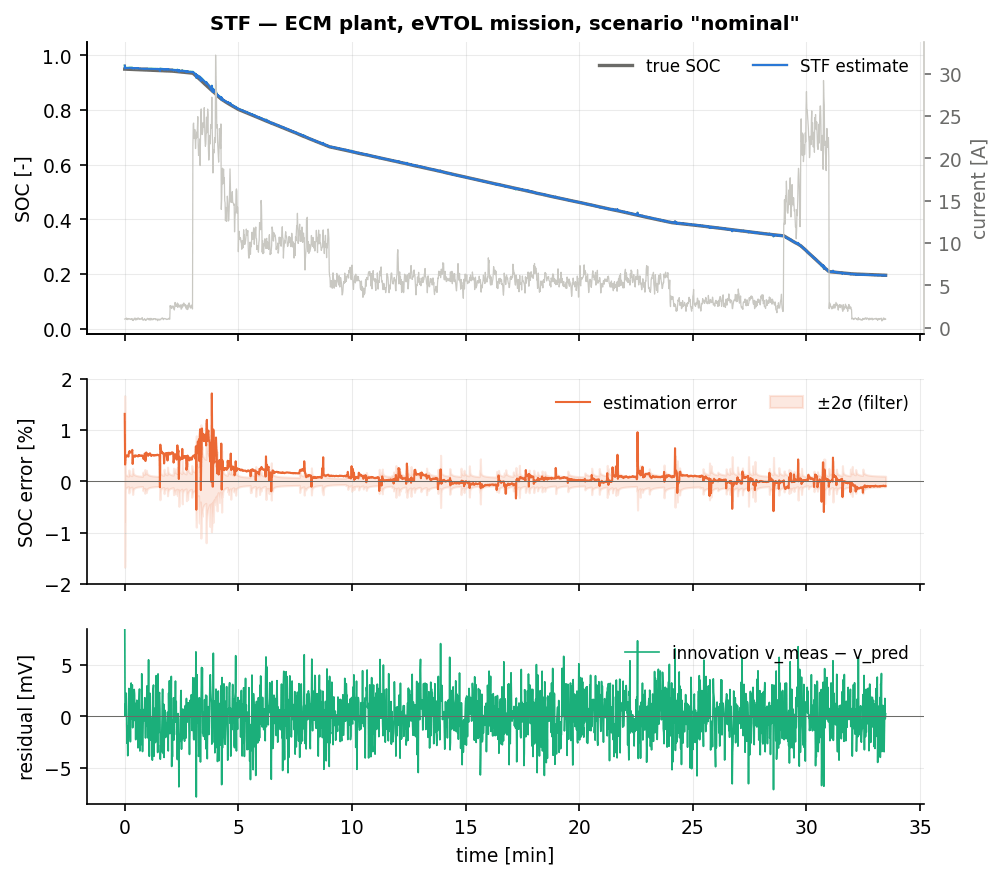
\includegraphics[width=\textwidth]{figures/cell_STF_nominal.png}
\caption{STF on the nominal eVTOL mission: true and estimated SOC (top), estimation error with the $\pm 2\sigma$ band when available (middle), voltage residual (bottom).}
\end{figure}
\begin{figure}[H]\centering
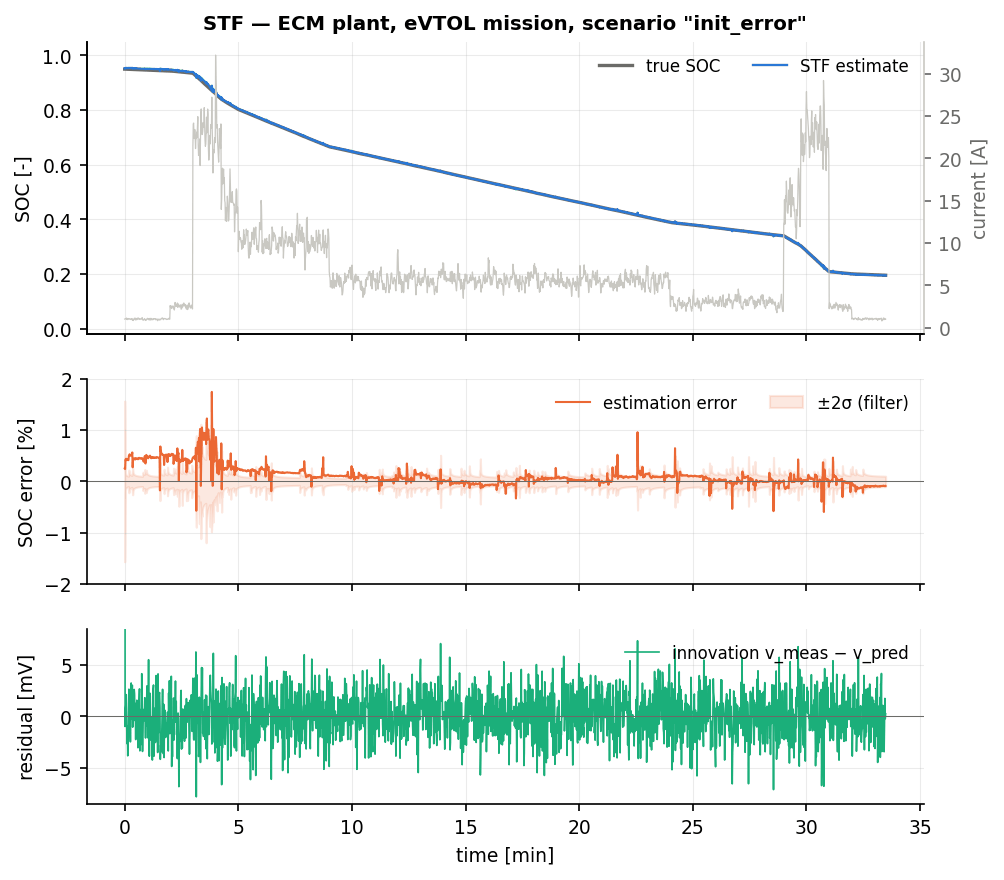
\includegraphics[width=\textwidth]{figures/cell_STF_init_error.png}
\caption{STF with a 35\,\% initial SOC error.}
\end{figure}
\begin{figure}[H]\centering
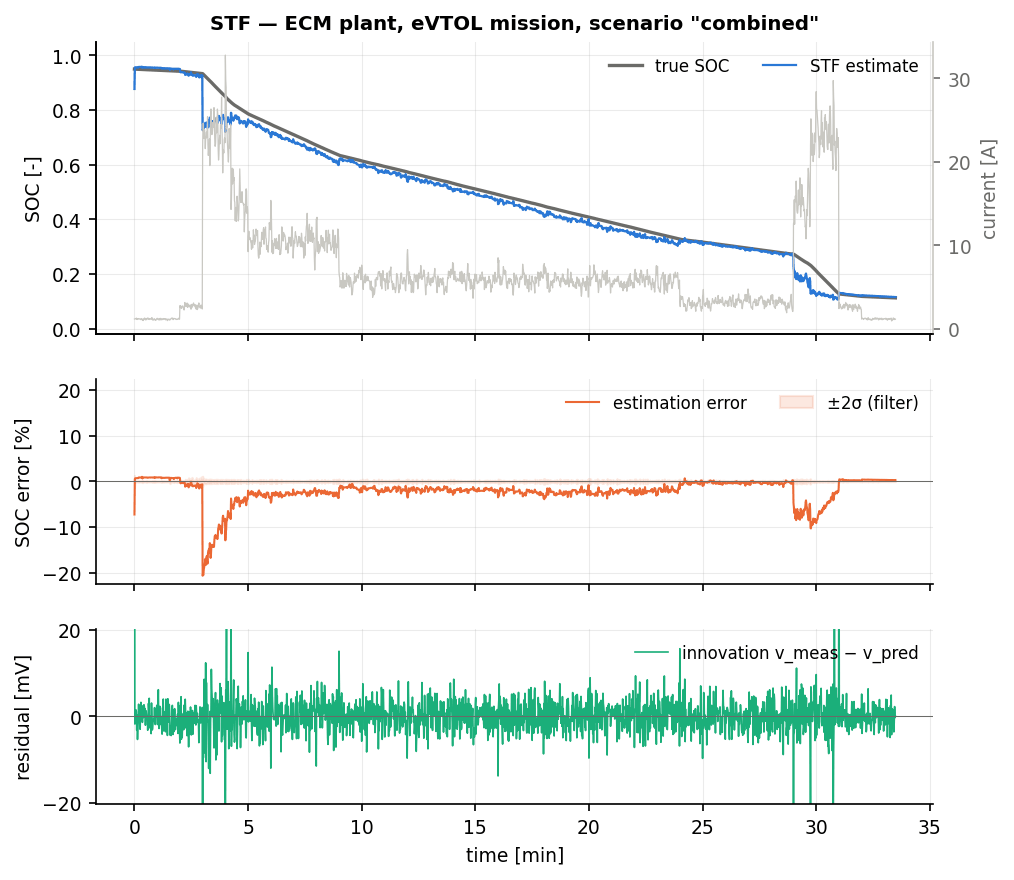
\includegraphics[width=\textwidth]{figures/cell_STF_combined.png}
\caption{STF on the \texttt{combined} scenario (25\,\% initial SOC error, \SI{150}{\milli\ampere} current bias, 2\,\% gain error, 10\,\% capacity loss with the associated resistance growth).}
\end{figure}
\begin{figure}[H]\centering
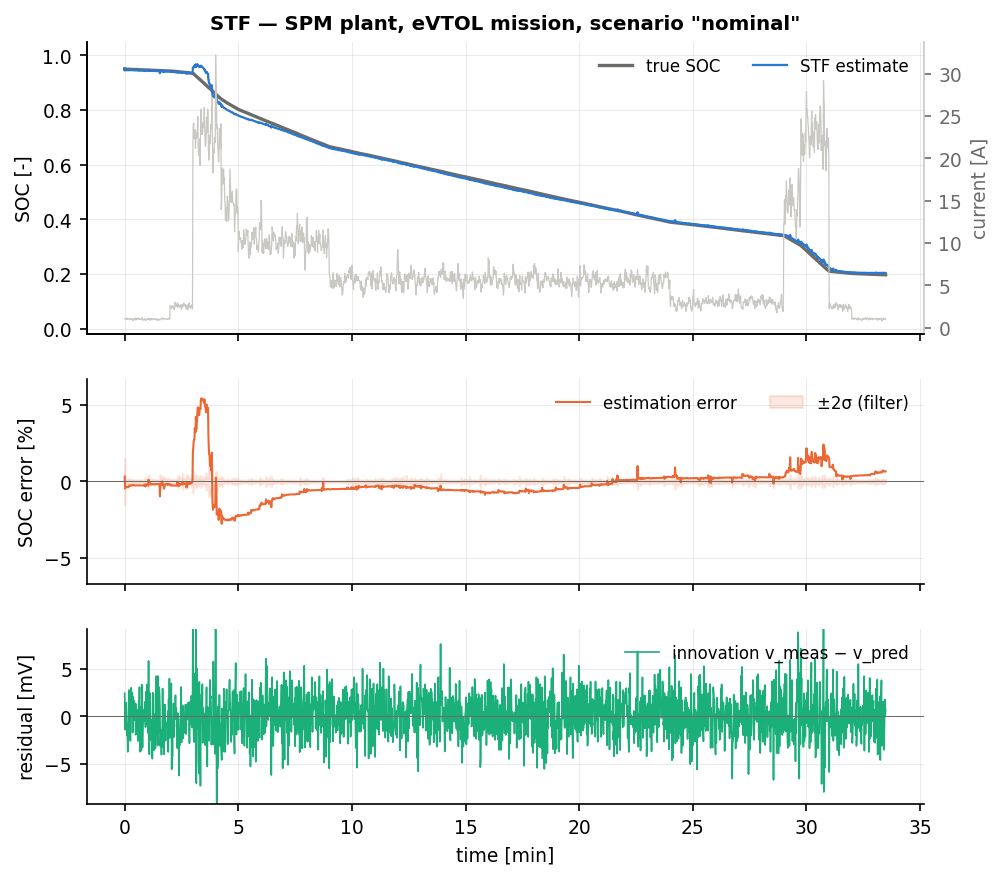
\includegraphics[width=\textwidth]{figures/cellspm_STF_nominal.png}
\caption{STF on the electrochemical (single-particle) plant, nominal mission: the estimator uses a 2-RC ECM fitted to that plant and therefore sees a structured \SI{4}{\milli\volt} residual instead of white noise.}
\end{figure}

All figures below are three-seed means in \% SOC, as tabulated above; the plain \texttt{EKF} run on
the same data is the reference (\texttt{EKF ref.} column).  For orientation, the EKF scores
$\mathrm{rmse}_{ss}$ = 0.05\,\% on \texttt{nominal}, 0.12\,\% on \texttt{noise\_step}, 0.21\,\% on
\texttt{outliers}, 0.46\,\% on \texttt{sensor\_dropout}, 1.36\,\% on \texttt{param\_mismatch},
1.52\,\% on \texttt{aged\_cell} and 12.44\,\% on \texttt{combined} (where it never converges), and
3.73\,\% on the nominal SPM mission.

\paragraph{Benign scenarios.}  \texttt{nominal}: $\mathrm{rmse}=0.24\,\%$,
$\mathrm{rmse}_{ss}=0.10\,\%$ against the EKF's $0.15\,\%$ / $0.05\,\%$.  The STF is about twice as
noisy as the EKF when nothing is wrong, with a maximum error of $2.57\,\%$ against $1.07\,\%$;
$\lambda_k$ is $1$ most of the time but fires on the manoeuvre pulses of the eVTOL profile (the
$+30\,\%$, \SI{3}{\second} current transients), where the linearisation error briefly inflates the
innovations.  Both values are comfortably inside the $2\,\%$ acceptance bound.
\texttt{init\_error} converges at $t=\SI{0}{\second}$ with $0.22\,\%$ / $0.10\,\%$.

\paragraph{Target scenario \texttt{combined}.}  This is the case the method exists for: a $25\,\%$
initial SOC error, a \SI{150}{\milli\ampere} current-sensor bias, a $2\,\%$ gain error and a
$10\,\%$ capacity loss with the associated $25\,\%$ resistance growth.  The EKF \emph{never}
converges to the $2\,\%$ band ($t_\mathrm{conv}=$ --, $\mathrm{rmse}=16.02\,\%$,
$\mathrm{rmse}_{ss}=12.44\,\%$): its covariance has collapsed, the \SI{16}{\milli\volt} voltage bias
produced by the grown $R_0$ is converted into a $12\,\%$ SOC error by the very flat OCV curve near
$\soc=0.9$, and it has no mechanism to notice.  The STF converges at $t=\SI{0}{\second}$ and holds
$\mathrm{rmse}=3.50\,\%$, $\mathrm{rmse}_{ss}=2.71\,\%$ --- a $4.6\times$ reduction of the full-run
RMSE and, more importantly, a qualitative change from "never converges" to "converges immediately".
The fading factor is doing exactly what it was designed to do: averaged over the first
\SI{200}{\second} (seed 1) $\lambda_k=8.6$, settling to $2.9$ over $[200,1000]\,\si{\second}$ and
$3.2$ over $[1000,2010]\,\si{\second}$, i.e.\ the filter permanently runs with about three times the
propagated covariance an ordinary EKF would use, which is enough to keep the gain from collapsing.
Its voltage prediction on this scenario is also the best in the family, $\mathrm{rmse}_v =
\SI{3.01}{\milli\volt}$ against the EKF's \SI{5.15}{\milli\volt} and the $\mR$-adapting filters'
\SI{14}{\milli\volt}--\SI{17}{\milli\volt}: inflating $\mP$ keeps the filter following the
measurement instead of abandoning it.

\paragraph{Other mismatch scenarios.}  \texttt{sensor\_dropout}: $\mathrm{rmse}$ $0.72\to0.49\,\%$,
$\mathrm{rmse}_{ss}$ $0.46\to0.10\,\%$ ($1.5\times$ / $4.6\times$) --- the frozen sensor produces
exactly the correlated innovation sequence the orthogonality test is looking for, although the
transient costs a maximum error of $8.63\,\%$ against the EKF's $2.27\,\%$.  On
\texttt{param\_mismatch} and \texttt{aged\_cell}, however, the STF is clearly \emph{worse} than the
EKF ($2.37\,\%$ / $1.84\,\%$ against $1.28\,\%$ / $1.36\,\%$, and $3.61\,\%$ / $2.68\,\%$ against
$1.18\,\%$ / $1.52\,\%$).  The reason is instructive: in both, the dominant model error is a
\emph{voltage} bias (wrong $R_0$), so inflating $\mP$ makes the filter trust the biased measurement
\emph{more}, and the SOC estimate is pulled further off.  The correct response there is to inflate
$\mR$, which is what the filters of \cref{ch:sagehusaakf}, \cref{ch:iaeakf} and \cref{ch:vbakf} do
--- and they achieve $0.76\,\%$--$1.30\,\%$ on those same scenarios.  \texttt{preisach} is the third
regression and the numbers moved with the corrected hysteresis sign convention: the STF now scores
$1.13\,\%$ / $0.98\,\%$ with $t_\mathrm{conv}=\SI{228}{\second}$ against the EKF's $0.58\,\%$ /
$0.20\,\%$ at \SI{16}{\second}, a factor of five worse, because a genuine un-modelled hysteresis
voltage is again an output-side error.  \texttt{cold} ($0.36\,\%$ against $0.16\,\%$) and
\texttt{current\_bias} ($0.84\,\%$ against $0.61\,\%$) are mildly worse for the same reason.

\paragraph{Where it must not be used.}  On \texttt{noise\_step} the STF is the worst estimator in the
family: $\mathrm{rmse}=1.94\,\%$, $\mathrm{rmse}_{ss}=2.34\,\%$ against the EKF's $0.18\,\%$ /
$0.12\,\%$, a factor of $20$ worse, with $\mathrm{rmse}_v$ rising to \SI{16.04}{\milli\volt}.  This is
the structural ambiguity of \eqref{eq:stf:cond} in its purest form: the tenfold rise of the
voltage-sensor noise at $t=\SI{600}{\second}$ inflates $\bm{V}_k$ by a factor of $\approx90$, the STF
reads that as model error, drives $\lambda_k$ to its covariance-cap-limited maximum, and the filter
ends up performing something close to an instantaneous OCV inversion of a \SI{20}{\milli\volt}-noisy
voltage.  \texttt{outliers} fails the same way ($1.44\,\%$ / $1.38\,\%$ against $0.52\,\%$ /
$0.21\,\%$) and is the only ECM scenario in this family where the STF does not reach the $2\,\%$ band
for \SI{60}{\second} ($t_\mathrm{conv}=$ --; no divergence).  If the sensor noise level is not known
to be constant, the STF must be combined with an $\mR$ estimator --- which is precisely the
fuzzy-supervised STF of \cite{jwo2007fuzzy} --- or replaced by an IMM (\cref{ch:imm}) that carries
both hypotheses explicitly and gets $0.05\,\%$ on \texttt{noise\_step} and $1.02\,\%$ on
\texttt{combined}.

\paragraph{Cost.}  \SI{532}{\nano\second}/step against the EKF's \SI{478}{\nano\second}/step, with no
buffers.

\paragraph{Electrochemical (SPM) plant.}  Here the picture inverts completely, and the SPM rows are
the strongest argument in this chapter for the method.  With a 2-RC ECM fitted to the single-particle
plant the residual is a structured, slowly varying \SI{4}{\milli\volt} signal --- genuine model error,
not sensor noise --- and that is exactly the hypothesis the orthogonality condition
\eqref{eq:stf:r2} is built on.  The STF reaches $\mathrm{rmse}_{ss}=\mathbf{0.66\,\%}$ on the nominal
SPM mission against the EKF's $3.73\,\%$, a $\mathbf{5.7\times}$ improvement, and against
$3.02\,\%$--$3.33\,\%$ for all four $\mR$-adapting filters, which improve on the EKF by barely
$10$--$20\,\%$.  The explanation is the one the ECM rows hinted at, seen from the other side.
Covariance matching cannot ask \emph{why} the residuals are large; concluding "noisy sensor" and
lowering the gain hands SOC to the coulomb integrator, and on this plant the integrator is the faulty
component (the fitted capacity and efficiency do not reproduce the true lithium inventory), so the
estimate parks at a $3\,\%$ offset.  The measurement is the reliable part --- the ECM's
$\ocv(\soc)$ map \emph{was} fitted to this plant --- so the useful response is to shorten the
filter's memory until recent measurements outweigh the accumulated model, which is what
$\lambda_k>1$ does.  Under structured model error, inflating $\mP$ (trusting the measurement more)
beats inflating $\mR$ (trusting it less), and the ECM \texttt{aged\_cell} row above is the mirror
image: there the error lived in the output map, and the ordering of the two families reverses.  The
advantage carries across the SPM scenarios --- \texttt{init\_error} $3.81\to0.66\,\%$,
\texttt{current\_bias} $5.69\to0.72\,\%$ ($7.9\times$), \texttt{sensor\_dropout} $5.31\to0.66\,\%$
($8.0\times$), \texttt{hot} $2.16\to0.74\,\%$, \texttt{param\_mismatch} $3.13\to1.75\,\%$ --- with the
two familiar exceptions where the disturbance really \emph{is} on the sensor: SPM
\texttt{noise\_step} ($2.53\,\%$ against $3.30\,\%$, an improvement but far behind Fading-EKF's
$0.43\,\%$) and SPM \texttt{outliers} ($1.64\,\%$ against $1.99\,\%$, $t_\mathrm{conv}=$ --).  SPM
\texttt{cold} is the one genuine failure ($5.12\,\%$ against $7.35\,\%$ in steady state but a
\SI{966}{\second} convergence time and a $17.88\,\%$ maximum error): at \SI{-10}{\celsius} the
diffusion time constant grows beyond \SI{2000}{\second}, the innovation sequence is correlated over
the whole mission, and the fading factor stays large enough to make the estimate jumpy.

\section{Summary}
The strong tracking filter adds one scalar to the EKF and buys a qualitative improvement in
re-convergence after model mismatch: on the hardest scenario of this benchmark it turns "never
converges, $12\,\%$ steady-state SOC error" into "converges immediately, $2.7\,\%$".  Use it when the
plant model is the suspect part and the sensor model is trustworthy --- manoeuvre changes, ageing,
parameter drift, stuck sensors.  Do not use it when the measurement-noise level itself can change,
because the orthogonality condition cannot tell the two apart and the filter will respond to a
noisier sensor by trusting it more.  Its best case in this benchmark is the electrochemical plant, where the 2-RC model leaves a
structured \SI{4}{\milli\volt} residual and the STF reaches $0.66\,\%$ against the EKF's
$3.73\,\%$ --- a $5.7\times$ gain, while every $\mR$-adapting filter manages only $10$--$20\,\%$,
because under model error the right move is to trust the measurement more, not less.  Never use it
without a covariance bound on a plant with weakly observable states: the scalar inflation is blind to
observability, and on this cell model the unbounded version reaches NaN in under \SI{200}{\second}.

% Copyright 2026 Sreeram Anil
% SPDX-License-Identifier: CC-BY-4.0
% =============================================================================
%  Fading-memory (exponentially weighted) extended Kalman filter
% =============================================================================
\chapter{Fading-memory extended Kalman filter (Fading-EKF)}
\label{ch:fadingekf}

\section*{At a glance}
\begin{tabular}{@{}l>{\raggedright\arraybackslash}p{0.76\textwidth}@{}}
Family & Adaptive Kalman \\
Header & \texttt{include/estkit/filters/fading\_kf.hpp} \\
Registered name & \texttt{Fading-EKF} \\
State dimension & $n_x = 4$ (cell model) --- generic in $n_x, n_u, n_y$ \\
Cost per step & EKF $+\,n_x^2$ multiplies $+\,\mathcal{O}(n_x^2)$ clamp; $\approx 500$\,ns/step, no heap \\
Primary references & \cite{sorenson1971fading,simon2006,andersonmoore1979,jazwinski1970} \\
\end{tabular}

\section{Motivation and aerospace/BMS relevance}
The Kalman filter weights every past measurement equally.  That is optimal if the model is exactly
right for the whole record, and it is the wrong thing to do otherwise: after a few hundred samples
the filter has accumulated so much (apparent) information that the gain has fallen to its
steady-state value and the estimate becomes a slave to the model.  Any un-modelled bias --- a
current-sensor offset, a capacity that has faded since the look-up tables were written, a series
resistance that has grown --- then produces an estimation error that decays with the filter's very
long closed-loop time constant, if it decays at all.

Sorenson and Sacks \cite{sorenson1971fading} proposed the simplest possible fix: discount old data
geometrically.  The resulting "fading-memory" or "exponentially data-weighted" filter is the Kalman
filter with a single line changed, $\Pminus = \alpha^2\mF\Pplus\mF^\T+\mQ$ with $\alpha\ge1$, and
Simon presents it in exactly this form \cite[Sec.~7.4]{simon2006}.  It is not adaptive in the sense
of estimating anything --- $\alpha$ is a fixed design parameter --- but it belongs in this chapter
because it is the limiting case of the strong tracking filter with $\lambda_k$ frozen at a constant,
and because it is by far the most widely deployed member of the family: a great many industrial
Kalman filters ship with a small covariance inflation whose provenance is exactly this argument.

For a BMS the appeal is practical.  A flight-worthy SOC estimator must re-converge after the pack has
been swapped, after a firmware reset with a stale SOC, and it must not slowly walk away from the
truth as the cell ages between calibrations.  A fading-memory filter guarantees a gain floor and
therefore a bounded error-rejection time constant, at the cost of a permanently higher noise floor.
The trade is explicit and can be certified: a designer can state "this filter forgets everything
older than \SI{25}{\second}", which is a much easier statement to defend than "this filter is
optimal for the model we identified two years ago".

\section{Problem statement and assumptions}
The plant is \eqref{eq:sh:proc}--\eqref{eq:sh:meas}.  Rather than the unweighted maximum-likelihood
criterion behind the Kalman filter, consider the exponentially weighted one
\begin{equation}
J_k = \sum_{j=1}^{k}\alpha^{-2(k-j)}\Big[\bm{e}_j^\T\mR_j\inv\bm{e}_j + \vw_{j-1}^\T\mQ_{j-1}\inv\vw_{j-1}\Big]
      + \alpha^{-2k}\,\tilde{\vx}_0^\T\mP_0\inv\tilde{\vx}_0 ,
\label{eq:fm:cost}
\end{equation}
where $\alpha\ge1$ and $\tilde{\vx}_0=\vx_0-\xhat_0$.  A datum $j$ steps in the past enters with
weight $\alpha^{-2j}$, so the effective number of samples retained is
\begin{equation}
\tau = \sum_{j\ge0}\alpha^{-2j}\Big/1 = \frac{1}{1-\alpha^{-2}} \approx \frac{1}{2\ln\alpha}
\quad\text{samples, for } \alpha\to1^+ .
\label{eq:fm:tau}
\end{equation}

\begin{assumption}\label{as:fm:mismatch}
The dominant error source is a slowly varying, un-modelled deterministic bias rather than an
incorrect noise level, so that discarding old data is beneficial.
\end{assumption}
\begin{assumption}\label{as:fm:obs}
Every state direction is observable within $\tau$ samples --- see \cref{sec:fm:cap} for what happens
when this fails.
\end{assumption}

\section{Derivation}

\subsection{From the weighted cost to the recursion}
Minimising \eqref{eq:fm:cost} is the same as minimising the unweighted cost for a modified system in
which every covariance is scaled by the discount.  Formally, substitute
$\vx'_j = \alpha^{-j}\vx_j$, $\vy'_j=\alpha^{-j}\vy_j$, $\vw'_j=\alpha^{-j}\vw_j$,
$\vv'_j=\alpha^{-j}\vv_j$; then \eqref{eq:fm:cost} becomes the ordinary quadratic cost of the
transformed system
\begin{equation}
\vx'_{j} = \alpha^{-1}\mF_{j-1}\vx'_{j-1} + \vw'_{j-1},\qquad
\vy'_j = \mH_j\vx'_j+\vv'_j ,
\label{eq:fm:transformed}
\end{equation}
with $\mQ'_j=\alpha^{-2j}\mQ_j$ and $\mR'_j=\alpha^{-2j}\mR_j$.  Running a Kalman filter on
\eqref{eq:fm:transformed}, transforming back with $\mP_j = \alpha^{2j}\mP'_j$ and simplifying gives
the time update
\begin{equation}
\boxed{\;\Pminus_k = \alpha^2\,\mF_{k-1}\Pplus_{k-1}\mF_{k-1}^\T + \mQ_{k-1}\;}
\label{eq:fm:pred}
\end{equation}
with the state prediction, gain and measurement update unchanged
\cite{sorenson1971fading}\cite[Sec.~7.4]{simon2006}.  Setting $\alpha=1$ recovers the ordinary EKF.

\subsection{Effect on the steady-state gain}
It is worth computing what \eqref{eq:fm:pred} actually buys.  Take a scalar observable direction with
$\mF=1$, $\mH=g$, process-noise variance $q$ and measurement-noise variance $r$.  The steady-state
prediction variance $X$ of the fading filter satisfies
$X = \alpha^2 X\,r/(g^2X+r) + q$, i.e.
\begin{equation}
g^2X^2 - X\big[(\alpha^2-1)r + q g^2\big] - qr = 0 ,
\label{eq:fm:fix}
\end{equation}
whose positive root, for $(\alpha^2-1)r \gg qg^2$, is $X \approx (\alpha^2-1)r/g^2$, independent of
$q$.  The gain floor is therefore
\begin{equation}
K_\infty \;=\; \frac{gX}{g^2X+r} \;\approx\; \frac{\alpha^2-1}{\alpha^2}\cdot\frac{1}{g}
\quad\text{when } (\alpha^2-1)\gg qg^2/r ,
\label{eq:fm:gainfloor}
\end{equation}
so the closed-loop error time constant is bounded by $1/(K_\infty g)\approx \alpha^2/(\alpha^2-1)
\approx \tau$ samples --- the memory length, as expected.  For the cell model at the flat part of
the OCV curve ($g\approx0.2$), $q_{\soc\soc}=10^{-10}$, $r=4.4\times10^{-6}$, the plain EKF
($\alpha=1$) gives $X = \sqrt{qr}/g = 1.5\times10^{-7}$ and $K_\infty=4.8\times10^{-3}$, i.e.\ an
error time constant of $\approx\SI{150}{\second}$; $\alpha=1.002$ gives
$X=4.4\times10^{-6}\cdot 4\times10^{-3}/0.04 = 4.4\times10^{-7}$ and a time constant of
$\approx\SI{25}{\second}$, a six-fold speed-up of bias rejection.  The cost is a
$\sqrt{6}\approx2.4$-fold increase in the noise-driven error, which is negligible here because the
noise term is not what limits the SOC estimate.

\subsection{$\alpha$ is a per-sample quantity}
\eqref{eq:fm:tau} makes the essential point that is often glossed over: $\alpha$ discounts per
\emph{sample}, so its numerical value is meaningless without the sample rate.  The textbook values
$\alpha=1.01$--$1.05$ \cite[Sec.~7.4]{simon2006} correspond to $\tau=50$ down to $10$ samples.  At
the \SI{10}{\hertz} rate of this benchmark that is \SI{5}{\second} to \SI{1}{\second} of memory,
far shorter than the cell's slow RC time constant $\tau_2=\SI{120}{\second}$ and shorter even than
the fast one, $\tau_1=\SI{5}{\second}$ --- the filter would forget the very dynamics it is supposed
to be estimating.  The default used here is $\alpha=1.002$, i.e.\ $\tau=250$ samples
$=\SI{25}{\second}$: long compared with $\tau_1$, short compared with the \SI{2010}{\second} mission,
and comparable with the exponential windows chosen for the covariance-matching filters
($1/(1-b)=200$ samples for Sage--Husa, $N=80$ for IAE).

\subsection{Covariance limiting is not optional}
\label{sec:fm:cap}
Equation \eqref{eq:fm:pred} multiplies \emph{every} direction of the state space by $\alpha^2$,
including those that the measurement barely constrains.  \cref{as:fm:obs} is what makes the
recursion well posed; when it fails, $\mP$ grows like $\alpha^{2k}$ in the offending direction
without bound.  For the ECM the offending direction is the $(\soc,h)$ combination, whose
observability Gramian over a window of $K$ samples grows only as $K^3$ (the hysteresis and SOC modes
differ by $1.5\times10^{-3}$ per sample and are seen through a single output).  This is not a
theoretical concern: with $\alpha=1.005$ and no bound, the measured $P_{hh}$ on the
\texttt{nominal} scenario rises from $0.25$ to $11$ within \SI{50}{\second} and to $19$ by
\SI{100}{\second}, the hysteresis estimate saturates at its constraint $h=1$, the cross term
$P_{v_1h}$ then flips the sign of the $v_1$ gain, and $v_1$ diverges to $10^{91}$ and then to NaN by
$t=\SI{200}{\second}$.  Every $\alpha>1$ diverges eventually; only the time scale changes.

The implementation therefore bounds the prediction covariance,
\begin{equation}
P^-_{k,ii}\le c_P P_{0,ii},\qquad
P^-_{k,ij}\gets P^-_{k,ij}\sqrt{P^{\text{new}}_{ii}/P^{\text{old}}_{ii}} \ \ \forall j ,
\label{eq:fm:cap}
\end{equation}
which caps each state's predicted standard deviation at $\sqrt{c_P}$ times its initial value while
preserving all correlation coefficients (and hence positive semi-definiteness, since the
Cauchy--Schwarz bound $|P_{ij}|\le\sqrt{P_{ii}P_{jj}}$ is inherited).  Covariance limiting is the
classical remedy for exactly this failure \cite[Sec.~4.4]{andersonmoore1979}\cite[Sec.~7.4]{simon2006}.

\section{Algorithm}
\begin{algorithm}[H]
\caption{Fading-EKF --- one sampling period}
\begin{algorithmic}[1]
\Require $\xplus_{k-1},\Pplus_{k-1},\vu_{k-1},\vy_k,\vu_k,\alpha,c_P$
\State \textbf{Time update:} $\mF\gets\partial f/\partial\vx|_{\xplus_{k-1}}$;\quad $\xminus_k\gets f(\xplus_{k-1},\vu_{k-1})$
\State \quad $\Pminus_k\gets\alpha^2\,\mF\Pplus_{k-1}\mF^\T+\mQ(\xminus_k,\vu_{k-1})$;\quad symmetrise;\quad apply \eqref{eq:fm:cap}
\State \textbf{Innovation:} $\mH\gets\partial h/\partial\vx|_{\xminus_k}$;\quad $\bm{e}_k\gets\vy_k-h(\xminus_k,\vu_k)$
\State \textbf{Gain:} $\mS_k\gets\mH\Pminus_k\mH^\T+\mR_k$;\quad $\mK_k\gets\Pminus_k\mH^\T\mS_k\inv$
       \Comment{skip the update if $\mK_k$ is not finite}
\State \textbf{Update:} $\xplus_k\gets\xminus_k+\mK_k\bm{e}_k$;\quad
       $\Pplus_k\gets(\mI-\mK_k\mH)\Pminus_k(\mI-\mK_k\mH)^\T+\mK_k\mR_k\mK_k^\T$
\State \textbf{Constrain:} $\xplus_k\gets\mathrm{constrain}(\xplus_k)$
\Ensure $\xplus_k,\Pplus_k$
\end{algorithmic}
\end{algorithm}

\section{Application to the battery model}
No part of the algorithm is battery-specific: $\alpha$ multiplies the propagated covariance and the
cap is expressed relative to $\mP_0$, which the benchmark supplies as
$\diag(\sigma_{z0}^2,\,2^2,\,5^2,\,500^2)\,\si{\milli\volt}^2$-scaled entries, i.e.\
$\diag(0.01,\,4\times10^{-6},\,2.5\times10^{-5},\,0.25)$.  With $c_P=0.01$ the caps are
$\sigma_\soc\le0.01$, $\sigma_{v_1}\le\SI{0.2}{\milli\volt}$, $\sigma_{v_2}\le\SI{0.5}{\milli\volt}$,
$\sigma_h\le0.05$.  The SOC cap is the one that matters: at $P_{\soc\soc}=10^{-4}$ the gain is
already at the OCV-inversion limit $1/g$, so the cap costs nothing in tracking ability while
stopping the hysteresis direction from running away.

$\alpha$ and $c_P$ were selected on a grid $\alpha\in\{1.002,1.005,1.01,1.02,1.05\}\times
c_P\in\{0.003,0.01,0.03\}$.  The metrics vary smoothly; $\alpha=1.002$, $c_P=0.01$ is the best
compromise and was adopted.  Larger $\alpha$ costs accuracy on every benign scenario without buying
anything on \texttt{combined} (in the single-seed development sweep $\alpha=1.05$ gave
$3.30\,\%$ / $2.74\,\%$ there versus $0.92\,\%$ / $1.16\,\%$ at $\alpha=1.002$), which is the
quantitative statement of the sample-rate
argument above.

\section{Implementation notes}
\begin{itemize}[leftmargin=1.4em]
\item \textbf{Cost.}  One extra scalar multiply of an $n_x\times n_x$ matrix and the diagonal clamp:
      measured \SI{501}{\nano\second}/step against \SI{478}{\nano\second}/step for the EKF ---
      a $5\,\%$ overhead, and the cheapest filter of this family.  On a \SI{400}{\mega\hertz}
      Cortex-M7 this is roughly \SI{7}{\micro\second}/step.  Memory overhead: $n_x$ reals for the caps.
\item \textbf{Deterministic.}  Unlike the covariance-matching filters, nothing here depends on the
      data, so the gain sequence is a deterministic function of the trajectory.  This makes the
      filter much easier to analyse and to certify: worst-case error bounds can be computed offline.
\item \textbf{Joseph form and symmetrisation} are used exactly as in the EKF; a non-finite gain
      causes the update to be skipped.
\item \textbf{float32.}  The single-precision build reproduces the double-precision metrics to three
      digits on all twelve scenarios with no divergence.
\item \textbf{Limitations.}  $\alpha$ is a fixed design choice: the filter pays the noise penalty all
      the time, whether or not the model is wrong.  If the mismatch is intermittent, the STF
      (\cref{ch:stf}) or the IMM (\cref{ch:imm}), which switch the inflation on only when the
      innovations demand it, are better.  The filter also does nothing about a changing
      measurement-noise level.
\end{itemize}

\section{Benchmark results}
% Copyright 2026 Sreeram Anil
% SPDX-License-Identifier: CC-BY-4.0
\begin{table}[H]\centering\footnotesize\setlength{\tabcolsep}{4pt}
\caption{Fading-EKF: cell-level benchmark on the eVTOL mission (mean over seeds; RMSE and max error in \% SOC; $t_\mathrm{conv}$: first time the error stays below 2\,\% for 60\,s, -- = never; EKF reference: steady-state RMSE of the plain EKF on the same data).}\label{tab:cell_FadingEKF}
\begin{tabular}{llrrrrrcrr}\toprule
plant & scenario & RMSE & RMSE$_\mathrm{ss}$ & max & $t_\mathrm{conv}$ [s] & RMSE$_v$ [mV] & div. & EKF ref. & ns/step \\ \midrule
ECM & nominal & 0.21 & 0.05 & 1.02 & 0 & 0.77 & no & 0.05 & 501 \\
ECM & init\_error & 0.18 & 0.05 & 0.59 & 0 & 2.12 & no & 0.05 & 500 \\
ECM & current\_bias & 0.70 & 0.66 & 1.56 & 0 & 0.83 & no & 0.61 & 502 \\
ECM & noise\_step & 0.24 & 0.16 & 1.02 & 0 & 2.56 & no & 0.12 & 499 \\
ECM & outliers & 0.25 & 0.09 & 2.35 & 0 & 1.84 & no & 0.21 & 502 \\
ECM & cold & 0.33 & 0.25 & 1.20 & 0 & 1.88 & no & 0.16 & 500 \\
ECM & hot & 0.19 & 0.02 & 0.98 & 0 & 0.52 & no & 0.03 & 501 \\
ECM & aged\_cell & 1.67 & 1.78 & 4.68 & 0 & 4.12 & no & 1.52 & 500 \\
ECM & param\_mismatch & 1.27 & 1.31 & 3.54 & 0 & 3.05 & no & 1.36 & 500 \\
ECM & sensor\_dropout & 0.21 & 0.05 & 1.42 & 0 & 1.67 & no & 0.46 & 499 \\
ECM & preisach & 1.08 & 0.86 & 2.87 & 224 & 0.79 & no & 0.20 & 502 \\
ECM & combined & 0.93 & 1.18 & 7.36 & 0 & 5.16 & no & 12.44 & 503 \\
\midrule
SPM & nominal & 0.60 & 0.36 & 1.80 & 0 & 1.11 & no & 3.73 & 465 \\
SPM & init\_error & 0.77 & 0.48 & 1.90 & 0 & 2.21 & no & 3.81 & 479 \\
SPM & current\_bias & 0.89 & 0.87 & 2.09 & 0 & 1.21 & no & 5.69 & 476 \\
SPM & noise\_step & 0.64 & 0.43 & 1.80 & 0 & 2.74 & no & 3.30 & 482 \\
SPM & outliers & 0.69 & 0.45 & 2.49 & 0 & 2.04 & no & 1.99 & 468 \\
SPM & cold & 3.36 & 3.45 & 7.10 & 326 & 4.94 & no & 7.35 & 476 \\
SPM & hot & 0.55 & 0.35 & 1.27 & 0 & 0.72 & no & 2.16 & 479 \\
SPM & param\_mismatch & 2.17 & 1.95 & 4.45 & 0 & 2.19 & no & 3.13 & 475 \\
SPM & sensor\_dropout & 0.52 & 0.31 & 2.69 & 0 & 2.00 & no & 5.31 & 477 \\
\bottomrule\end{tabular}\end{table}

\begin{figure}[H]\centering
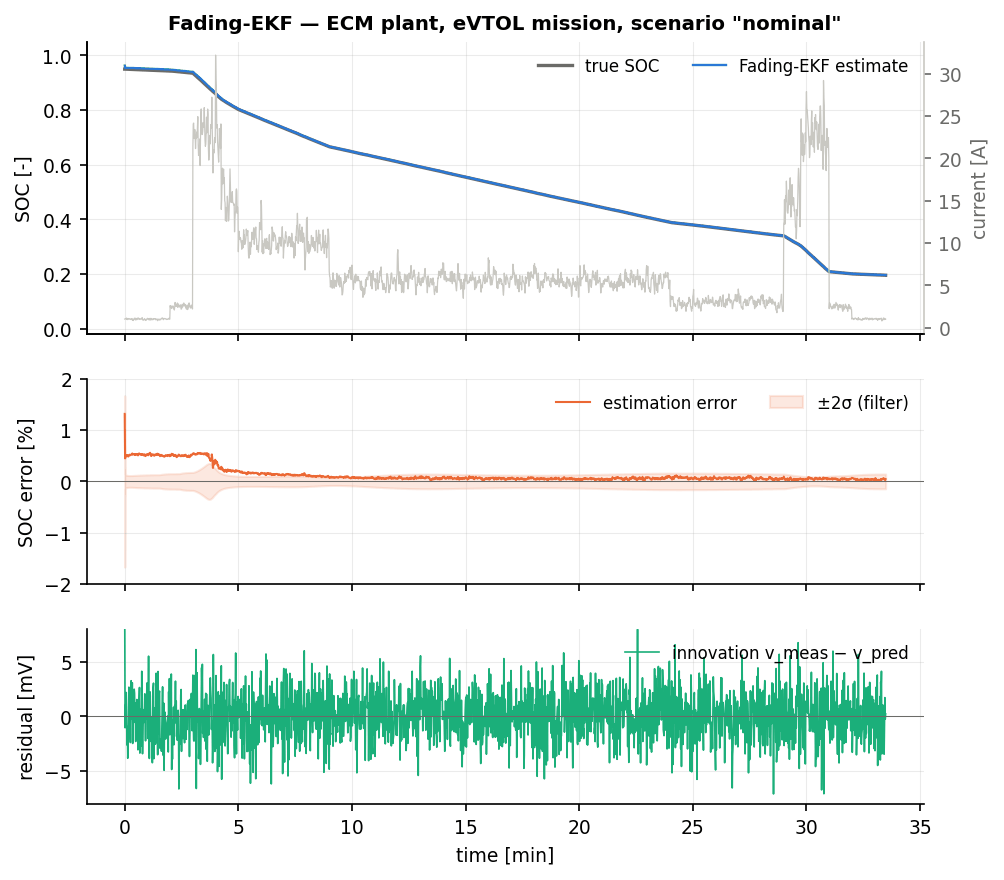
\includegraphics[width=\textwidth]{figures/cell_FadingEKF_nominal.png}
\caption{Fading-EKF on the nominal eVTOL mission: true and estimated SOC (top), estimation error with the $\pm 2\sigma$ band when available (middle), voltage residual (bottom).}
\end{figure}
\begin{figure}[H]\centering
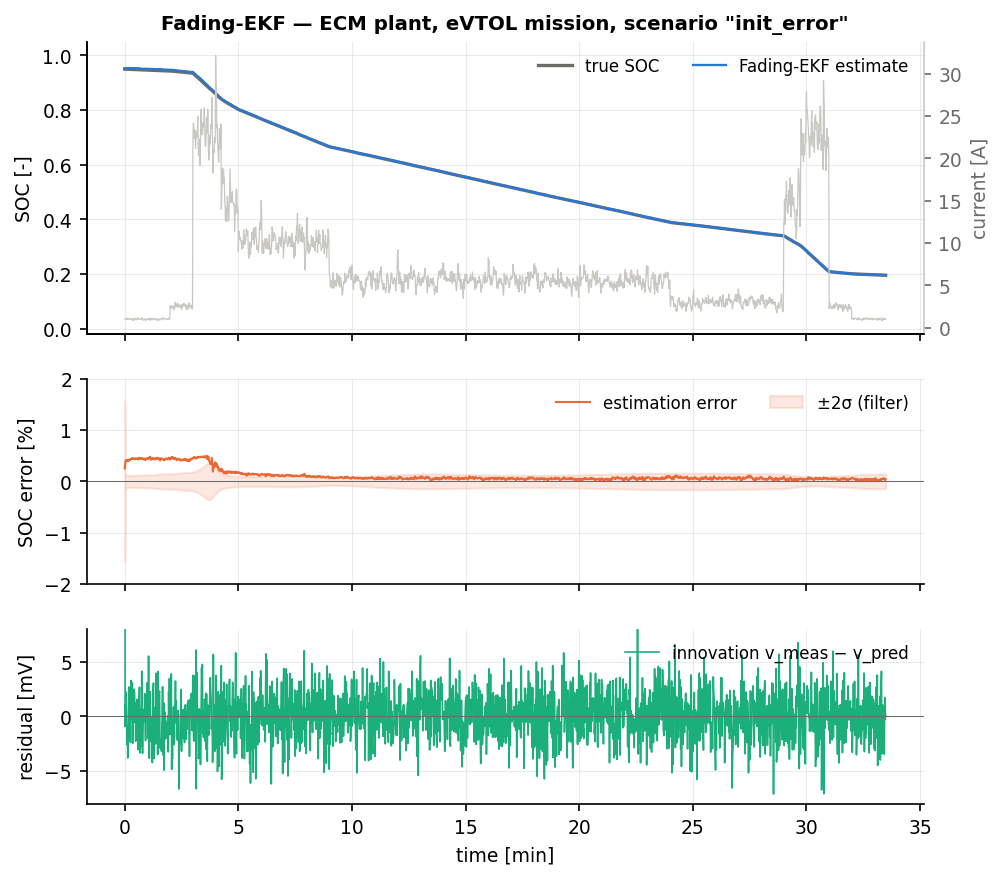
\includegraphics[width=\textwidth]{figures/cell_FadingEKF_init_error.png}
\caption{Fading-EKF with a 35\,\% initial SOC error.}
\end{figure}
\begin{figure}[H]\centering
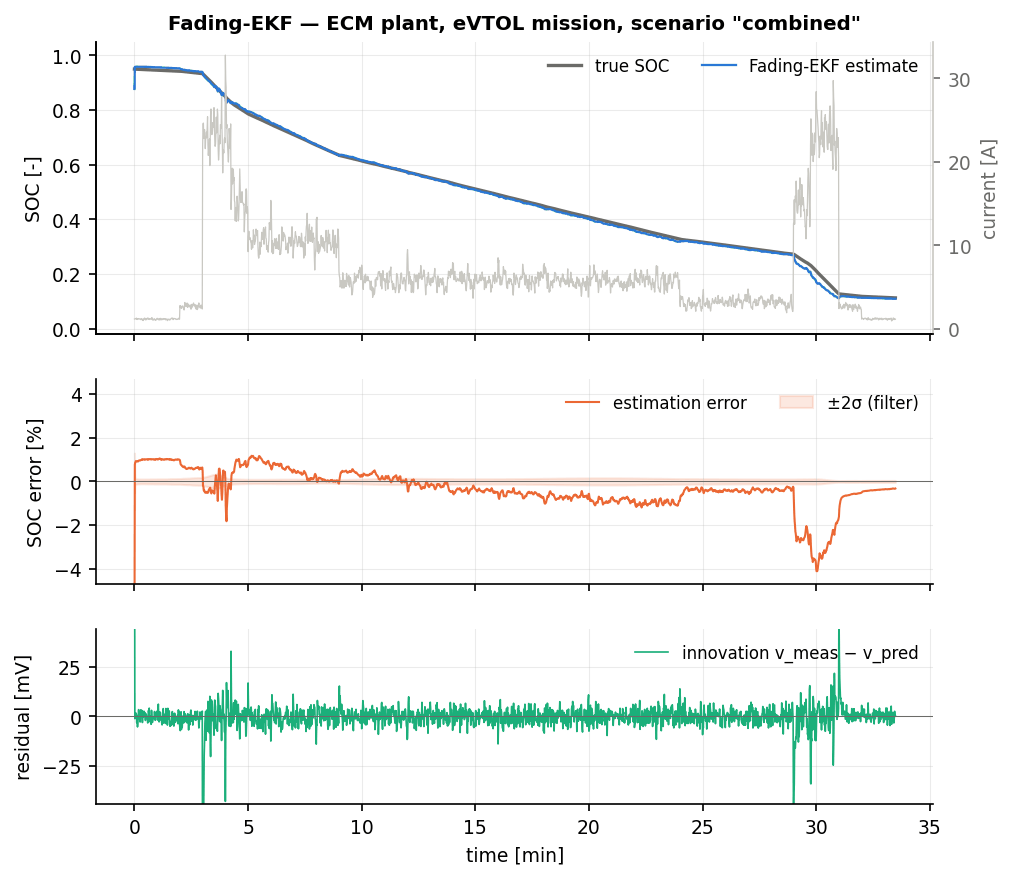
\includegraphics[width=\textwidth]{figures/cell_FadingEKF_combined.png}
\caption{Fading-EKF on the \texttt{combined} scenario (25\,\% initial SOC error, \SI{150}{\milli\ampere} current bias, 2\,\% gain error, 10\,\% capacity loss with the associated resistance growth).}
\end{figure}
\begin{figure}[H]\centering
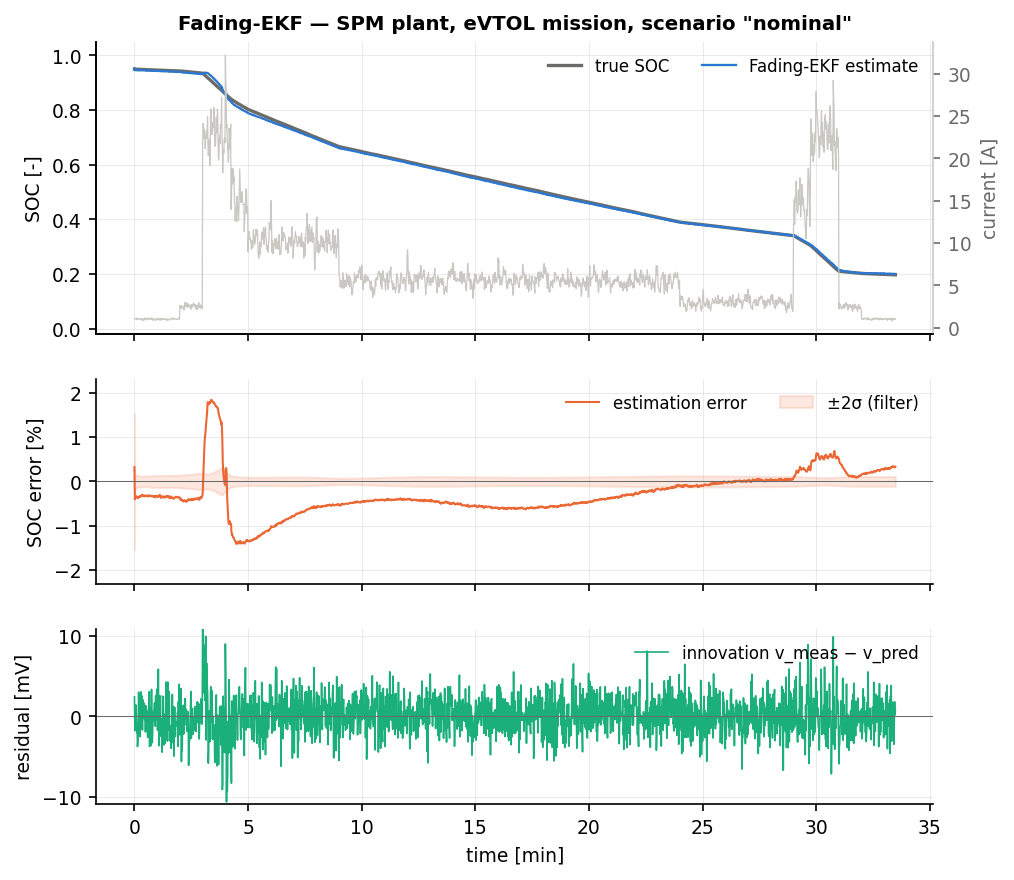
\includegraphics[width=\textwidth]{figures/cellspm_FadingEKF_nominal.png}
\caption{Fading-EKF on the electrochemical (single-particle) plant, nominal mission: the estimator uses a 2-RC ECM fitted to that plant and therefore sees a structured \SI{4}{\milli\volt} residual instead of white noise.}
\end{figure}

All figures below are three-seed means in \% SOC, as tabulated above; the plain \texttt{EKF} run on
the same data is the reference (\texttt{EKF ref.} column).  For orientation, the EKF scores
$\mathrm{rmse}_{ss}$ = 0.05\,\% on \texttt{nominal}, 0.12\,\% on \texttt{noise\_step}, 0.21\,\% on
\texttt{outliers}, 0.46\,\% on \texttt{sensor\_dropout}, 1.36\,\% on \texttt{param\_mismatch},
1.52\,\% on \texttt{aged\_cell} and 12.44\,\% on \texttt{combined} (where it never converges), and
3.73\,\% on the nominal SPM mission.

\paragraph{Benign scenarios.}  \texttt{nominal}: $\mathrm{rmse}=0.21\,\%$,
$\mathrm{rmse}_{ss}=0.05\,\%$, identical to the EKF's $0.15\,\%$ / $0.05\,\%$ in steady state and with
a \emph{smaller} maximum error ($1.02\,\%$ against $1.07\,\%$).  The six-fold larger gain predicted by
\eqref{eq:fm:gainfloor} costs nothing measurable here because the noise term is not what limits the
SOC estimate on this plant.  \texttt{init\_error}: $\mathrm{rmse}=0.18\,\%$,
$\mathrm{rmse}_{ss}=0.05\,\%$, converging at $t=\SI{0}{\second}$, again with the smallest maximum
error of the whole family ($0.59\,\%$ against the EKF's $0.62\,\%$) because the larger gain removes the
initial offset faster.

\paragraph{Target scenario \texttt{combined}.}  The Fading-EKF is the best of the eight adaptive
filters on the benchmark's hardest ECM scenario.  The EKF never converges ($t_\mathrm{conv}=$ --,
$\mathrm{rmse}=16.02\,\%$, $\mathrm{rmse}_{ss}=12.44\,\%$); the Fading-EKF converges at
$t=\SI{0}{\second}$ with $\mathrm{rmse}=\mathbf{0.93\,\%}$ and
$\mathrm{rmse}_{ss}=\mathbf{1.18\,\%}$ --- a $\mathbf{17\times}$ reduction of the full-run RMSE and a
$\mathbf{10.5\times}$ reduction of the steady-state RMSE, with the maximum error down from $29.64\,\%$
to $7.36\,\%$.  The explanation is \eqref{eq:fm:gainfloor}: the $25\,\%$ resistance growth puts a
\SI{16}{\milli\volt} bias on the predicted voltage, which the flat OCV curve near $\soc=0.9$ amplifies
into a large SOC bias of gain-dependent magnitude; a six-fold larger gain floor divides the resulting
steady-state SOC bias by roughly the same factor, and the \SI{25}{\second} memory means the
current-bias-driven drift is corrected six times faster as well.  It also keeps the best voltage
prediction of the family on this scenario after the STF ($\mathrm{rmse}_v=\SI{5.16}{\milli\volt}$,
essentially the EKF's \SI{5.15}{\milli\volt}, against \SI{14}{\milli\volt}--\SI{17}{\milli\volt} for
the $\mR$-adapting filters).

\paragraph{Other mismatch scenarios.}  \texttt{sensor\_dropout}: $\mathrm{rmse}$ $0.72\to0.21\,\%$,
$\mathrm{rmse}_{ss}$ $0.46\to0.05\,\%$ --- a $3.4\times$ / $9.2\times$ improvement and the joint best
in the family, because the filter simply forgets the \SI{15}{\second} of frozen data within a
comparable time.  \texttt{param\_mismatch}: $1.28\to1.27\,\%$ and $1.36\to1.31\,\%$, essentially a
draw.  \texttt{outliers}: $0.52\to0.25\,\%$ and $0.21\to0.09\,\%$, a useful $2.1\times$ / $2.3\times$
even though nothing in the design targets impulsive noise --- the shorter memory simply flushes each
spike out faster.

\paragraph{Where it costs.}  \texttt{aged\_cell} is worse than the EKF ($\mathrm{rmse}=1.67\,\%$,
$\mathrm{rmse}_{ss}=1.78\,\%$ against $1.18\,\%$ / $1.52\,\%$), for the same reason the STF is worse
there: the dominant error is a voltage bias, and a larger gain makes a biased measurement more
influential, not less.  \texttt{current\_bias} is also slightly worse ($0.66\,\%$ against $0.61\,\%$)
and \texttt{cold} likewise ($0.25\,\%$ against $0.16\,\%$).  The clearest regression is
\texttt{preisach}, whose numbers moved with the corrected hysteresis sign convention: $1.08\,\%$ /
$0.86\,\%$ with $t_\mathrm{conv}=\SI{224}{\second}$ against the EKF's $0.58\,\%$ / $0.20\,\%$ at
\SI{16}{\second} --- a factor of four worse, and for exactly the aged-cell reason, since an
un-modelled hysteresis voltage is an output-side error that a larger gain amplifies.
\texttt{noise\_step} costs a factor of $1.3$ in $\mathrm{rmse}_{ss}$ ($0.16\,\%$ against $0.12\,\%$)
because the permanently larger gain lets more of the \SI{20}{\milli\volt} sensor noise through ---
still an order of magnitude inside the acceptance bound, and vastly better than the STF's $2.34\,\%$
on the same scenario, because a \emph{fixed} $\alpha$ cannot be fooled by the noise into inflating
further.  That robustness of the non-adaptive design against exactly the ambiguity that defeats the
STF is worth noting: sometimes the dumber method is the safer one.

\paragraph{Cost.}  \SI{501}{\nano\second}/step against the EKF's \SI{478}{\nano\second}/step --- the
cheapest method in the whole family, with no data-dependent branches.

\paragraph{Electrochemical (SPM) plant.}  This is the Fading-EKF's best result anywhere in the
benchmark.  With the estimator running a 2-RC ECM fitted to the single-particle plant, the residual is
a structured, slowly varying \SI{4}{\milli\volt} signal produced by Butler--Volmer kinetics and a
\SI{556}{\second} diffusion time constant that two RC branches cannot follow.  The Fading-EKF ends the
nominal SPM mission at $\mathrm{rmse}_{ss}=\mathbf{0.36\,\%}$ against the EKF's $3.73\,\%$ --- a
$\mathbf{10.4\times}$ improvement, the best figure of any estimator in this family on any plant, and
against $3.02\,\%$--$3.33\,\%$ for the four $\mR$-adapting filters, which manage only $10$--$20\,\%$.
The mechanism is the whole point of the method.  Covariance matching reads the \SI{4}{\milli\volt}
residual as sensor noise, raises $\hat{\mR}$ and \emph{lowers} the gain, which hands the SOC estimate
to the coulomb integrator --- and the integrator is precisely the faulty component here, because the
fitted $Q_\mathrm{Ah}$ and coulombic efficiency do not reproduce the true lithium inventory, so the
estimate parks at a $3\,\%$ offset it can never leave.  The measurement is the trustworthy part: the
ECM's static $\ocv(\soc)$ map \emph{was} fitted to this plant, so inverting it locates SOC to a few
tenths of a percent.  Equation \eqref{eq:fm:pred} bounds the filter's memory at
$\tau=\SI{25}{\second}$ regardless of what the residuals look like, so the estimate is always
dominated by the last half-minute of voltage rather than by half an hour of accumulated model error
--- and that is exactly the right thing to do when the model, not the sensor, is the unreliable
component.  The ordering of the two families is therefore the mirror image of the ECM
\texttt{aged\_cell} row above, where the error sat in the output map and inflating $\mR$ won.  The
advantage is uniform across the SPM scenarios: \texttt{init\_error} $3.81\to0.48\,\%$,
\texttt{noise\_step} $3.30\to0.43\,\%$ ($7.7\times$, and the best SPM \texttt{noise\_step} result of
the family), \texttt{outliers} $1.99\to0.45\,\%$ ($4.4\times$), \texttt{current\_bias}
$5.69\to0.87\,\%$ ($6.5\times$), \texttt{hot} $2.16\to0.35\,\%$, \texttt{sensor\_dropout}
$5.31\to0.31\,\%$ ($17\times$), \texttt{param\_mismatch} $3.13\to1.95\,\%$.  Only SPM \texttt{cold}
resists ($3.45\,\%$ against $7.35\,\%$, still a $2.1\times$ gain but with a \SI{326}{\second}
convergence time): at \SI{-10}{\celsius} the diffusion time constant exceeds the filter's
\SI{25}{\second} memory by two orders of magnitude, and no amount of forgetting can make a 2-RC model
follow that.

\section{Summary}
One line of code, one design parameter, and the largest single improvement in this family on the
benchmark's hardest scenario: a $17\times$ reduction of SOC RMSE on \texttt{combined} and
convergence where the EKF has none.  Use a fading-memory EKF whenever slow, un-modelled bias is the
dominant error and a bounded error-rejection time constant is worth a modest permanent increase in
noise --- which describes most production BMS situations.  Choose $\alpha$ from the desired memory
length $\tau = 1/(2\ln\alpha)$ \emph{samples}, not from a textbook number: at \SI{10}{\hertz} the
usual $1.01$--$1.05$ are one to two orders of magnitude too aggressive.  Always pair it with a
covariance bound if any state direction is weakly observable --- without one, this filter reaches
NaN on the cell model in under \SI{200}{\second}.  Its single best result in this benchmark is on the electrochemical plant, where the 2-RC model
leaves a structured \SI{4}{\milli\volt} residual: $0.36\,\%$ against the EKF's $3.73\,\%$, a
$10.4\times$ gain, while every $\mR$-adapting filter manages only $10$--$20\,\%$ --- when the model
rather than the sensor is the unreliable component, shortening the filter's memory is exactly right.
Do not expect it to help when the error is instead a voltage bias (\texttt{aged\_cell},
\texttt{preisach}) or a noisier sensor: there, inflating $\mR$ rather than $\mP$ is what is needed.

% Copyright 2026 Sreeram Anil
% SPDX-License-Identifier: CC-BY-4.0
% =============================================================================
%  Interacting multiple model estimator
% =============================================================================
\chapter{Interacting multiple model estimator (IMM)}
\label{ch:imm}

\section*{At a glance}
\begin{tabular}{@{}l>{\raggedright\arraybackslash}p{0.76\textwidth}@{}}
Family & Adaptive Kalman \\
Header & \texttt{include/estkit/filters/imm.hpp} \\
Registered name & \texttt{IMM} \\
State dimension & $n_x = 4$ (cell model), $r = 3$ modes --- generic in $n_x,n_u,n_y$ and in $r$ (template \texttt{int NM}) \\
Cost per step & $r\times$ EKF $+\ \mathcal{O}(r^2 n_x^2)$ mixing; $\approx 2080$\,ns/step, $r(n_x+n_x^2)$ extra reals, no heap \\
Primary references & \cite{blom1988imm,barshalom2001,lijilkov2005mm,magill1965mmae,jazwinski1970} \\
\end{tabular}

\section{Motivation and aerospace/BMS relevance}
Every filter in this chapter so far infers a \emph{scalar} summary of what is wrong --- a noise
variance, a covariance inflation --- from a single innovation sequence.  The recurring failure is
that the sequence does not contain enough information to say \emph{what} changed: a noisier sensor
and a wrong model both inflate the innovations, and the adaptive filters of
\cref{ch:sagehusaakf}, \cref{ch:iaeakf} and \cref{ch:vbakf} always blame the sensor while the strong tracking filter of
\cref{ch:stf} always blames the model.  On the \texttt{noise\_step} scenario the STF is $20\times$
worse than the EKF precisely because it makes the wrong attribution.

The interacting multiple model estimator resolves the ambiguity by carrying the competing
hypotheses explicitly.  A bank of $r$ filters runs in parallel, each with a different assumed
operating regime, and the data decide --- through the likelihood of each filter's innovation --- how
much each hypothesis is worth.  Blom and Bar-Shalom \cite{blom1988imm} added the ingredient that
makes it practical: the modes are allowed to \emph{switch} according to a Markov chain, and the
filters are re-initialised at every step from a mixture of all of them.  The result is an estimator
that costs $r$ filters but behaves like a bank of $r^k$ hypothesis-history filters; it is the
standard tool in manoeuvring-target tracking \cite[Sec.~11.6]{barshalom2001}\cite{lijilkov2005mm}
and in aerospace fault detection.

For a battery pack the natural modes are operating regimes rather than manoeuvres: (i) nominal,
(ii) the voltage sense channel has become noisy (inverter switching, a marginal connector, an
intermittent multiplexer), (iii) the cell no longer matches its stored model (ageing, temperature
excursion, a different cell chemistry after a module swap).  The IMM produces, as a by-product, the
posterior probability of each regime --- a directly usable health signal that none of the single
filters can provide.

\section{Problem statement and assumptions}
The plant is \eqref{eq:sh:proc}--\eqref{eq:sh:meas} with a mode variable
$m_k\in\{1,\dots,r\}$ that selects the noise statistics:
\begin{equation}
\mQ^{(j)}(\vx,\vu) = q_j\,\mQ(\vx,\vu),\qquad
\mR^{(j)}(\vx,\vu) = \varrho_j\,\mR(\vx,\vu),\qquad j = 1,\dots,r,
\label{eq:imm:modes}
\end{equation}
with design constants $q_j,\varrho_j>0$.  The dynamics $f$ and the output map $h$ are the same in
every mode.
\begin{assumption}\label{as:imm:markov}
$\{m_k\}$ is a first-order Markov chain with known, time-invariant transition probabilities
$\pi_{ij} = \mathrm{Pr}\{m_k=j\mid m_{k-1}=i\}$, $\sum_j\pi_{ij}=1$, independent of the state.
\end{assumption}
\begin{assumption}\label{as:imm:gauss}
Conditioned on a mode \emph{history}, the state posterior is Gaussian; the IMM approximates the
mixture over histories by a single Gaussian per mode (the "merging" approximation of
\cite{blom1988imm}).
\end{assumption}

\section{Derivation}
The exact Bayesian filter for a Markov-switching system requires one Gaussian per mode
\emph{sequence}, hence $r^k$ of them at time $k$.  The IMM keeps $r$ of them and re-merges once per
cycle.  Write $\mu_{k}^{(j)} = \mathrm{Pr}\{m_k=j\mid\vy_{1:k}\}$ for the mode probabilities and
$\big(\xhat^{(j)}_{k},\mP^{(j)}_{k}\big)$ for the mode-conditioned moments.

\subsection{Step 1 --- mixing probabilities}
By the total probability theorem and \cref{as:imm:markov}, the predicted mode probability is
\begin{equation}
\bar c_j = \mathrm{Pr}\{m_k=j\mid\vy_{1:k-1}\} = \sum_{i=1}^{r}\pi_{ij}\,\mu^{(i)}_{k-1},
\label{eq:imm:cbar}
\end{equation}
and the probability that the system was in mode $i$ at $k-1$ \emph{given} that it is in mode $j$ at
$k$ is, by Bayes' rule,
\begin{equation}
\mu^{(i|j)}_{k-1} = \mathrm{Pr}\{m_{k-1}=i\mid m_k=j,\ \vy_{1:k-1}\} = \frac{\pi_{ij}\,\mu^{(i)}_{k-1}}{\bar c_j}.
\label{eq:imm:mix}
\end{equation}

\subsection{Step 2 --- mixed initial conditions}
The prior for filter $j$ at time $k-1$ is the mixture
$\sum_i \mu^{(i|j)}_{k-1}\,\N{\xhat^{(i)}_{k-1}}{\mP^{(i)}_{k-1}}$.  Matching its first two moments
(this is \cref{as:imm:gauss}) gives
\begin{align}
\xhat^{0(j)}_{k-1} &= \sum_{i=1}^{r}\mu^{(i|j)}_{k-1}\,\xhat^{(i)}_{k-1}, \label{eq:imm:x0}\\
\mP^{0(j)}_{k-1} &= \sum_{i=1}^{r}\mu^{(i|j)}_{k-1}\Big[\mP^{(i)}_{k-1}
   + \big(\xhat^{(i)}_{k-1}-\xhat^{0(j)}_{k-1}\big)\big(\xhat^{(i)}_{k-1}-\xhat^{0(j)}_{k-1}\big)^\T\Big].
\label{eq:imm:P0}
\end{align}
The rank-one spread terms in \eqref{eq:imm:P0} are what makes the IMM more than a bank of
independent filters: a mode whose estimate disagrees with the others receives an inflated
covariance and therefore a larger gain, so it can catch up.  This is also the reason the IMM
improves the \emph{nominal} mode's behaviour even when that mode carries almost all the
probability --- see the benchmark discussion.

\subsection{Step 3 --- mode-matched filtering}
Each filter runs a complete EKF cycle from $\big(\xhat^{0(j)}_{k-1},\mP^{0(j)}_{k-1}\big)$ with its
own noise scalings:
\begin{align}
\xhat^{-(j)}_k &= f(\xhat^{0(j)}_{k-1},\vu_{k-1}), &
\mP^{-(j)}_k &= \mF\mP^{0(j)}_{k-1}\mF^\T + q_j\mQ, \label{eq:imm:pred}\\
\bm{e}^{(j)}_k &= \vy_k - h(\xhat^{-(j)}_k,\vu_k), &
\mS^{(j)}_k &= \mH\mP^{-(j)}_k\mH^\T + \varrho_j\mR, \label{eq:imm:innov}\\
\mK^{(j)}_k &= \mP^{-(j)}_k\mH^\T\big(\mS^{(j)}_k\big)\inv, &
\xhat^{(j)}_k &= \xhat^{-(j)}_k + \mK^{(j)}_k\bm{e}^{(j)}_k, \label{eq:imm:upd}
\end{align}
with a Joseph-form covariance update.  The Jacobians $\mF,\mH$ are evaluated at the respective
mode's own linearisation point.

\subsection{Step 4 --- mode likelihoods}
Under \cref{as:imm:gauss} the innovation of filter $j$ is Gaussian with covariance $\mS^{(j)}_k$, so
the likelihood of mode $j$ given the new measurement is
\begin{equation}
\Lambda^{(j)}_k = p\big(\vy_k\mid m_k=j,\ \vy_{1:k-1}\big)
= \big|2\pi\mS^{(j)}_k\big|^{-1/2}\exp\!\Big(\!-\tfrac12\,\bm{e}^{(j)\T}_k\big(\mS^{(j)}_k\big)\inv\bm{e}^{(j)}_k\Big).
\label{eq:imm:lik}
\end{equation}

\subsection{Step 5 --- mode probability update}
Bayes' rule with the predicted probabilities \eqref{eq:imm:cbar} as prior:
\begin{equation}
\mu^{(j)}_k = \frac{\Lambda^{(j)}_k\,\bar c_j}{\sum_{l=1}^{r}\Lambda^{(l)}_k\,\bar c_l}.
\label{eq:imm:mu}
\end{equation}
Note that no weight can vanish permanently: even if $\mu^{(j)}_{k-1}=0$, \eqref{eq:imm:cbar} gives
$\bar c_j\ge \pi_{ij}\mu^{(i)}_{k-1}>0$.  The Markov chain is the IMM's built-in protection against
the hypothesis lock-out that afflicts the static bank of \cref{ch:mmae}.

\subsection{Step 6 --- combination}
The output is the moment-matched mixture
\begin{align}
\xhat_k &= \sum_{j=1}^{r}\mu^{(j)}_k\,\xhat^{(j)}_k, \label{eq:imm:xout}\\
\mP_k &= \sum_{j=1}^{r}\mu^{(j)}_k\Big[\mP^{(j)}_k + \big(\xhat^{(j)}_k-\xhat_k\big)\big(\xhat^{(j)}_k-\xhat_k\big)^\T\Big].
\label{eq:imm:Pout}
\end{align}
\eqref{eq:imm:xout}--\eqref{eq:imm:Pout} are used for output only; the mode-conditioned moments are
what is carried forward.

\section{Algorithm}
\begin{algorithm}[H]
\caption{IMM --- one sampling period}
\begin{algorithmic}[1]
\Require $\{\xhat^{(j)}_{k-1},\mP^{(j)}_{k-1},\mu^{(j)}_{k-1}\}_{j=1}^{r}$, $\bm\Pi$, $\vu_{k-1},\vy_k,\vu_k$
\State \textbf{Mixing:} $\bar c_j\gets\sum_i\pi_{ij}\mu^{(i)}_{k-1}$;\quad $\mu^{(i|j)}\gets\pi_{ij}\mu^{(i)}_{k-1}/\bar c_j$
\State \textbf{Mixed ICs:} $\xhat^{0(j)}\gets\sum_i\mu^{(i|j)}\xhat^{(i)}_{k-1}$;\quad
       $\mP^{0(j)}\gets\sum_i\mu^{(i|j)}[\mP^{(i)}_{k-1}+\bm\delta^{(i,j)}\bm\delta^{(i,j)\T}]$,\ $\bm\delta^{(i,j)}=\xhat^{(i)}_{k-1}-\xhat^{0(j)}$
\State \textbf{Time update} of every mode: \eqref{eq:imm:pred}
\State \textbf{(predicted measurement for the host: } $\yhat_k=\sum_j\bar c_j\,h(\xhat^{-(j)}_k,\vu_k)$\textbf{)}
\State \textbf{Measurement update} of every mode: \eqref{eq:imm:innov}--\eqref{eq:imm:upd}, Joseph form, constrain
\State \textbf{Log-likelihoods:} $\ell_j\gets-\tfrac12\big[\bm{e}^{(j)\T}\mS^{(j)-1}\bm{e}^{(j)}+\ln\det\mS^{(j)}+n_y\ln2\pi\big]$ via the Cholesky factor of $\mS^{(j)}$
\State \textbf{Mode update:} $\mu^{(j)}\gets\bar c_j\exp(\ell_j-\max_l\ell_l)$, normalise, floor at $\mu_{\min}$, renormalise
\State \textbf{Combination:} \eqref{eq:imm:xout}--\eqref{eq:imm:Pout}
\Ensure $\xhat_k,\mP_k,\{\mu^{(j)}_k\}$
\end{algorithmic}
\end{algorithm}

\paragraph{Numerical form of the likelihood.}  \eqref{eq:imm:lik} is never evaluated directly.  For
the cell model $\det\mS\approx4\times10^{-6}$ and the exponent can reach $-10^3$, which underflows
in single precision.  The implementation computes $\ell_j$ from the Cholesky factor
$\mL\mL^\T=\mS^{(j)}$ ($\ln\det\mS = 2\sum_i\ln L_{ii}$, quadratic form by forward substitution) and
subtracts $\max_l\ell_l$ before exponentiating, so the mode update is exact up to round-off in both
the double and the float32 build.

\paragraph{Timing convention.}  The benchmark adapter calls \texttt{predict($\vu_{k-1}$)},
\texttt{predict\_measurement($\vu_k$)}, \texttt{update($\vy_k,\vu_k$)}.  Mixing (steps 1--2) is done
at the start of \texttt{predict()}, so it happens exactly once per cycle; the predicted measurement
is the mixture over modes weighted by the \emph{predicted} probabilities $\bar c_j$, which is the
correct one-step-ahead predictive mean under \cref{as:imm:gauss}.

\section{Application to the battery model}
\label{sec:imm:bank}
$r=3$ modes over the same \texttt{EcmModel}:
\begin{center}
\begin{tabular}{@{}lll>{\raggedright\arraybackslash}p{0.6\textwidth}@{}}
\toprule
mode & $q_j$ & $\varrho_j$ & interpretation \\
\midrule
1 & $1$   & $1$   & nominal: the identified model and the datasheet sensor noise are right \\
2 & $1$   & $100$ & degraded voltage channel: $\sigma_v$ ten times nominal \\
3 & $100$ & $100$ & gross model mismatch: neither the transition nor the output model is trustworthy \\
\bottomrule
\end{tabular}
\end{center}
with $\pi_{ii}=1-(r-1)p$, $\pi_{ij}=p$ and $p=10^{-4}$, i.e.\ an expected mode dwell time of
$1/(2p)=5000$ samples $=\SI{500}{\second}$ --- one to two flight phases, which is the right order for
a fault that persists rather than flickers.  $\varrho_2=100$ is chosen to bracket the
\texttt{noise\_step} fault ($\SI{2}{\milli\volt}\to\SI{20}{\milli\volt}$ is a factor $92$ in
variance once the current-sensor feed-through is included) and, more generally, to represent "the
voltage channel is an order of magnitude worse than specified".  $q_3=100$ represents "the cell has
drifted from its model", and it is deliberately paired with $\varrho_3=100$ rather than with
$\varrho_3=1$.

That pairing is a deviation from the naive "high $\mQ$ only" third hypothesis and it is worth
justifying, because the benchmark makes the case sharply.  A pure high-$\mQ$ mode responds to model
error by trusting the \emph{voltage} more.  On this cell that is the wrong response whenever the
mismatch is itself a voltage error --- which it usually is, because ageing raises $R_0$ and the ECM's
dominant unmodelled term at any appreciable current is $\Delta R_0\,i$.  Measured on
\texttt{aged\_cell}, the bank $\{(1,1),(1,100),(100,1)\}$ gave $\mathrm{rmse}=3.75\,\%$ and
$\mathrm{rmse}_{ss}=3.71\,\%$ in the single-seed development sweep, worse than the plain EKF;
replacing mode 3 by $(100,100)$ gave $0.51\,\%$ / $0.58\,\%$, and the final three-seed run confirms
the choice at $0.66\,\%$ / $0.83\,\%$ against the EKF's $1.18\,\%$ / $1.52\,\%$.  Intermediate pairings
$(100,\varrho_3)$ with $\varrho_3\in\{3,10,30\}$ interpolate monotonically between the two.  The
$(100,100)$ hypothesis is therefore the honest one for this plant: "when the model is wrong, so is
the output equation".  An $r=4$ bank containing both was also tried and is worse on
\texttt{aged\_cell} ($3.18\,\%$ / $3.22\,\%$) because the extra hypothesis draws probability away from
the useful one.

\section{Implementation notes}
\begin{itemize}[leftmargin=1.4em]
\item \textbf{One model instance.}  The modes differ only in the scalars $q_j,\varrho_j$, so the bank
      shares a single \texttt{Model} object.  The memory overhead over a single EKF is
      $r(n_x+n_x^2)+r^2+3r$ reals $=0.6$\,kB for the cell model, instead of the
      $\approx 12$\,kB that $r$ full filter objects (each holding a copy of the
      241-point OCV table) would cost.
\item \textbf{Stack.}  The mixing step needs $r$ temporary states and $r$ temporary covariances;
      these are plain arrays in the stack frame of \texttt{predict()} ($480$\,bytes for
      $r=3$, $n_x=4$), so there is still no heap allocation anywhere.
\item \textbf{Mode-probability floor.}  $\mu_{\min}=10^{-6}$ is applied after normalisation purely as
      a numerical guard; the Markov mixing already prevents lock-out, as noted after
      \eqref{eq:imm:mu}.
\item \textbf{Cost.}  Measured \SI{2076}{\nano\second}/step against \SI{478}{\nano\second}/step for
      the EKF --- $4.3\times$, i.e.\ $r$ filters plus about $45\,\%$ for mixing and combination.  On a
      \SI{400}{\mega\hertz} Cortex-M7 this is roughly \SI{27}{\micro\second}/step; at \SI{10}{\hertz}
      and one filter per cell, a 96-cell pack would need about \SI{2.6}{\milli\second} per sample, a
      $3\,\%$ duty cycle --- feasible, but four times a plain EKF, which is a reason to run the IMM
      only on the weakest cells of a pack.
\item \textbf{float32.}  The log-domain mode update makes the filter insensitive to precision; the
      single-precision build reproduces the double-precision metrics to three digits and diverges on
      no scenario.
\item \textbf{Limitations.}  The transition matrix is a design parameter that the data do not
      identify; $p$ trades reaction speed against mode chattering.  The bank can only represent
      hypotheses that were put into it, and the merging approximation \eqref{eq:imm:P0} is exact only
      when the mode-conditioned posteriors are genuinely Gaussian.
\end{itemize}

\section{Benchmark results}
% Copyright 2026 Sreeram Anil
% SPDX-License-Identifier: CC-BY-4.0
\begin{table}[H]\centering\footnotesize\setlength{\tabcolsep}{4pt}
\caption{IMM: cell-level benchmark on the eVTOL mission (mean over seeds; RMSE and max error in \% SOC; $t_\mathrm{conv}$: first time the error stays below 2\,\% for 60\,s, -- = never; EKF reference: steady-state RMSE of the plain EKF on the same data).}\label{tab:cell_IMM}
\begin{tabular}{llrrrrrcrr}\toprule
plant & scenario & RMSE & RMSE$_\mathrm{ss}$ & max & $t_\mathrm{conv}$ [s] & RMSE$_v$ [mV] & div. & EKF ref. & ns/step \\ \midrule
ECM & nominal & 0.18 & 0.04 & 1.03 & 0 & 0.79 & no & 0.05 & 2076 \\
ECM & init\_error & 0.16 & 0.04 & 1.69 & 0 & 2.13 & no & 0.05 & 2077 \\
ECM & current\_bias & 0.55 & 0.62 & 1.35 & 0 & 0.86 & no & 0.61 & 2058 \\
ECM & noise\_step & 0.18 & 0.05 & 1.03 & 0 & 1.05 & no & 0.12 & 2082 \\
ECM & outliers & 0.18 & 0.08 & 1.94 & 0 & 0.93 & no & 0.21 & 2075 \\
ECM & cold & 0.24 & 0.18 & 1.09 & 0 & 1.90 & no & 0.16 & 2064 \\
ECM & hot & 0.19 & 0.03 & 0.98 & 0 & 0.54 & no & 0.03 & 2063 \\
ECM & aged\_cell & 0.66 & 0.83 & 1.96 & 0 & 4.48 & no & 1.52 & 2058 \\
ECM & param\_mismatch & 0.88 & 0.96 & 1.24 & 0 & 3.32 & no & 1.36 & 2065 \\
ECM & sensor\_dropout & 0.18 & 0.05 & 1.03 & 0 & 1.68 & no & 0.46 & 2058 \\
ECM & preisach & 0.70 & 0.20 & 2.08 & 73 & 0.82 & no & 0.20 & 2060 \\
ECM & combined & 2.20 & 1.02 & 8.01 & 833 & 5.45 & no & 12.44 & 2080 \\
\midrule
SPM & nominal & 2.77 & 2.81 & 3.47 & 0 & 1.10 & no & 3.73 & 1965 \\
SPM & init\_error & 3.04 & 3.03 & 3.85 & 29 & 2.21 & no & 3.81 & 1963 \\
SPM & current\_bias & 3.69 & 4.35 & 4.89 & 0 & 1.23 & no & 5.69 & 1959 \\
SPM & noise\_step & 2.79 & 2.85 & 3.47 & 0 & 1.94 & no & 3.30 & 2003 \\
SPM & outliers & 2.12 & 2.25 & 2.38 & 0 & 1.19 & no & 1.99 & 1962 \\
SPM & cold & 2.41 & 2.22 & 3.19 & 20 & 5.29 & no & 7.35 & 1941 \\
SPM & hot & 2.10 & 2.17 & 2.48 & 0 & 0.70 & no & 2.16 & 1921 \\
SPM & param\_mismatch & 2.25 & 2.41 & 2.55 & 0 & 2.31 & no & 3.13 & 1958 \\
SPM & sensor\_dropout & 1.62 & 1.60 & 2.31 & 0 & 1.99 & no & 5.31 & 1965 \\
\bottomrule\end{tabular}\end{table}

\begin{figure}[H]\centering
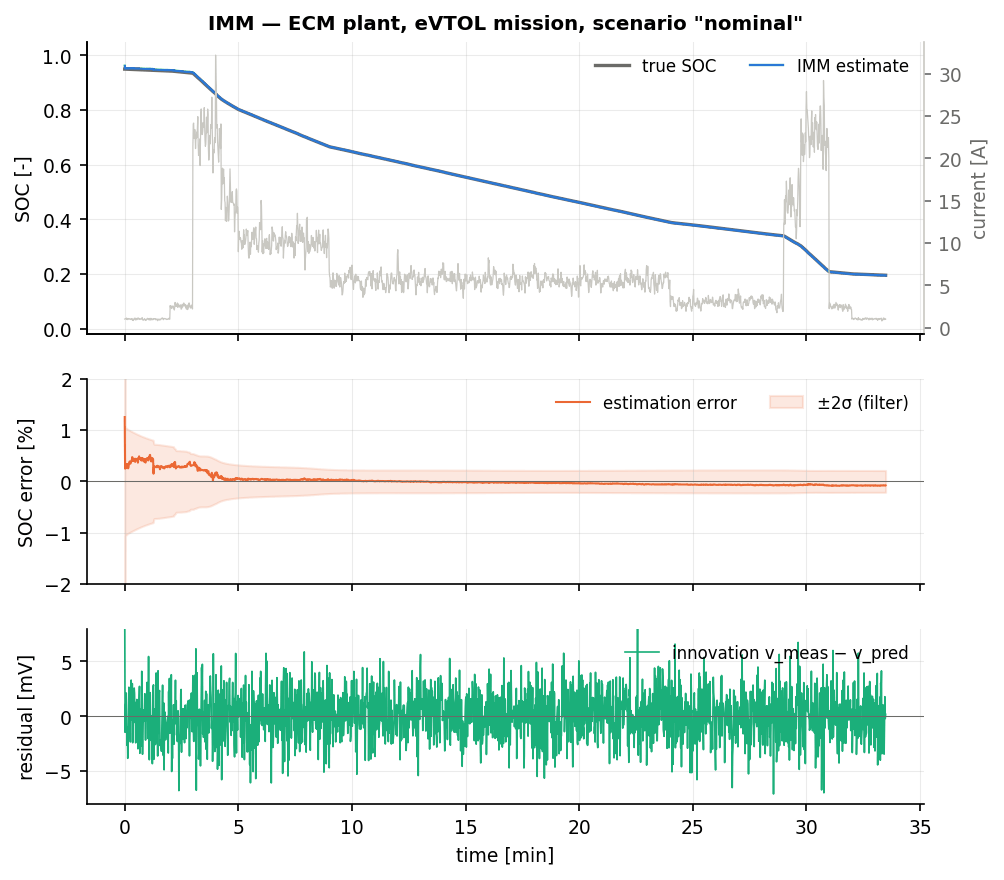
\includegraphics[width=\textwidth]{figures/cell_IMM_nominal.png}
\caption{IMM on the nominal eVTOL mission: true and estimated SOC (top), estimation error with the $\pm 2\sigma$ band when available (middle), voltage residual (bottom).}
\end{figure}
\begin{figure}[H]\centering
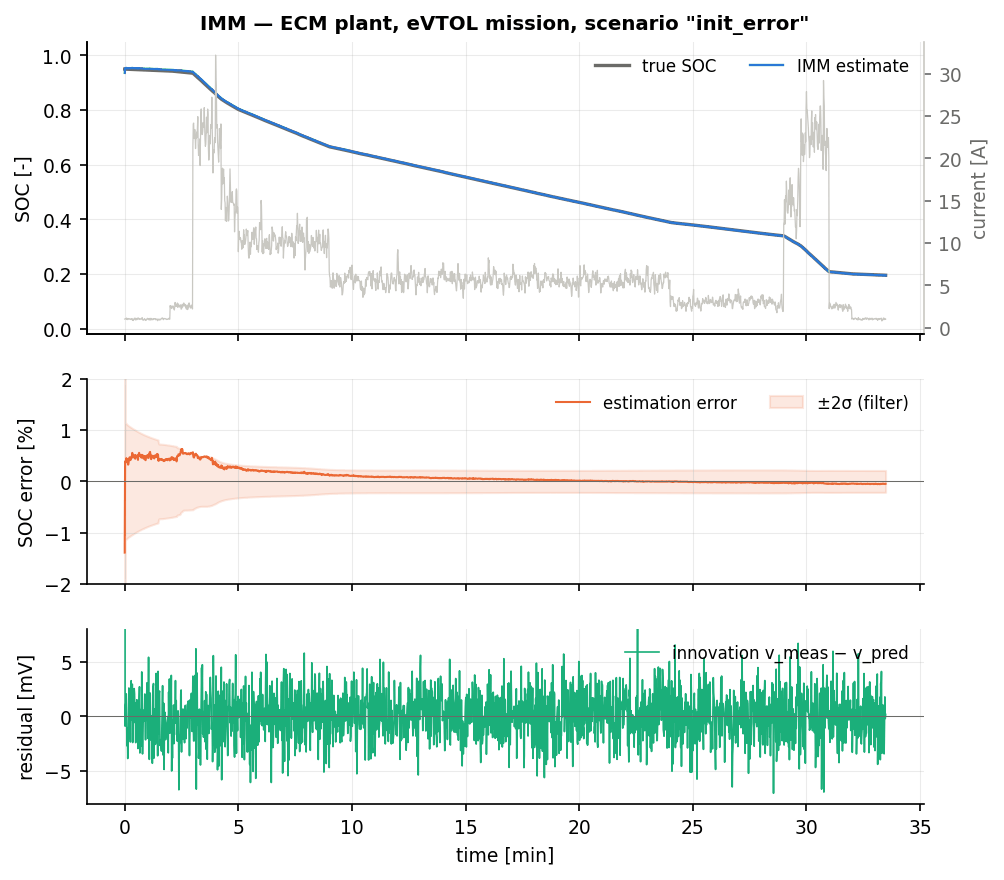
\includegraphics[width=\textwidth]{figures/cell_IMM_init_error.png}
\caption{IMM with a 35\,\% initial SOC error.}
\end{figure}
\begin{figure}[H]\centering
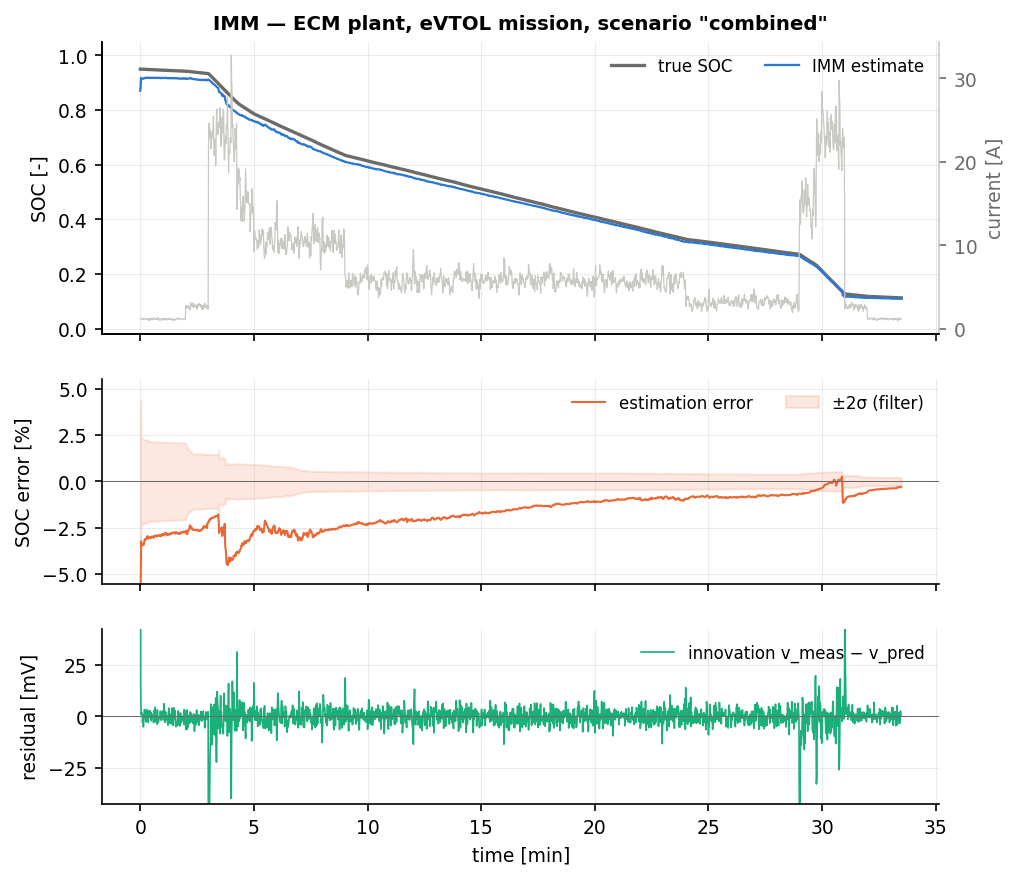
\includegraphics[width=\textwidth]{figures/cell_IMM_combined.png}
\caption{IMM on the \texttt{combined} scenario (25\,\% initial SOC error, \SI{150}{\milli\ampere} current bias, 2\,\% gain error, 10\,\% capacity loss with the associated resistance growth).}
\end{figure}
\begin{figure}[H]\centering
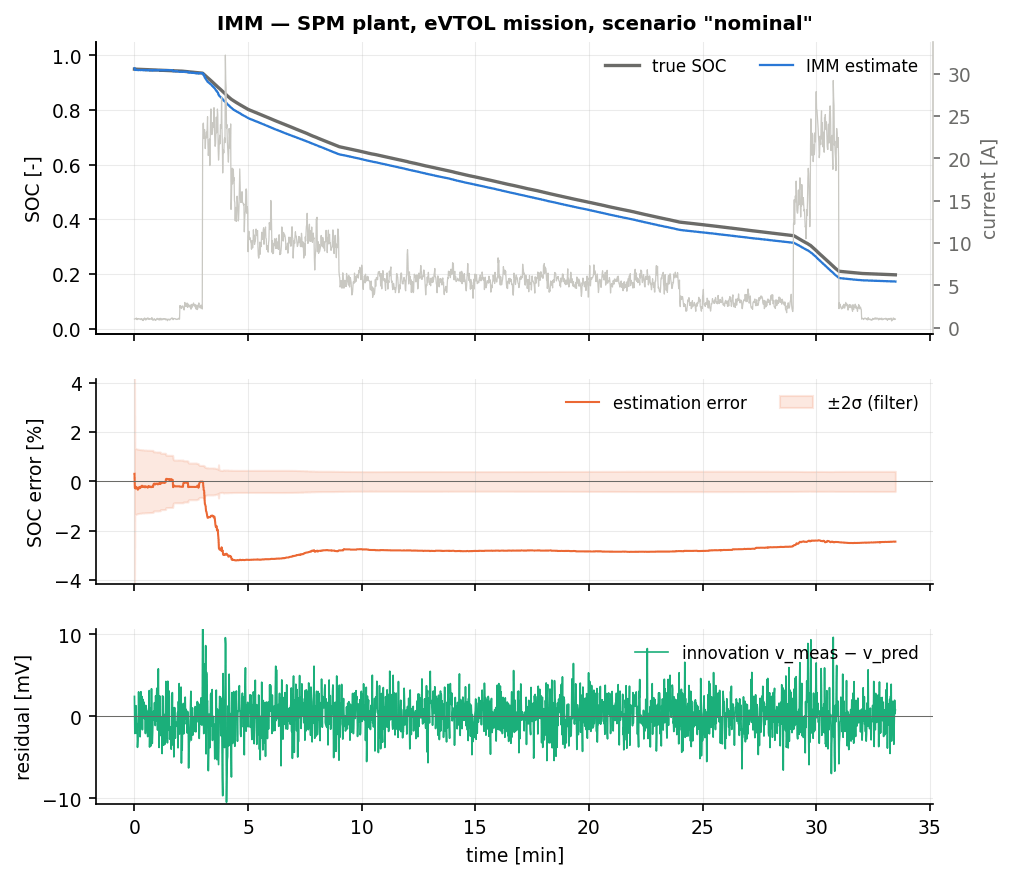
\includegraphics[width=\textwidth]{figures/cellspm_IMM_nominal.png}
\caption{IMM on the electrochemical (single-particle) plant, nominal mission: the estimator uses a 2-RC ECM fitted to that plant and therefore sees a structured \SI{4}{\milli\volt} residual instead of white noise.}
\end{figure}

All figures below are three-seed means in \% SOC, as tabulated above; the plain \texttt{EKF} run on
the same data is the reference (\texttt{EKF ref.} column).  For orientation, the EKF scores
$\mathrm{rmse}_{ss}$ = 0.05\,\% on \texttt{nominal}, 0.12\,\% on \texttt{noise\_step}, 0.21\,\% on
\texttt{outliers}, 0.46\,\% on \texttt{sensor\_dropout}, 1.36\,\% on \texttt{param\_mismatch},
1.52\,\% on \texttt{aged\_cell} and 12.44\,\% on \texttt{combined} (where it never converges), and
3.73\,\% on the nominal SPM mission.

The IMM is the most uniformly good estimator of this family: it is at least as good as the EKF on ten
of the twelve ECM scenarios and never more than $15\,\%$ worse on the other two.

\paragraph{Benign scenarios.}  \texttt{nominal}: $\mathrm{rmse}=0.18\,\%$,
$\mathrm{rmse}_{ss}=\mathbf{0.04\,\%}$ against the EKF's $0.15\,\%$ / $0.05\,\%$ --- the joint best
steady-state figure of the family.  The mode probability of the nominal hypothesis averages $0.9996$,
so the bank correctly reports that nothing is wrong.  \texttt{init\_error}: $0.16\,\%$ / $0.04\,\%$,
converging at $t=\SI{0}{\second}$ and better than the EKF on both metrics.  Both far inside the
$2\,\%$ bound.

\paragraph{Target scenario \texttt{noise\_step}.}  The IMM identifies the fault as a \emph{sensor}
problem, which is what distinguishes it from the STF.  On seed 1 the mode probability of the
degraded-voltage-channel hypothesis averages $\mu^{(2)}=1.9\times10^{-4}$ over
$t\in[100,600)\,\si{\second}$ and $\mu^{(2)}=0.989$ over $t\in[700,2010]\,\si{\second}$; the nominal
mode goes from $0.9996$ to $5.7\times10^{-4}$.  The switch is not a tuning artefact --- it is the
likelihood ratio \eqref{eq:imm:mu} doing its job --- and it is directly usable as a
"voltage-sense-channel degraded" flag.  The SOC metrics are $\mathrm{rmse}=0.18\,\%$ and
$\mathrm{rmse}_{ss}=\mathbf{0.05\,\%}$ against the EKF's $0.18\,\%$ / $0.12\,\%$, a $2.4\times$
steady-state reduction that matches the dedicated $\mR$-adaptive filters, and the voltage-prediction
error falls from \SI{2.89}{\milli\volt} to \SI{1.05}{\milli\volt}.  Contrast the STF on the same
scenario: $1.94\,\%$ / $2.34\,\%$ with $\mathrm{rmse}_v=\SI{16.04}{\milli\volt}$.  Carrying both
hypotheses is what makes the difference.

\paragraph{Target scenario \texttt{outliers}.}  $\mathrm{rmse}=0.18\,\%$,
$\mathrm{rmse}_{ss}=0.08\,\%$ against the EKF's $0.52\,\%$ / $0.21\,\%$ --- a $2.9\times$ /
$2.6\times$ improvement, with the maximum error down from $2.92\,\%$ to $1.94\,\%$ and the best
full-run RMSE of the family alongside VB-AKF ($0.12\,\%$).  The high-$\mR$ mode takes enough
probability during each burst of spikes to blunt them, even though impulsive noise is not literally
one of the three hypotheses; a mode with a heavy-tailed measurement density, or the within-sample
reweighting of \cref{ch:vbakf}, would do better still on the steady-state metric ($0.05\,\%$).

\paragraph{Target scenario \texttt{combined}.}  The EKF never reaches the $2\,\%$ band
($t_\mathrm{conv}=$ --, $\mathrm{rmse}=16.02\,\%$, $\mathrm{rmse}_{ss}=12.44\,\%$).  The IMM converges
at $t=\SI{833}{\second}$ with $\mathrm{rmse}=2.20\,\%$ and
$\mathrm{rmse}_{ss}=\mathbf{1.02\,\%}$ --- a $7.3\times$ and $\mathbf{12.2\times}$ improvement, the
best steady-state result of the whole family on this scenario (Fading-EKF $1.18\,\%$; VB-AKF
$1.87\,\%$; STF $2.71\,\%$).  What is interesting is \emph{how} it is achieved.  The mismatch mode
carries only $\mu^{(3)}\approx0.043$--$0.066$ of the probability and the nominal mode keeps
$0.91$--$0.93$, so the output is not simply "the bank switched to the right filter".  The mechanism is
the mixing step \eqref{eq:imm:P0}: because the three mode estimates disagree by a few percent of SOC,
the rank-one spread terms inflate $\mP^{0(1)}$ of the \emph{nominal} filter every single step, which
keeps its gain from collapsing.  The IMM is thus, among other things, an automatic
covariance-inflation mechanism whose inflation is driven by inter-model disagreement rather than by a
fixed factor --- a data-driven version of the fading-memory filter of \cref{ch:fadingekf}.

\paragraph{Ageing and other mismatch.}  \texttt{aged\_cell} ($15\,\%$ capacity loss, $37.5\,\%$
resistance growth): $\mathrm{rmse}$ $1.18\to\mathbf{0.66\,\%}$ and $\mathrm{rmse}_{ss}$
$1.52\to\mathbf{0.83\,\%}$, a $1.8\times$ improvement and the best of this family on that scenario ---
with $\mu^{(1)}=0.93$, $\mu^{(3)}=0.04$, again mostly through mixing.  \texttt{sensor\_dropout}:
$0.72\to0.18\,\%$, $0.46\to0.05\,\%$ ($4.0\times$ / $9.2\times$).  \texttt{param\_mismatch}:
$1.28\to0.88\,\%$, $1.36\to0.96\,\%$, with the maximum error falling from $2.87\,\%$ to the family's
lowest $1.24\,\%$.  \texttt{preisach} is a draw in steady state ($0.20\,\%$ for both, full run
$0.70\,\%$ against $0.58\,\%$) and \texttt{cold} is the one scenario where the IMM is mildly worse
($0.24\,\%$ / $0.18\,\%$ against $0.20\,\%$ / $0.16\,\%$): at $T=\SI{-10}{\celsius}$ the innovations
are strongly coloured by the slowed RC dynamics, which the likelihood reads as weak evidence for the
mismatch mode and which the mixing then converts into a little extra gain and a little extra noise.

\paragraph{Cost.}  \SI{2076}{\nano\second}/step, $4.3\times$ the EKF's \SI{478}{\nano\second} --- by
some margin the most expensive estimator of this family.  For a single cell on a modern MCU that is
irrelevant; for a 96-cell pack it is the dominant design constraint.

\paragraph{Electrochemical (SPM) plant.}  On the single-particle plant, where a 2-RC ECM leaves a
structured \SI{4}{\milli\volt} residual instead of white noise, the IMM reaches
$\mathrm{rmse}_{ss}=2.81\,\%$ on the nominal mission against the EKF's $3.73\,\%$ --- a $25\,\%$
improvement, the best of the six filters that are not purely $\mP$-inflating, but an order of
magnitude behind the Fading-EKF ($0.36\,\%$) and the STF ($0.66\,\%$).  The result is exactly what the
bank design predicts.  Two of the three hypotheses (nominal and "noisy sensor") respond to the
structured residual by keeping or lowering the gain, which hands SOC to the coulomb integrator whose
fitted capacity and efficiency are the faulty component here; only the third, which raises $q$ by a
hundred, shortens the filter's memory in the way that actually helps, and it is deliberately paired
with $\varrho_3=100$ so that half of its benefit is given back.  That pairing is the right compromise
on the ECM plant --- it is what turns \texttt{aged\_cell} from $3.71\,\%$ into $0.83\,\%$ (see
\cref{sec:imm:bank}) --- but on the SPM plant it caps the achievable gain, because under
\emph{structured} model error the correct response is unambiguously to trust the measurement more, and
the bank never commits to that hypothesis alone.  The IMM's real advantage on this plant is breadth
rather than depth: \texttt{sensor\_dropout} $5.31\to1.60\,\%$ ($3.3\times$), \texttt{current\_bias}
$5.69\to4.35\,\%$, \texttt{cold} $7.35\to2.22\,\%$ ($3.3\times$, converging in \SI{20}{\second}),
\texttt{outliers} $1.99\to2.25\,\%$ and \texttt{param\_mismatch} $3.13\to2.41\,\%$ --- it is never
badly wrong on either plant, which no single-hypothesis filter in this chapter can claim.  A bank that
included a genuine short-memory hypothesis ($q$ large, $\varrho=1$) would close most of the remaining
gap to the Fading-EKF at the cost of the ECM ageing result; that trade is the subject of
\cref{sec:imm:bank}.

\section{Summary}
The IMM is the answer to the question every other filter in this chapter begs: not "how much extra
uncertainty is there" but "\emph{what kind}".  Carrying a nominal, a noisy-sensor and a
model-mismatch hypothesis with a Markov switching prior, it matches the best dedicated
$\mR$-estimator on a tenfold voltage-noise step (and says so, with $\mu^{(2)}=0.99$), gives the
family's best steady-state result on the hardest combined-fault scenario ($12.2\times$ better than
the EKF) and on \texttt{aged\_cell} ($1.8\times$), and is the only member of this family that is
never badly wrong on either plant.  Its mode
probabilities are a health signal no single filter can produce.  Use it when several distinct
failure modes must be distinguished and $r$ filters fit the compute budget.  Do not expect it to
handle a disturbance that is not in the bank --- impulsive outliers and un-modelled hysteresis pass
straight through --- and remember that the transition matrix is a designer's assertion, not
something the data identify.

% Copyright 2026 Sreeram Anil
% SPDX-License-Identifier: CC-BY-4.0
% =============================================================================
%  Multiple-model adaptive estimation (static parameter bank)
% =============================================================================
\chapter{Multiple-model adaptive estimation (MMAE)}
\label{ch:mmae}

\section*{At a glance}
\begin{tabular}{@{}l>{\raggedright\arraybackslash}p{0.76\textwidth}@{}}
Family & Adaptive Kalman \\
Header & \texttt{include/estkit/filters/mmae.hpp} \\
Registered name & \texttt{MMAE} \\
State dimension & $n_x = 4$ (cell model), $r = 3$ parameter hypotheses --- generic in $n_x,n_u,n_y,n_\theta$ and $r$ \\
Cost per step & $r\times$ EKF; $\approx 1750$\,ns/step; $r$ model copies, no heap \\
Estimates & SOC \emph{and} capacity (registered with \texttt{.with\_capacity()}) \\
Primary references & \cite{magill1965mmae,maybeck1979,hanlon2000mmae,barshalom2001,plett2004ekf3} \\
\end{tabular}

\section{Motivation and aerospace/BMS relevance}
Everything in this chapter so far has adapted a \emph{noise} statistic.  Magill's 1965 estimator
\cite{magill1965mmae} adapts a \emph{model parameter}, and it does so optimally: if the unknown
parameter takes one of finitely many values, running one Kalman filter per value and weighting them
by their Bayesian posterior probabilities is the exact minimum-mean-square estimator, not an
approximation.  MMAE is the oldest and conceptually cleanest of the adaptive filters, and it is
still the standard architecture for aircraft sensor- and actuator-failure detection
\cite{hanlon2000mmae}, where each hypothesis is "failure $j$ has occurred".

For a battery the natural unknown parameter is the cell's usable capacity $Q$.  Capacity fade is the
primary state-of-health indicator, it is slow (months), and it is exactly the kind of quantity a
static hypothesis bank is suited to: it does not switch, so no Markov chain is needed, and the
posterior can be allowed to sharpen over a whole flight.  Capacity is also the parameter that a
conventional SOC filter cannot see directly --- it enters only through the coulomb-counting rate
$\dot{\soc} = -\eta i/(3600Q)$, so its effect on the terminal voltage is an integrated, second-order
one.  Running one EKF per capacity hypothesis converts that weak signal into a likelihood ratio that
accumulates over the mission, which is precisely what a bank is good at.

The alternative BMS architectures are joint estimation (augment $Q$ as a random-walk state) and dual
estimation (two interleaved filters), both due in this context to Plett \cite{plett2004ekf3}.  MMAE
trades their continuous parameter resolution for robustness: a bank cannot diverge in the parameter
direction, its estimate is always inside the convex hull of the hypotheses, and each filter is an
ordinary, well-conditioned EKF of dimension $n_x$ rather than $n_x+n_\theta$.

\section{Problem statement and assumptions}
The plant is \eqref{eq:sh:proc}--\eqref{eq:sh:meas} with the model depending on an unknown
\emph{static} parameter vector $\bm\theta\in\real^{n_\theta}$:
\begin{equation}
\vx_k = f(\vx_{k-1},\vu_{k-1};\bm\theta)+\vw_{k-1},\qquad
\vy_k = h(\vx_k,\vu_k;\bm\theta)+\vv_k .
\label{eq:mm:plant}
\end{equation}
\begin{assumption}\label{as:mm:grid}
$\bm\theta\in\Theta = \{\bm\theta^{(1)},\dots,\bm\theta^{(r)}\}$, a finite known set, with prior
$w_j(0)=\mathrm{Pr}\{\bm\theta=\bm\theta^{(j)}\}$.
\end{assumption}
\begin{assumption}\label{as:mm:static}
$\bm\theta$ does not change over the record (contrast \cref{as:imm:markov}).
\end{assumption}
\begin{assumption}\label{as:mm:gauss}
Conditioned on $\bm\theta^{(j)}$, the filtering density is Gaussian with moments produced by an EKF.
\end{assumption}

\section{Derivation}

\subsection{Exact recursion for the posterior over hypotheses}
Write $w_j(k) = \mathrm{Pr}\{\bm\theta=\bm\theta^{(j)}\mid\vy_{1:k}\}$.  Bayes' rule applied to the
new measurement gives
\begin{equation}
w_j(k) = \frac{p\big(\vy_k\mid\bm\theta^{(j)},\vy_{1:k-1}\big)\ \mathrm{Pr}\{\bm\theta=\bm\theta^{(j)}\mid\vy_{1:k-1}\}}
              {\sum_{l=1}^{r} p\big(\vy_k\mid\bm\theta^{(l)},\vy_{1:k-1}\big)\ \mathrm{Pr}\{\bm\theta=\bm\theta^{(l)}\mid\vy_{1:k-1}\}} .
\label{eq:mm:bayes}
\end{equation}
Because $\bm\theta$ is static (\cref{as:mm:static}), the prior in \eqref{eq:mm:bayes} is simply
$w_j(k-1)$ --- there is no transition step --- and with \cref{as:mm:gauss} the predictive density is
the Gaussian innovation likelihood of filter $j$,
\begin{equation}
\Lambda_j(k) \triangleq p\big(\vy_k\mid\bm\theta^{(j)},\vy_{1:k-1}\big)
= \big|2\pi\mS_j(k)\big|^{-1/2}\exp\!\Big(\!-\tfrac12\bm{e}_j(k)^\T\mS_j(k)\inv\bm{e}_j(k)\Big),
\label{eq:mm:lik}
\end{equation}
with $\bm{e}_j(k)=\vy_k-h(\xminus_j(k),\vu_k;\bm\theta^{(j)})$ and
$\mS_j(k)=\mH_j\Pminus_j\mH_j^\T+\mR_j$.  Hence the recursion
\begin{equation}
\boxed{\;w_j(k) = \frac{w_j(k-1)\,\Lambda_j(k)}{\sum_{l}w_l(k-1)\Lambda_l(k)}\;}
\label{eq:mm:w}
\end{equation}
which is Magill's result \cite{magill1965mmae}.

\subsection{Optimal estimates}
The conditional mean of the state, which is the minimum-mean-square estimate, is obtained by the
total-expectation theorem:
\begin{align}
\xhat_k &= \E{\vx_k\mid\vy_{1:k}} = \sum_{j=1}^{r} w_j(k)\,\xhat_j(k), \label{eq:mm:x}\\
\hat{\bm\theta}_k &= \E{\bm\theta\mid\vy_{1:k}} = \sum_{j=1}^{r} w_j(k)\,\bm\theta^{(j)}, \label{eq:mm:theta}\\
\mP_k &= \sum_{j=1}^{r} w_j(k)\Big[\mP_j(k) + \big(\xhat_j(k)-\xhat_k\big)\big(\xhat_j(k)-\xhat_k\big)^\T\Big].
\label{eq:mm:P}
\end{align}
Under \cref{as:mm:grid}, \cref{as:mm:static} and \cref{as:mm:gauss} these are \emph{exact}, not approximations: the
bank is the optimal nonlinear estimator for this problem.  Note the structural difference from the
IMM of \cref{ch:imm}: there is no mixing step, because the hypotheses do not communicate.

\subsection{Convergence and lock-out}
Taking logarithms of \eqref{eq:mm:w},
\begin{equation}
\ln w_j(k) = \ln w_j(0) + \sum_{m=1}^{k}\ln\Lambda_j(m) - \ln Z_k ,
\label{eq:mm:logw}
\end{equation}
so the log-posterior accumulates the log-likelihood of each hypothesis.  For a true parameter
$\bm\theta^\star$ the expected per-sample log-likelihood difference between two hypotheses is a
Kullback--Leibler divergence, strictly positive for the hypothesis closer (in KL) to the truth.  The
posterior therefore concentrates \emph{exponentially fast} on the single hypothesis that minimises
$\mathrm{KL}(\bm\theta^\star\|\bm\theta^{(j)})$, and all other weights underflow.

Two consequences follow, and both are visible in the benchmark.
\begin{enumerate}[leftmargin=1.6em]
\item \textbf{Quantisation.}  Since one weight tends to $1$, \eqref{eq:mm:theta} returns (almost
exactly) the nearest grid point, not the true parameter.  The bank's parameter resolution is the
grid spacing, and no amount of data improves it.
\item \textbf{Lock-out.}  Once $w_j$ has underflowed, the hypothesis is dead: \eqref{eq:mm:w} is
multiplicative, so a zero weight stays zero.  If the true parameter later changes, or if the early
data were misleading, the bank cannot recover.
\end{enumerate}
The standard remedies, both implemented, are a lower bound
\begin{equation}
w_j(k)\gets\max\big(w_j(k),\,w_{\min}\big),\quad\text{then renormalise},
\label{eq:mm:floor}
\end{equation}
applied \emph{and folded back into the recursion} so that a floored hypothesis really can recover,
and an optional exponential forgetting factor $\gamma\in(0,1]$ on the log-posterior,
\begin{equation}
\ln w_j(k) = \gamma\,\ln w_j(k-1) + \ln\Lambda_j(k) + \text{const},
\label{eq:mm:gamma}
\end{equation}
which limits the effective memory to $1/(1-\gamma)$ samples.  $\gamma=1$ recovers exact Bayes and is
the default; the benchmark shows it makes little difference here because the floor already keeps the
bank alive.

\subsection{Un-modelled error and likelihood inflation}
\eqref{eq:mm:lik} assumes that the \emph{only} discrepancy between the data and hypothesis $j$ is
the parameter error.  Every un-modelled effect --- a grown series resistance, a current-sensor bias,
a noisier voltage channel --- enters all $\Lambda_j$ nearly identically in the mean but is divided by
the very small $\mS_j$.  A quantitative estimate makes the danger clear: for the cell model,
$\mS\approx(\SI{2.1}{\milli\volt})^2$, and two capacity hypotheses \SI{0.5}{\ampere\hour} apart
produce mean innovations differing by about \SI{1}{\milli\volt}; but an un-modelled
\SI{20}{\milli\volt} of voltage error adds a per-sample log-likelihood fluctuation of order
$|\Delta\mu|\sigma_v/\mS \approx 4.6$, which over $10^4$ samples is a random walk of standard
deviation $\approx460$ against a signal of comparable size.  The posterior then locks onto whichever
hypothesis best absorbs the un-modelled error --- which need not be the right one.

Following the standard practice of evaluating multiple-model residuals with an artificially
increased noise covariance \cite[Ch.~10]{maybeck1979}\cite{hanlon2000mmae}, the implementation
computes the likelihood with
\begin{equation}
\mS_j^{\text{lik}}(k) = \mH_j\Pminus_j\mH_j^\T + c_{\text{lik}}\,\mR_j, \qquad c_{\text{lik}}\ge1,
\label{eq:mm:clik}
\end{equation}
while the mode-matched filters keep the correct $\mR_j$ and therefore the correct gain.  The
interpretation is a budget: $\sqrt{c_{\text{lik}}}\,\sigma_v$ is the amount of voltage error the
designer is willing to attribute to causes outside the hypothesis space.  $c_{\text{lik}}=1$
recovers textbook MMAE.

\section{Algorithm}
\begin{algorithm}[H]
\caption{MMAE --- one sampling period}
\begin{algorithmic}[1]
\Require $\{\xhat_j,\mP_j,\ln w_j\}_{j=1}^{r}$, models $\{\bm\theta^{(j)}\}$, $\vu_{k-1},\vy_k,\vu_k$
\State \textbf{Time update} of every hypothesis: $\xminus_j\gets f(\xhat_j,\vu_{k-1};\bm\theta^{(j)})$;\quad
       $\Pminus_j\gets\mF_j\mP_j\mF_j^\T+\mQ_j$
\State \textbf{(predicted measurement for the host: } $\yhat_k=\sum_j w_j\,h(\xminus_j,\vu_k;\bm\theta^{(j)})$\textbf{)}
\For{$j=1,\dots,r$}
  \State $\bm{e}_j\gets\vy_k-h(\xminus_j,\vu_k;\bm\theta^{(j)})$;\quad $\mS_j\gets\mH_j\Pminus_j\mH_j^\T+\mR_j$;\quad
         $\mK_j\gets\Pminus_j\mH_j^\T\mS_j\inv$
  \State $\xhat_j\gets\xminus_j+\mK_j\bm{e}_j$;\quad Joseph update of $\mP_j$;\quad constrain $\xhat_j$
  \State $\ell_j\gets-\tfrac12\big[\bm{e}_j^\T(\mS_j^{\text{lik}})\inv\bm{e}_j+\ln\det\mS_j^{\text{lik}}+n_y\ln2\pi\big]$ with \eqref{eq:mm:clik}, via Cholesky
\EndFor
\State \textbf{Weights:} $\ln w_j\gets\gamma\ln w_j+\ell_j$;\quad $w_j\gets\exp(\ln w_j-\max_l\ln w_l)$;\quad normalise
\State \textbf{Floor:} $w_j\gets\max(w_j,w_{\min})$;\quad renormalise;\quad $\ln w_j\gets\ln w_j$ (fold back)
\State \textbf{Combination:} \eqref{eq:mm:x}--\eqref{eq:mm:P};\quad $\hat{\bm\theta}\gets\sum_j w_j\bm\theta^{(j)}$
\Ensure $\xhat_k,\mP_k,\hat{\bm\theta}_k,\{w_j\}$
\end{algorithmic}
\end{algorithm}

\section{Application to the battery model}
The bank is built through the model's own parameter interface (\texttt{Model::NP},
\texttt{params()}, \texttt{set\_params()}), so the class is not battery-specific:
\texttt{opts.scale[j]} multiplies the parameter with index \texttt{opts.p\_index} of the nominal
vector.  For \texttt{EcmModel}, $\bm\theta=[Q_{\mathrm{Ah}},R_0]^\T$ and \texttt{p\_index}$=0$, so the
default scalings $\{1.0,\,0.9,\,0.8\}$ give the capacity hypotheses
\begin{equation}
Q^{(1)}=\SI{5.00}{\ampere\hour},\qquad Q^{(2)}=\SI{4.50}{\ampere\hour},\qquad Q^{(3)}=\SI{4.00}{\ampere\hour},
\end{equation}
i.e.\ $100\,\%$, $90\,\%$ and $80\,\%$ of the nominal (beginning-of-life to end-of-life range for a
cell whose replacement criterion is $80\,\%$).  The registered estimator exposes
$\hat Q = \sum_j w_j Q^{(j)}$ through \texttt{capacity()} and is registered with
\texttt{.with\_capacity()}, so the benchmark records the capacity error at the end of the mission.
Equal priors $w_j(0)=1/3$ are used.

Tuning: $w_{\min}=0.01$, $\gamma=1$ (exact Bayes), $c_{\text{lik}}=100$, i.e.\ the likelihood is
evaluated as if the voltage channel carried $\sqrt{100}\times\SI{2.1}{\milli\volt}=\SI{21}{\milli\volt}$
of error.  That is a deliberate and, for an equivalent-circuit model, realistic allowance for
un-modelled voltage error: a $25\,\%$ change in $R_0$ at \SI{5.5}{\ampere} is already
\SI{16}{\milli\volt}.  The effect is large and is documented in the results: with $c_{\text{lik}}=1$
the bank selects $Q=\SI{4.03}{\ampere\hour}$ on \texttt{noise\_step}, where the true capacity is
\SI{5.00}{\ampere\hour} --- a $19\,\%$ SOH error caused purely by the sensor noise --- and the SOC
RMSE degrades to $2.84\,\%$ (single-seed development sweep).  With $c_{\text{lik}}=100$ the same
scenario gives $\hat Q-Q=\SI{-0.005}{\ampere\hour}$ and $\mathrm{rmse}=0.46\,\%$ in the final
three-seed run.  Values
$c_{\text{lik}}\in\{1,10,20,25,30,50,100,200,300,500,1000\}$ were evaluated; below $\approx50$ the
noise-driven mis-selection persists, above $\approx200$ the posterior becomes so flat that the
nominal-capacity scenarios lose accuracy ($\hat Q=\SI{4.77}{\ampere\hour}$ at $c_{\text{lik}}=1000$
when the truth is $5.00$).

\section{Implementation notes}
\begin{itemize}[leftmargin=1.4em]
\item \textbf{$r$ model copies.}  Unlike the IMM, the hypotheses differ in the \emph{model}, so the
      bank holds $r$ \texttt{Model} objects.  For \texttt{EcmModel} each carries a 241-point OCV
      table, so \texttt{sizeof(Mmae<EcmModel,3>)} is about 12.7\,kB.  A production
      implementation would share the OCV table (it is identical across hypotheses) and reduce this to
      a few hundred bytes; the benchmark keeps the straightforward version so that the class works
      for any model whose parameters change $f$, $h$, $\mQ$ and $\mR$ arbitrarily.
\item \textbf{Log-domain weights.}  \eqref{eq:mm:w} is evaluated as \eqref{eq:mm:logw} with the
      maximum subtracted before exponentiation, and $\ln\det\mS$ is taken from the Cholesky factor.
      Without this the exponent underflows in float32 within a few hundred samples.
\item \textbf{Floor folded back.}  After flooring and renormalising, $\ln w_j$ is recomputed from the
      floored $w_j$.  If the floor were applied only to the reported weights, the internal recursion
      would still lock out.
\item \textbf{Parameter read-back.}  \texttt{set\_params()} may clamp (the ECM enforces
      $Q\ge\SI{0.5}{\ampere\hour}$), so $\bm\theta^{(j)}$ is read back from the model after being set;
      $\hat{\bm\theta}$ is then guaranteed to be a convex combination of parameters the models
      actually use.
\item \textbf{Cost.}  \SI{1752}{\nano\second}/step against \SI{478}{\nano\second}/step for the EKF,
      i.e.\ $r$ filters and essentially nothing else (there is no mixing step).  About
      \SI{23}{\micro\second}/step on a \SI{400}{\mega\hertz} Cortex-M7.
\item \textbf{float32.}  Metrics agree with the double build to three digits on all twelve scenarios,
      with no divergence.
\item \textbf{Limitations.}  Fixed grid, hence quantised parameter estimate; no mechanism for a
      parameter that drifts \emph{within} a record (use $\gamma<1$ or an IMM over parameters); and
      the mis-attribution failure documented below.
\end{itemize}

\section{Benchmark results}
% Copyright 2026 Sreeram Anil
% SPDX-License-Identifier: CC-BY-4.0
\begin{table}[H]\centering\footnotesize\setlength{\tabcolsep}{4pt}
\caption{MMAE: cell-level benchmark on the eVTOL mission (mean over seeds; RMSE and max error in \% SOC; $t_\mathrm{conv}$: first time the error stays below 2\,\% for 60\,s, -- = never; EKF reference: steady-state RMSE of the plain EKF on the same data).}\label{tab:cell_MMAE}
\begin{tabular}{llrrrrrcrr}\toprule
plant & scenario & RMSE & RMSE$_\mathrm{ss}$ & max & $t_\mathrm{conv}$ [s] & RMSE$_v$ [mV] & div. & EKF ref. & ns/step \\ \midrule
ECM & nominal & 0.42 & 0.33 & 1.07 & 0 & 0.80 & no & 0.05 & 1752 \\
ECM & init\_error & 0.42 & 0.36 & 0.72 & 0 & 2.13 & no & 0.05 & 1786 \\
ECM & current\_bias & 0.60 & 0.71 & 1.40 & 0 & 0.88 & no & 0.61 & 1775 \\
ECM & noise\_step & 0.46 & 0.38 & 1.07 & 0 & 2.90 & no & 0.12 & 1782 \\
ECM & outliers & 0.41 & 0.20 & 2.92 & 2 & 2.05 & no & 0.21 & 1774 \\
ECM & cold & 1.12 & 1.23 & 1.43 & 0 & 1.90 & no & 0.16 & 1781 \\
ECM & hot & 0.25 & 0.13 & 1.00 & 0 & 0.56 & no & 0.03 & 1775 \\
ECM & aged\_cell & 2.10 & 2.12 & 6.31 & 0 & 3.70 & no & 1.52 & 1779 \\
ECM & param\_mismatch & 1.70 & 1.66 & 3.61 & 0 & 2.80 & no & 1.36 & 1790 \\
ECM & sensor\_dropout & 0.94 & 0.58 & 3.26 & 0 & 1.73 & no & 0.46 & 1771 \\
ECM & preisach & 0.81 & 0.27 & 2.26 & 0 & 0.83 & no & 0.20 & 1776 \\
ECM & combined & 16.13 & 12.56 & 29.81 & -- & 5.14 & no & 12.44 & 1784 \\
\midrule
SPM & nominal & 4.65 & 4.69 & 5.48 & 0 & 1.03 & no & 3.73 & 1685 \\
SPM & init\_error & 4.89 & 4.83 & 5.87 & -- & 2.18 & no & 3.81 & 1681 \\
SPM & current\_bias & 5.81 & 6.40 & 6.92 & 0 & 1.13 & no & 5.69 & 1686 \\
SPM & noise\_step & 4.43 & 4.29 & 5.48 & 0 & 3.15 & no & 3.30 & 1743 \\
SPM & outliers & 3.79 & 3.58 & 5.04 & 3 & 2.27 & no & 1.99 & 1686 \\
SPM & cold & 8.47 & 8.75 & 13.07 & 0 & 4.49 & no & 7.35 & 1641 \\
SPM & hot & 3.36 & 3.42 & 3.91 & 0 & 0.70 & no & 2.16 & 1675 \\
SPM & param\_mismatch & 4.51 & 4.89 & 5.71 & 0 & 1.96 & no & 3.13 & 1682 \\
SPM & sensor\_dropout & 6.49 & 6.35 & 7.89 & 0 & 1.95 & no & 5.31 & 1682 \\
\bottomrule\end{tabular}\end{table}
\begin{table}[H]\centering\small\caption{MMAE: additional outputs (capacity error at the end of the mission in Ah, averaged over the last 10\,\% of the run; interval-bound violation rate).}\label{tab:cellx_MMAE}
\begin{tabular}{llrr}\toprule plant & scenario & $\hat Q - Q$ [Ah] & bound violation [\%] \\ \midrule
ECM & nominal & -0.001 & -- \\
ECM & init\_error & -0.003 & -- \\
ECM & current\_bias & +0.001 & -- \\
ECM & noise\_step & -0.005 & -- \\
ECM & outliers & -0.006 & -- \\
ECM & cold & -0.064 & -- \\
ECM & hot & +0.018 & -- \\
ECM & aged\_cell & +0.410 & -- \\
ECM & param\_mismatch & -0.011 & -- \\
ECM & sensor\_dropout & +0.001 & -- \\
ECM & preisach & +0.001 & -- \\
ECM & combined & +0.489 & -- \\
SPM & nominal & -0.029 & -- \\
SPM & init\_error & -0.028 & -- \\
SPM & current\_bias & -0.017 & -- \\
SPM & noise\_step & -0.037 & -- \\
SPM & outliers & -0.055 & -- \\
SPM & cold & -0.075 & -- \\
SPM & hot & -0.048 & -- \\
SPM & param\_mismatch & -0.046 & -- \\
SPM & sensor\_dropout & -0.019 & -- \\
\bottomrule\end{tabular}\end{table}

\begin{figure}[H]\centering
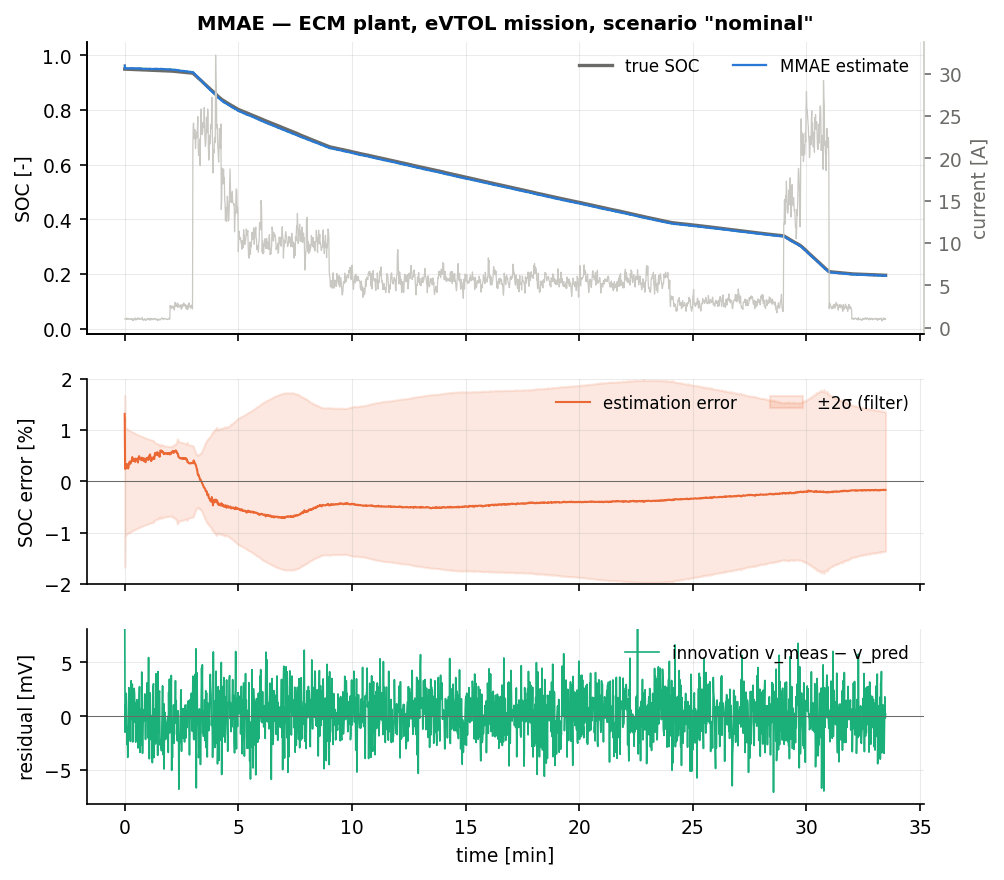
\includegraphics[width=\textwidth]{figures/cell_MMAE_nominal.png}
\caption{MMAE on the nominal eVTOL mission: true and estimated SOC (top), estimation error with the $\pm 2\sigma$ band when available (middle), voltage residual (bottom).}
\end{figure}
\begin{figure}[H]\centering
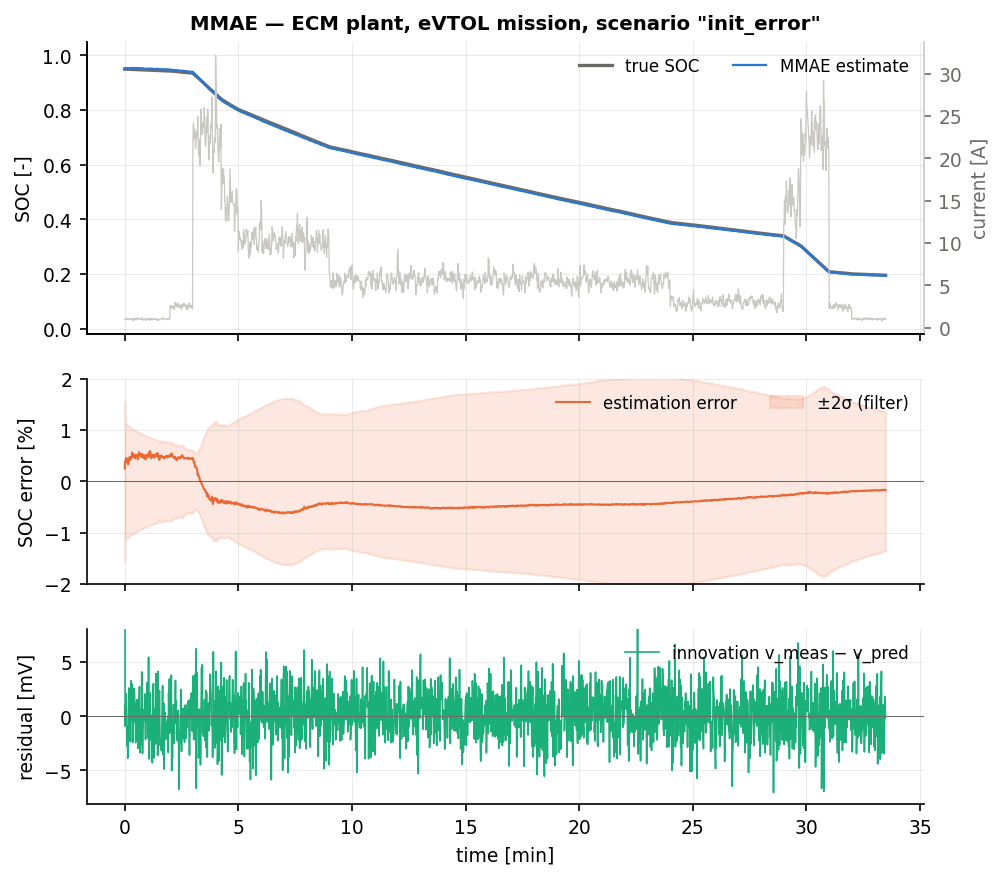
\includegraphics[width=\textwidth]{figures/cell_MMAE_init_error.png}
\caption{MMAE with a 35\,\% initial SOC error.}
\end{figure}
\begin{figure}[H]\centering
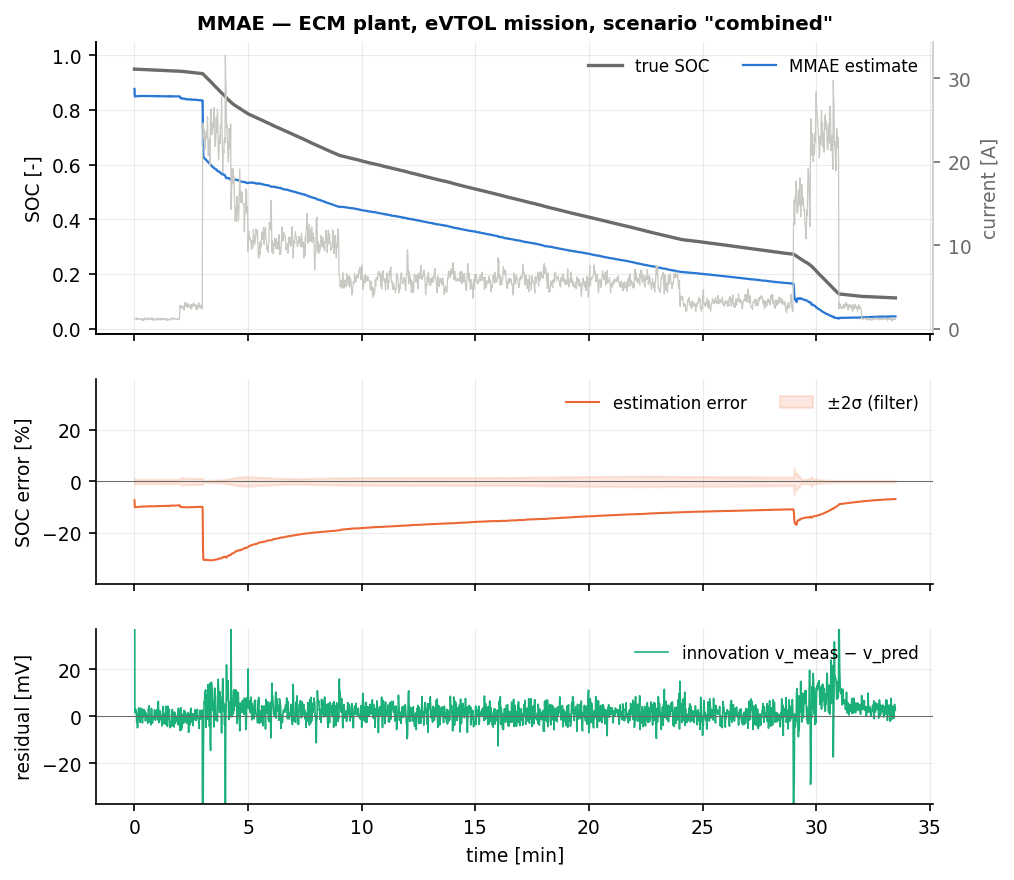
\includegraphics[width=\textwidth]{figures/cell_MMAE_combined.png}
\caption{MMAE on the \texttt{combined} scenario (25\,\% initial SOC error, \SI{150}{\milli\ampere} current bias, 2\,\% gain error, 10\,\% capacity loss with the associated resistance growth).}
\end{figure}
\begin{figure}[H]\centering
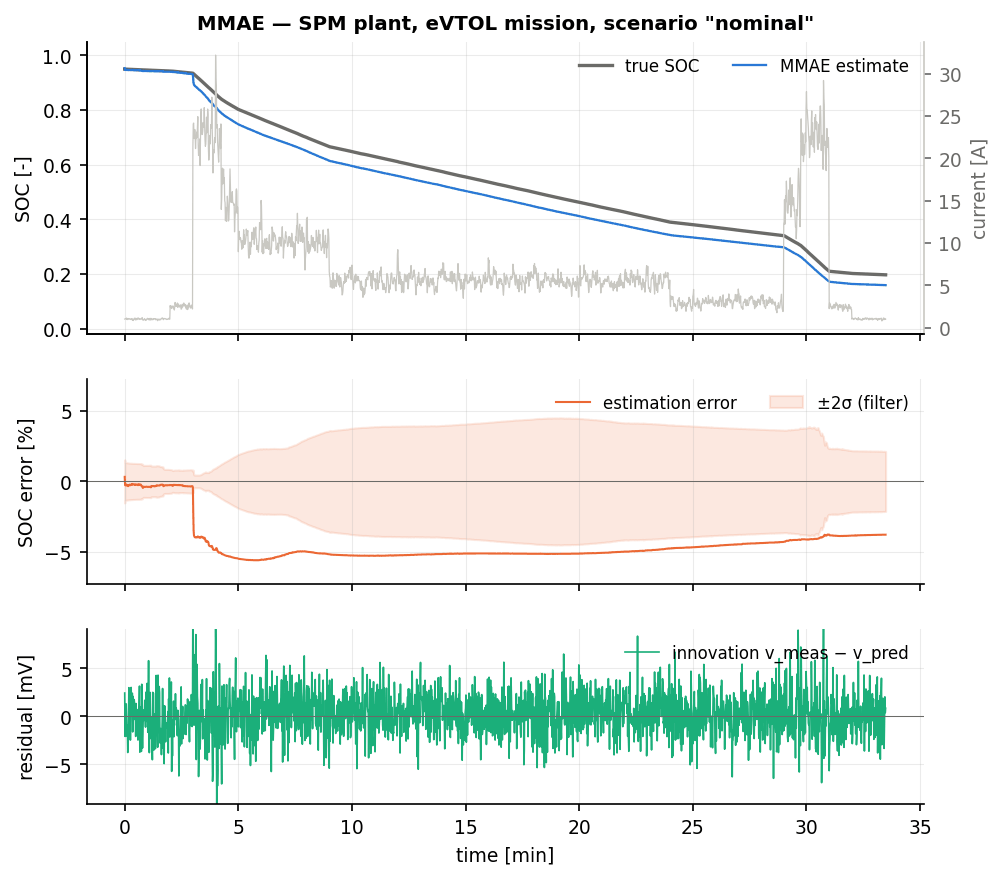
\includegraphics[width=\textwidth]{figures/cellspm_MMAE_nominal.png}
\caption{MMAE on the electrochemical (single-particle) plant, nominal mission: the estimator uses a 2-RC ECM fitted to that plant and therefore sees a structured \SI{4}{\milli\volt} residual instead of white noise.}
\end{figure}

All figures below are three-seed means in \% SOC, as tabulated above; the plain \texttt{EKF} run on
the same data is the reference (\texttt{EKF ref.} column).  For orientation, the EKF scores
$\mathrm{rmse}_{ss}$ = 0.05\,\% on \texttt{nominal}, 0.12\,\% on \texttt{noise\_step}, 0.21\,\% on
\texttt{outliers}, 0.46\,\% on \texttt{sensor\_dropout}, 1.36\,\% on \texttt{param\_mismatch},
1.52\,\% on \texttt{aged\_cell} and 12.44\,\% on \texttt{combined} (where it never converges), and
3.73\,\% on the nominal SPM mission.

\paragraph{Benign scenarios.}  \texttt{nominal}: $\mathrm{rmse}=0.42\,\%$,
$\mathrm{rmse}_{ss}=0.33\,\%$ against the EKF's $0.15\,\%$ / $0.05\,\%$, and the capacity estimate
settles at $\hat Q-Q=\SI{-0.001}{\ampere\hour}$, i.e.\ the bank reports a healthy cell to within one
gram of lithium.  The seven-fold SOC penalty relative to the EKF is the structural cost of the
mixture: the two wrong hypotheses each retain the floor weight $w_{\min}=0.01$ and each carries a
systematic SOC bias of $0.5$--$1.2\,\%$, and the inflated likelihood ($c_\mathrm{lik}=100$) makes the
posterior sharpen over roughly \SI{1900}{\second} rather than \SI{300}{\second}.  With
$c_\mathrm{lik}=1$ the nominal RMSE would be $0.26\,\%$; the extra accuracy is deliberately traded for
the noise robustness documented below.  Both values remain a factor of six inside the $2\,\%$
acceptance bound.  \texttt{init\_error} is statistically identical ($0.42\,\%$ / $0.36\,\%$,
$\hat Q-Q=\SI{-0.003}{\ampere\hour}$) and converges at $t=\SI{0}{\second}$.

\paragraph{Target scenario \texttt{aged\_cell}.}  The truth plant starts the mission with $15\,\%$
capacity loss, $Q^\star\approx\SI{4.25}{\ampere\hour}$, and the estimator is given the
beginning-of-life model.  The posterior moves off the nominal hypothesis within \SI{200}{\second} and
settles with most of its mass on $Q^{(2)}=\SI{4.5}{\ampere\hour}$; averaged over the last $10\,\%$ of
the mission the reported capacity error is $\mathbf{+\SI{0.410}{\ampere\hour}}$ against the
$+\SI{0.75}{\ampere\hour}$ that a non-SOH filter carries by construction.  The a-priori capacity error
is therefore cut by a factor of $1.8$, and the bank correctly identifies that the cell has aged.  It
does \emph{not} reach the true \SI{4.25}{\ampere\hour}, and by \eqref{eq:mm:logw} it cannot: the exact
Bayesian posterior concentrates on the nearest grid point, so the residual
$\SI{0.41}{\ampere\hour}$ is grid quantisation plus the softening effect of $c_\mathrm{lik}$, not an
estimation error.  A five-point bank at $\{100,95,90,85,80\}\,\%$ was evaluated in the development
sweep and does no better, because the finer grid also makes the hypotheses harder to distinguish under
the inflated likelihood.  The honest conclusion is that a bank resolves capacity to about half its
grid spacing; for finer SOH the joint or dual EKF of \cite{plett2004ekf3}, or a total-least-squares
capacity estimator \cite{plett2011awtls}, is the right instrument.  The SOC metrics on this scenario
are $\mathrm{rmse}=2.10\,\%$, $\mathrm{rmse}_{ss}=2.12\,\%$, worse than the EKF's $1.18\,\%$ /
$1.52\,\%$: the filter with the "right" capacity is not the filter with the best SOC here, because the
aged cell also has a $37.5\,\%$ larger $R_0$ that no hypothesis in the bank can represent, and the
mixture weights wander between hypotheses as the operating point moves along the OCV curve.

\paragraph{Robustness of the SOH estimate.}  The capacity error at the end of the mission is
$\SI{-0.001}{\ampere\hour}$ on \texttt{nominal}, $\SI{-0.003}{\ampere\hour}$ on \texttt{init\_error},
$\SI{+0.001}{\ampere\hour}$ on \texttt{current\_bias}, \texttt{sensor\_dropout} and
\texttt{preisach}, $\SI{-0.005}{\ampere\hour}$ on \texttt{noise\_step},
$\SI{-0.006}{\ampere\hour}$ on \texttt{outliers}, $\SI{-0.011}{\ampere\hour}$ on
\texttt{param\_mismatch}, $\SI{+0.018}{\ampere\hour}$ on \texttt{hot} and
$\SI{-0.064}{\ampere\hour}$ on \texttt{cold}.  In other words the bank does not falsely declare
capacity fade when the disturbance is a noisy sensor, an outlier-contaminated channel, a stuck
reading, a current-sensor bias, a wrong RC parameter set or a hysteresis model error --- a
false-positive rate below $0.25\,\%$ of the nominal \SI{5}{\ampere\hour} on eight of the ten
no-fade scenarios, $0.36\,\%$ on \texttt{hot} and $1.3\,\%$ on \texttt{cold}.  This is entirely due to the likelihood inflation \eqref{eq:mm:clik}: with
$c_\mathrm{lik}=1$, \texttt{noise\_step} alone produced a $19\,\%$ false capacity-fade declaration in
the development sweep.

\paragraph{Failure mode: parameter mis-attribution.}  On \texttt{combined} (true capacity
\SI{4.50}{\ampere\hour}) the bank reports $\hat Q-Q=\SI{+0.489}{\ampere\hour}$ --- it misses the fade
entirely --- and the SOC metrics are no better than the EKF's ($16.13\,\%$ / $12.56\,\%$ against
$16.02\,\%$ / $12.44\,\%$; $t_\mathrm{conv}=$ -- for both).  The reason is diagnostic rather than
accidental: in \texttt{combined} the dominant model error is the $25\,\%$ resistance growth, a
\emph{voltage} offset of \SI{16}{\milli\volt}, and the capacity dimension of the hypothesis space
simply cannot represent it.  Confirming the diagnosis, an EKF given $R_0\times1.2$ and the nominal
capacity scored $3.4\,\%$ / $0.6\,\%$ on the same scenario in the development sweep, a $4.7\times$ /
$20\times$ improvement over the baseline.  The lesson is general and worth stating plainly:
\textbf{a multiple-model bank answers the question it was given, whether or not that is the question
the data are about.}  The fix here is to let the bank span $R_0$ as well as $Q$ --- the class supports
it through \texttt{opts.p\_index}, and a two-dimensional grid would need $r=9$ filters --- or to
combine MMAE with one of the covariance-inflating filters of \cref{ch:stf} and \cref{ch:fadingekf},
which handle a voltage bias without needing to name it.

\paragraph{Other scenarios.}  \texttt{outliers}: $\mathrm{rmse}=0.41\,\%$,
$\mathrm{rmse}_{ss}=0.20\,\%$ against the EKF's $0.52\,\%$ / $0.21\,\%$ --- a modest gain.  The
inflated likelihood protects the \emph{weights}, but the individual filters still use the nominal
$\mR$ and are therefore as exposed to spikes as the EKF.  \texttt{preisach} (Preisach hysteresis with
the corrected sign convention in the truth plant): $0.81\,\%$ / $0.27\,\%$ against $0.58\,\%$ /
$0.20\,\%$ --- a $35\,\%$ regression in steady state, although the bank does converge immediately
against the EKF's \SI{16}{\second} and does not misread the hysteresis voltage as capacity fade.
\texttt{sensor\_dropout} is clearly worse ($0.94\,\%$ / $0.58\,\%$ against $0.72\,\%$ / $0.46\,\%$),
as is \texttt{param\_mismatch} ($1.70\,\%$ / $1.66\,\%$ against $1.28\,\%$ / $1.36\,\%$): in both, the
un-modelled effect is common to all three hypotheses, so the bank buys nothing and pays the mixture
penalty.  \texttt{cold} is the worst relative result ($1.12\,\%$ / $1.23\,\%$ against $0.20\,\%$ /
$0.16\,\%$), and it is also the only scenario with a visible capacity bias
($\SI{-0.064}{\ampere\hour}$): at $T=\SI{-10}{\celsius}$ the coloured innovations produced by the
slowed RC dynamics are read as weak evidence against the nominal hypothesis.  \texttt{hot}
($0.25\,\%$ / $0.13\,\%$ against $0.20\,\%$ / $0.03\,\%$) shows the mixture penalty in its purest
form: with no fault to detect, the floored weights on the two wrong-capacity hypotheses are the
entire error budget.

\paragraph{Cost.}  \SI{1752}{\nano\second}/step, $3.7\times$ the EKF's \SI{478}{\nano\second}, and
12.7\,kB of state in the straightforward implementation.

\paragraph{Electrochemical (SPM) plant.}  The SPM rows are MMAE's weakest showing, and the only case
in this family where an estimator is worse than the EKF on \emph{every} scenario of a plant.  On the
nominal SPM mission it reaches $\mathrm{rmse}_{ss}=4.69\,\%$ against the EKF's $3.73\,\%$ --- a
$26\,\%$ regression --- and the pattern repeats throughout (\texttt{cold} $8.75\,\%$ against
$7.35\,\%$, \texttt{sensor\_dropout} $6.35\,\%$ against $5.31\,\%$, \texttt{param\_mismatch}
$4.89\,\%$ against $3.13\,\%$, \texttt{init\_error} $4.83\,\%$ against $3.81\,\%$ and never reaching
the $2\,\%$ band).  Two effects compound.  First, the structured \SI{4}{\milli\volt} residual left by
the 2-RC ECM is common to all three hypotheses and cannot be explained by any of them, so the
posterior is driven by whichever filter happens to absorb it best rather than by capacity evidence;
the reported capacity errors, $\SI{-0.017}{\ampere\hour}$ to $\SI{-0.075}{\ampere\hour}$, are small
but systematically negative, i.e.\ the bank reads electrochemical model error as a slight capacity
fade.  Second, and more importantly, MMAE is the one filter in this chapter that adapts neither $\mR$
nor $\mP$: each member of the bank is a plain EKF with the nominal gain, so none of them shortens its
memory, and the mixture inherits the EKF's inability to stop the coulomb integrator from dominating
under structured model error --- and then adds the wrong-hypothesis bias of the floored weights on
top.  Where the $\mP$-inflating filters win by $5.7$--$10.4\times$ on this plant
(\cref{ch:fadingekf}, \cref{ch:stf}) and the $\mR$-adapting ones at least break even, a static
parameter bank has no mechanism at all for this class of error.  If SOH is needed on a cell whose
electrochemistry is not well captured by the estimator's ECM, the bank should be run \emph{on top of}
a covariance-inflating filter rather than on top of a plain EKF.

\section{Summary}
MMAE is the exact Bayesian answer to "which of these $r$ models generated the data", and for a
battery it is the cheapest way to get a state-of-health number out of an ordinary SOC filter: on a
cell with $15\,\%$ capacity loss it cuts the capacity error from \SI{+0.75}{\ampere\hour} to
\SI{+0.41}{\ampere\hour} and keeps the false-fade declaration below $0.25\,\%$ of capacity on eight
of the ten ECM scenarios where no fade is present (worst case $1.3\,\%$, on \texttt{cold}).  Use it when the unknown is a genuinely static parameter taking
a few plausible values and when a quantised answer is acceptable.  Always inflate the likelihood
covariance to budget for un-modelled error --- without it, a noisier voltage sensor alone makes this
filter declare $19\,\%$ capacity fade.  Always floor the weights and fold the floor back into the
recursion.  And do not expect the bank to explain an error that lies outside the parameter it
spans: on the combined-fault scenario it confidently reports a healthy cell because the actual fault
was in a dimension it was never given, and on the electrochemical plant --- where every member of the
bank inherits the plain EKF's gain and none of them shortens its memory --- it is the only estimator
in this family that is worse than the EKF on every scenario.  On a cell whose electrochemistry the
estimator's ECM does not capture, put the bank on top of a covariance-inflating filter, not on top of
a plain EKF.

